\documentclass[a4paper]{article}
% !TeX program = pdflatex
% !TeX encoding = UTF-8
\usepackage[utf8]{vntex}
%\usepackage[english,vietnam]{babel}
%\usepackage[utf8]{inputenc}

\usepackage{a4wide,amssymb,epsfig,latexsym,multicol,array,hhline,fancyhdr}
\usepackage{booktabs}
\usepackage{amsmath}
\usepackage{lastpage}
\usepackage[lined,boxed,commentsnumbered]{algorithm2e}
\usepackage{enumerate}
\usepackage{color}
\usepackage{graphicx}							% Standard graphics package
\usepackage{array}
\usepackage{tabularx, caption}
\usepackage{longtable}
\usepackage{multirow}
\usepackage[framemethod=tikz]{mdframed}% For highlighting paragraph backgrounds
\usepackage{multicol}
\usepackage{rotating}
\usepackage{graphics}
\usepackage{geometry}
\usepackage{setspace}
\usepackage{epsfig}
\usepackage{tikz}
\usepackage{listings}
\usetikzlibrary{arrows,backgrounds}
\usepackage{hyperref}
\hypersetup{urlcolor=blue,linkcolor=black,citecolor=black,colorlinks=true}

\newtheorem{theorem}{{\bf Định lý}}
\newtheorem{property}{{\bf Tính chất}}
\newtheorem{proposition}{{\bf Mệnh đề}}
\newtheorem{corollary}[proposition]{{\bf Hệ quả}}
\newtheorem{lemma}[proposition]{{\bf Bổ đề}}

\everymath{\color{black}}
\setlength{\emergencystretch}{3em}
\urlstyle{same}
\setlength{\headheight}{40pt}
\pagestyle{fancy}
\fancyhead{} % clear all header fields
\fancyhead[L]{
 \begin{tabular}{rl}
    \begin{picture}(25,15)(0,0)
    \put(0,-8){\IfFileExists{logoITSGUsmall.png}{
\includegraphics[width=8mm, height=8mm]{logoITSGUsmall.png}}{}}
   \end{picture}&
	\begin{tabular}{l}
		\textbf{\bf \ttfamily Trường Đại học Sài Gòn}\\
		\textbf{\bf \ttfamily Khoa Công Nghệ Thông Tin}
	\end{tabular}
 \end{tabular}
}
\fancyhead[R]{
	\begin{tabular}{l}
		\tiny \bf \\
		\tiny \bf
	\end{tabular}  }
\fancyfoot{} % clear all footer fields
\fancyfoot[L]{\scriptsize \ttfamily Báo cáo bàn giao BrewLite - Học kỳ I, năm học 2026-2027}
\fancyfoot[R]{\scriptsize \ttfamily Trang {\thepage}/\pageref{LastPage}}
\renewcommand{\headrulewidth}{0.3pt}
\renewcommand{\footrulewidth}{0.3pt}


%%%
\setcounter{secnumdepth}{4}
\setcounter{tocdepth}{3}
\makeatletter
\newcounter {subsubsubsection}[subsubsection]
\renewcommand\thesubsubsubsection{\thesubsubsection .\@alph\c@subsubsubsection}
\newcommand\subsubsubsection{\@startsection{subsubsubsection}{4}{\z@}%
                                     {-3.25ex\@plus -1ex \@minus -.2ex}%
                                     {1.5ex \@plus .2ex}%
                                     {\normalfont\normalsize\bfseries}}
\newcommand*\l@subsubsubsection{\@dottedtocline{3}{10.0em}{4.1em}}
\newcommand*{\subsubsubsectionmark}[1]{}
\makeatother

\definecolor{dkgreen}{rgb}{0,0.6,0}
\definecolor{gray}{rgb}{0.5,0.5,0.5}
\definecolor{mauve}{rgb}{0.58,0,0.82}

\lstset{frame=tb,
	language=Matlab,
	aboveskip=3mm,
	belowskip=3mm,
	showstringspaces=false,
	columns=flexible,
	basicstyle={\small\ttfamily},
	numbers=none,
	numberstyle=\tiny\color{gray},
	keywordstyle=\color{blue},
	commentstyle=\color{dkgreen},
	stringstyle=\color{mauve},
	breaklines=true,
	breakatwhitespace=true,
	tabsize=3,
	numbers=left,
	stepnumber=1,
	numbersep=1pt,
	firstnumber=1,
	numberfirstline=true
}

%%% ---- Các lệnh bổ sung cho báo cáo BrewLite ----
% Kiểu hiển thị mã nguồn (chỉ dùng ký tự ASCII trong lstlisting)
\lstdefinestyle{brew}{language=Java, numbers=none, frame=single,
	basicstyle=\footnotesize\ttfamily, aboveskip=2mm, belowskip=2mm,
	showstringspaces=false, columns=fullflexible, breaklines=true,
	keywordstyle=\color{blue}, commentstyle=\color{dkgreen},
	stringstyle=\color{mauve}, tabsize=2}
% Đánh dấu chỗ cần nhóm bổ sung (chữ đỏ)
\newcommand{\chen}[1]{\textcolor{red}{[\textbf{CẦN BỔ SUNG:} #1]}}
% Khung giữ chỗ cho hình chụp màn hình
\newcommand{\hinh}[1]{\begin{center}\fbox{\parbox{0.85\linewidth}{\centering\vspace{1.1cm}%
	\textcolor{red}{[Chèn hình: #1]}\vspace{1.1cm}}}\end{center}}
\renewcommand{\arraystretch}{1.2}

\begin{document}

\begin{titlepage}
\begin{center}
TRƯỜNG ĐẠI HỌC SÀI GÒN \\
KHOA CÔNG NGHỆ THÔNG TIN
\end{center}
\vspace{1cm}


\begin{center}
\IfFileExists{logoITSGU.png}{
\includegraphics[width=3cm]{logoITSGU.png}}{\fbox{\parbox[c][3cm][c]{3cm}{\centering\small [logoITSGU.png]}}}
\end{center}


\vspace{1cm}


\begin{center}
\begin{tabular}{c}
	\multicolumn{1}{l}{\textbf{{\Large CÔNG NGHỆ PHẦN MỀM}}}\\
	~~\\
	\hline
	\\
	\multicolumn{1}{l}{\textbf{{\Large Báo cáo bàn giao sản phẩm}}}\\
	\\

	\textbf{{\Huge BrewLite}}\\
	\\
	\textbf{{\Large Ứng dụng đặt cà phê không dùng tiền mặt}}\\
	\\
	\hline
\end{tabular}
\end{center}

\vspace{1cm}

\begin{center}
\begin{tabular}{rrl}
\hspace{5 cm} & GVHD: & ThS. Từ Lãng Phiêu\\
& SV: & {Cao Cát Lượng - 3123410209}\\
& & {Dương Văn Khánh - 3123410161}\\
& & {Dương Trung Lâm - 3123410190}\\
& & {Đinh Văn Thanh Sơn - 3123410307}\\
& & {Nguyễn Hồng An - 3123410003}\\
& & {Phạm Nguyễn Minh Nhật - 3123410247}\\
\end{tabular}
\vspace{0.5cm}
\end{center}

\begin{center}

{\footnotesize TP. HỒ CHÍ MINH, THÁNG 11/2026}
\end{center}
\end{titlepage}


\thispagestyle{empty}

\newpage
\tableofcontents
\newpage

%%%%%%%%%%%%%%%%%%%%%%%%%%%%%%%%%
\section{Phần giới thiệu}
\subsection{Bối cảnh và mục tiêu}
BrewLite là ứng dụng web cho phép khách hàng đặt đồ uống và thanh toán không dùng tiền mặt chỉ trong vài thao tác, nhằm giảm thời gian xếp hàng và nhận đơn nhanh tại quầy. Tầm nhìn sản phẩm (Product Vision) là: ``BrewLite giúp khách hàng đặt và thanh toán đồ uống không dùng tiền mặt chỉ trong vài chạm, giảm thời gian xếp hàng và nhận đơn nhanh tại quầy.''

Nhóm phát triển BrewLite theo quy trình Agile Scrum, từ thu thập yêu cầu, xây dựng kịch bản đến phát triển, kiểm thử và bàn giao sản phẩm. Công nghệ được lựa chọn là \textbf{NestJS} cho phần Backend và \textbf{Next.js} cho phần Frontend.

\subsection{Phạm vi của sản phẩm}
Sản phẩm tối thiểu (MVP) trải dài từ lúc khách chọn sản phẩm đến lúc thanh toán và xác nhận đơn hàng.
\begin{itemize}
	\item \textbf{Trong phạm vi:} xem menu, chọn size và topping, giỏ hàng, đăng ký và đăng nhập, đặt hàng, thanh toán giả lập và VNPay Sandbox, xác nhận và lịch sử đơn hàng, hủy đơn, mã giảm giá, điểm thưởng, đóng gói bằng Docker.
	\item \textbf{Ngoài phạm vi:} vận hành giao nhận bằng giao diện riêng và chuyển tiền ngân hàng thật tự động. Barista tiếp nhận đơn và xử lý nghiệp vụ thanh toán trong phạm vi quán nhỏ; giao hàng được đề cập ở mức nghiệp vụ.
\end{itemize}

\subsection{Các bên liên quan}
\begin{table}[h!]
\centering
\begin{tabularx}{\textwidth}{|l|X|}
\hline
\textbf{Bên liên quan} & \textbf{Vai trò} \\ \hline
Khách hàng & Đặt đồ uống, chọn size và topping, thanh toán không tiền mặt, theo dõi trạng thái đơn. \\ \hline
Nhân viên quầy (Barista) & Tiếp nhận đơn và cập nhật trạng thái pha chế. Có giao diện nhận đơn, pha chế, duyệt đổi món và theo dõi khoản thu dư. \\ \hline
Quản lý cửa hàng / Product Owner & Xác định yêu cầu, ưu tiên Product Backlog và nghiệm thu sản phẩm sau mỗi Sprint. \\ \hline
Giảng viên nghiệm thu & Đánh giá quy trình, sản phẩm và mức độ đáp ứng tiêu chí chấp nhận. \\ \hline
Nhóm phát triển & Phân tích, thiết kế, lập trình, kiểm thử và bàn giao hệ thống. \\ \hline
Đơn vị thanh toán & Cổng thanh toán Ví hoặc Thẻ, được mô phỏng hoặc tích hợp VNPay Sandbox trong phạm vi kiểm thử. \\ \hline
\end{tabularx}
\caption{Các bên liên quan}
\end{table}

\subsection{Công nghệ sử dụng}
\begin{table}[h!]
\centering
\begin{tabularx}{\textwidth}{|l|X|}
\hline
\textbf{Thành phần} & \textbf{Công nghệ} \\ \hline
Frontend & Next.js (React, TypeScript), TailwindCSS, Zustand (quản lý giỏ hàng và đăng nhập) \\ \hline
Backend & NestJS (TypeScript), REST, class-validator, JWT (Passport), bcrypt \\ \hline
Cơ sở dữ liệu & PostgreSQL 16, Prisma ORM phiên bản 7 \\ \hline
Thanh toán & Mock payment và tích hợp VNPay Sandbox; không chứng minh giao dịch tiền thật \\ \hline
Kiểm thử & Vitest, Supertest (test chạy trên cơ sở dữ liệu thật) \\ \hline
Đóng gói và quản lý mã nguồn & Docker, Docker Compose, Git và GitHub \\ \hline
\end{tabularx}
\caption{Công nghệ sử dụng}
\end{table}

\subsection{Cấu trúc báo cáo}
Phần 2 trình bày quy trình Scrum mà nhóm áp dụng. Phần 3 phân tích yêu cầu. Phần 4 mô tả thiết kế hệ thống. Phần 5 mô tả quá trình hiện thực. Phần 6 trình bày kiểm thử và kết quả. Phần 7 hướng dẫn triển khai. Phần 8 đánh giá, hạn chế và hướng phát triển. Phần 9 là kết luận.

\newpage
%%%%%%%%%%%%%%%%%%%%%%%%%%%%%%%%%
\section{Quy trình Agile Scrum}
\subsection{Vai trò, sự kiện và tạo phẩm}
\begin{table}[h!]
\centering
\begin{tabularx}{\textwidth}{|l|X|}
\hline
\textbf{Nhóm yếu tố} & \textbf{Thành phần} \\ \hline
Vai trò (Roles) & Product Owner (PO), Scrum Master (SM), Development Team \\ \hline
Sự kiện (Events) & Sprint Planning, Daily Scrum (15 phút mỗi ngày), Sprint Review, Sprint Retrospective \\ \hline
Tạo phẩm (Artifacts) & Product Backlog, Sprint Backlog, Increment (sản phẩm tăng dần) \\ \hline
\end{tabularx}
\caption{Các thành phần của Scrum}
\end{table}



\subsection{Product Backlog}
Product Backlog gồm 10 hạng mục phát triển, mỗi hạng mục có tiêu chí chấp nhận để kiểm tra kết quả bàn giao.
\begin{table}[h!]
\centering
\footnotesize
\begin{tabularx}{\textwidth}{|c|l|X|}
\hline
\textbf{\#} & \textbf{Hạng mục} & \textbf{Tiêu chí chấp nhận chính} \\ \hline
1 & Khởi tạo dự án và cấu trúc & Hai thư mục frontend và backend chạy được, có README, Git, file \texttt{.env.example} \\ \hline
2 & API danh sách sản phẩm & \texttt{GET /products} trả JSON menu (id, tên, giá, ảnh) \\ \hline
3 & Trang Menu (Frontend) & Gọi API, hiển thị lưới sản phẩm, có trạng thái loading và empty \\ \hline
4 & Chi tiết và tùy chọn sản phẩm & Chọn size (S, M, L) và topping, tính giá theo tùy chọn \\ \hline
5 & Giỏ hàng & Thêm, sửa số lượng, xóa; lưu state; tự tính tổng tiền; badge số lượng \\ \hline
6 & API tạo đơn hàng & \texttt{POST /orders} nhận giỏ hàng, kiểm tra dữ liệu, lưu đơn trạng thái PENDING, trả mã đơn \\ \hline
7 & Đăng ký và đăng nhập (JWT) & Băm mật khẩu bằng bcrypt, phát JWT, guard bảo vệ route đặt đơn \\ \hline
8 & Thanh toán không tiền mặt & Mock payment: chọn Ví hoặc Thẻ; đơn chuyển PAID khi thành công, PAYMENT\_FAILED khi lỗi \\ \hline
9 & Xác nhận, lịch sử đơn và bàn giao & Màn hình xác nhận, \texttt{GET /orders/me}, docker-compose chạy cả 3 thành phần, README, demo từ đầu đến cuối \\ \hline
10 & Nghiệp vụ backend & State machine đơn hàng, thanh toán idempotent, kiểm soát tồn kho khi đặt đồng thời, khuyến mãi và điểm thưởng \\ \hline
\end{tabularx}
\caption{Product Backlog của BrewLite}
\end{table}

\subsection{Kế hoạch Sprint}
Nhóm chia công việc thành 11 \textbf{chặng} nhỏ (mỗi chặng là một bước tăng dần của sản phẩm, được đặt tên để lập kế hoạch, chưa có minh chứng tag Git tương ứng), ước lượng \textbf{điểm khối lượng} cho từng chặng theo ba tiêu chí là lượng code, độ khó khái niệm và công sức kiểm thử, rồi chia lại 3 Sprint sao cho khối lượng gần nhau.

\begin{table}[h!]
\centering
\footnotesize
\begin{tabularx}{\textwidth}{|l|X|c|c|}
\hline
\textbf{Chặng} & \textbf{Nội dung} & \textbf{Sprint} & \textbf{Điểm} \\ \hline
\texttt{chang-0} & Schema Prisma, dữ liệu mẫu, Docker cho cơ sở dữ liệu & 1 & 6 \\ \hline
\texttt{chang-1} & API \texttt{GET /products} và trang Menu & 1 & 5 \\ \hline
\texttt{chang-2} & Chi tiết sản phẩm, chọn size và topping & 1 & 7 \\ \hline
\texttt{chang-3} & Giỏ hàng & 1 & 7 \\ \hline
\texttt{chang-4} & Đăng ký, đăng nhập JWT & 2 & 14 \\ \hline
\texttt{chang-5} & Tạo đơn và thanh toán & 2 & 11 \\ \hline
\texttt{chang-6a} & State machine, thanh toán idempotent, bộ test Vitest & 2 & 16 \\ \hline
\texttt{chang-6b} & Tồn kho bằng khóa lạc quan & 3 & 10 \\ \hline
\texttt{chang-6c} & Tách bước đặt hàng và thanh toán, hủy đơn & 3 & 6 \\ \hline
\texttt{chang-6d} & Mã giảm giá và điểm thưởng & 3 & 12 \\ \hline
\texttt{chang-7} & Docker Compose và README & 3 & 6 \\ \hline
\multicolumn{3}{|r|}{\textbf{Tổng}} & \textbf{100} \\ \hline
\end{tabularx}
\caption{Các chặng và điểm khối lượng}
\end{table}

\begin{table}[h!]
\centering
\footnotesize
\begin{tabularx}{\textwidth}{|c|c|X|l|c|}
\hline
\textbf{Sprint} & \textbf{Ngày} & \textbf{Mục tiêu (Sprint Goal)} & \textbf{Chặng} & \textbf{Điểm} \\ \hline
1 & 1 đến 5 & Nền tảng, hiển thị menu và giỏ hàng & 0, 1, 2, 3 & 25 \\ \hline
2 & 6 đến 8 & Đăng nhập, đặt đơn và thanh toán an toàn & 4, 5, 6a & 41 \\ \hline
3 & 9 đến 12 & Tồn kho, tách luồng đặt hàng, khuyến mãi và bàn giao & 6b, 6c, 6d, 7 & 34 \\ \hline
\end{tabularx}
\caption{Kế hoạch 3 Sprint trong 14 ngày}
\end{table}

Hai ngày cuối (ngày 13 và 14) dùng để kiểm tra toàn bộ hệ thống trên bản sao sạch của kho mã nguồn, hoàn thiện tài liệu, tập demo và làm ngày dự phòng nếu có chặng bị trễ.

\subsection{Phân công thành viên}
Bảng dưới giữ phân công dự kiến của nhóm; điểm ước lượng không phải số đo đóng góp thực tế. Cần bổ sung biên bản và liên kết commit/PR để xác nhận kết quả thực hiện.
\begin{table}[h!]
\centering
\footnotesize
\begin{tabularx}{\textwidth}{|p{0.34\linewidth}|p{0.10\linewidth}|c|c|X|}
\hline
\textbf{Nhóm} & \textbf{Chặng} & \textbf{Điểm} & \textbf{Tỷ lệ} & \textbf{Thành viên} \\ \hline
A. Nền tảng Project, tài liệu mẫu, giao diện sản phẩm đầu & 0, 1, 7 & 17 & 17\% & Cao Cát Lượng \\ \hline
B. Chi tiết sản phẩm và tính toán tồn kho & 2, 6b & 17 & 17\% & Nguyễn Hồng An \\ \hline
C. Đăng nhập, đăng ký, JWT & 4 & 14 & 14\% & Dương Trung Lâm \\ \hline
D. Giỏ hàng và tạo đơn & 3, 5 & 18 & 18\% & Đinh Văn Thanh Sơn \\ \hline
E. Thanh toán và state machine & 6a & 16 & 16\% & Phạm Nguyễn Minh Nhật \\ \hline
F. Hủy đơn, mã giảm giá, điểm thưởng, giả lập vnpay & 6c, 6d & 18 & 18\% & Dương Văn Khánh \\ \hline
\end{tabularx}
\caption{Phân công thành viên theo nhóm công việc}
\end{table}

\subsection{Biểu đồ Burndown}
Biểu đồ Burndown theo dõi khối lượng công việc còn lại (tính bằng điểm) giảm dần theo từng ngày. Đường lý tưởng (Ideal) được tính từ kế hoạch ở trên; đường thực tế (Actual) phản ánh tiến độ thật của nhóm.

\begin{figure}[h!]
\centering
\begin{tikzpicture}[x=0.8cm,y=0.055cm]
	\draw[->] (0,0) -- (15,0) node[right] {\small Ngày};
	\draw[->] (0,0) -- (0,115) node[above] {\small Điểm còn lại};
	\foreach \x in {1,...,14} \draw (\x,0) -- (\x,-3) node[below] {\scriptsize \x};
	\foreach \y in {0,20,...,100} \draw (0,\y) -- (-0.15,\y) node[left] {\scriptsize \y};
	\draw[thick,blue] (1,100) -- (2,91) -- (3,82) -- (4,73) -- (5,64) -- (6,55) -- (7,45) -- (8,36) -- (9,27) -- (10,18) -- (11,9) -- (12,0) -- (14,0);
	\foreach \p in {(1,100),(2,91),(3,82),(4,73),(5,64),(6,55),(7,45),(8,36),(9,27),(10,18),(11,9),(12,0)} \fill[blue] \p circle (1.2pt);
	\draw[blue,thick] (9,108) -- (10,108) node[right] {\scriptsize Lý tưởng (Ideal)};
\end{tikzpicture}
\caption{Đường Burndown lý tưởng cho toàn dự án (100 điểm ước lượng, 12 ngày làm việc)}
\end{figure}

\begin{table}[h!]
\centering
\footnotesize
\begin{tabular}{|l|c|c|c|c|c|c|c|c|c|c|c|c|}
\hline
\textbf{Ngày} & 1 & 2 & 3 & 4 & 5 & 6 & 7 & 8 & 9 & 10 & 11 & 12 \\ \hline
\textbf{Lý tưởng} & 100 & 91 & 82 & 73 & 64 & 55 & 45 & 36 & 27 & 18 & 9 & 0 \\ \hline
\textbf{Thực tế} & \multicolumn{12}{c|}{\textcolor{red}{Điền số điểm còn lại cuối mỗi ngày}} \\ \hline
\end{tabular}
\caption{Số điểm còn lại cuối mỗi ngày}
\end{table}



\subsection{Definition of Done}
Một hạng mục được xem là hoàn thành khi thỏa các điều kiện sau:
\begin{itemize}
	\item Code chạy được, không lỗi build, đúng tiêu chí chấp nhận của task.
	\item Có commit trên Git với mô tả rõ ràng, được xem lại (review) trong nhóm.
	\item API có kiểm tra dữ liệu đầu vào; giao diện xử lý trạng thái loading và lỗi cơ bản.
	\item Có hướng dẫn chạy trong README.
\end{itemize}

\subsection{Sprint Review và Sprint Retrospective}


Các bài học kỹ thuật đã gặp trong quá trình thực hiện, có thể dùng làm gợi ý cho phần Retrospective:
\begin{itemize}
	\item Phiên bản mới của NestJS phát hành các gói theo chuẩn ES Module nên bộ test Jest không nạp được; nhóm chuyển sang Vitest (kèm \texttt{unplugin-swc} để giữ metadata của decorator).
	\item Lệnh cài đặt mặc định kéo về Prisma phiên bản 8 (bản thử nghiệm) có cách cấu hình khác hẳn; nhóm cố định phiên bản 7.
	\item Quy tắc giá size, topping và quy tắc hủy đơn đã thanh toán cần được thống nhất sớm, nhóm phải tự thống nhất, đáng lẽ nên chốt với Product Owner từ Sprint 1.
	\item Ban đầu nút ``thanh toán'' tạo đơn và trả tiền trong một thao tác nên trạng thái PENDING gần như không tồn tại; nhóm tách thành hai bước để tách tạo đơn khỏi xác nhận thanh toán và hỗ trợ hủy đơn chưa trả.
	\item Seed dữ liệu chèn id gõ tay làm lệch bộ đếm id của PostgreSQL, gây lỗi khi test tạo sản phẩm mới; khắc phục bằng cách đặt lại bộ đếm sau khi seed.
\end{itemize}

\newpage
%%%%%%%%%%%%%%%%%%%%%%%%%%%%%%%%%
\section{Phân tích yêu cầu}
\subsection{Yêu cầu chức năng và tiêu chí chấp nhận}
Các yêu cầu được ưu tiên theo MoSCoW: Must là bắt buộc, Should là ưu tiên cao, Could là tùy chọn; Won't nằm ngoài phạm vi bàn giao. Tiêu chí dưới đây là căn cứ nghiệm thu, kết quả kiểm chứng được trình bày riêng ở phần kiểm thử.
\begingroup\footnotesize\setlength{\tabcolsep}{3pt}
\begin{longtable}{|>{\raggedright\arraybackslash}p{0.07\textwidth}|>{\raggedright\arraybackslash}p{0.2\textwidth}|>{\raggedright\arraybackslash}p{0.07\textwidth}|>{\raggedright\arraybackslash}p{0.58\textwidth}|}
\caption{Yêu cầu chức năng và tiêu chí chấp nhận}\\\hline
\textbf{Mã} & \textbf{Yêu cầu} & \textbf{Ưu tiên} & \textbf{Tiêu chí chấp nhận có thể kiểm chứng} \\ \hline
\endfirsthead
\hline
\textbf{Mã} & \textbf{Yêu cầu} & \textbf{Ưu tiên} & \textbf{Tiêu chí chấp nhận có thể kiểm chứng} \\ \hline
\endhead
FR-01 & Xem menu& Must & AC-01: GET /products trả danh sách có id, tên, giá, ảnh; UI có loading, empty và error; lỗi tải không làm mất điều hướng \\ \hline
FR-02 & Xem chi tiết và tùy chọn& Must & AC-02: GET /products/:id trả chi tiết/options; chọn S/M/L, topping cập nhật giá; id không tồn tại có trạng thái không tìm thấy \\ \hline
FR-03 & Giỏ hàng& Must & AC-03: thêm/gộp đúng tùy chọn, đổi số lượng, xóa; tổng bằng tổng dòng; reload còn giỏ; giỏ rỗng không gửi đơn \\ \hline
FR-04 & Đăng ký, đăng nhập và JWT& Must & AC-04: đăng ký email duy nhất; sai mật khẩu không cấp token; API bảo vệ thiếu/sai JWT trả 401; response không lộ passwordHash \\ \hline
FR-05 & Tạo đơn và tính giá ở backend& Must & AC-05: input hợp lệ trả Order PENDING; tiền từ quy tắc backend; sai size/topping/qty bị từ chối không đổi database; cùng key/nội dung không tạo thêm đơn \\ \hline
FR-06 & Thanh toán Ví/Thẻ mô phỏng& Must & AC-06: khi chỉ bật mock, thành công ghi Payment/PAID; lỗi có kết quả PAYMENT\_FAILED; mock bị chặn khi VNPay bật để không bỏ qua cổng \\ \hline
FR-07 & Xác nhận, theo dõi và lịch sử& Must & AC-07: chủ đơn xem đúng mã/trạng thái/món/tiền; GET /orders/me không trả đơn người khác; refresh/realtime không nhân đôi dữ liệu \\ \hline
FR-08 & Barista quản lý trạng thái& Must & AC-08: chỉ BARISTA gọi staff API; chuyển trạng thái đúng máy trạng thái đơn hàng; không pha đơn thiếu tiền hoặc có REQUESTED; trạng thái cũ bị từ chối khi thao tác đồng thời \\ \hline
FR-09 & Giữ kho đồng thời và hủy an toàn độ đúng nghiệp vụ & Should & AC-09: hai khách tranh phần cuối chỉ một đơn giữ thành công; kho không âm; định lượng đúng size/topping; hủy hợp lệ hoàn snapshot một lần dù Recipe đã đổi; đơn hết hạn giữ món được đóng và thông báo đặt lại; đơn đã pha không được tự hủy \\ \hline
FR-10 & Voucher và điểm thưởng & Should & AC-10: mã hết hạn/inactive bị từ chối; giảm và điểm theo chính sách giảm giá và tích điểm; callback lặp không cộng lại điểm \\ \hline
FR-11 & VNPay URL và QR & Should & AC-11: backend tạo URL ký đúng số tiền còn phải trả; QR mở cùng URL và có nút mở trang; URL hết hạn/đơn không payable không hiển thị QR khả dụng \\ \hline
FR-12 & Kết quả cổng an toàn & Should & AC-12: sai chữ ký/merchant/amount không đổi PAID; Return chỉ chuyển hướng; IPN/QueryDr hợp lệ cập nhật đúng một lần trong transaction \\ \hline
FR-13 & Thanh toán lại, kết quả muộn và thu trùng & Should & AC-13: cùng key trả cùng lần; mã còn hạn tái dùng; sau hết hạn QR và đơn còn hạn giữ món có thể cấp lần mới, không xóa lần cũ; hai lần thành công chỉ một lần áp dụng cho đơn và khoản dư có hồ sơ xử lý \\ \hline
FR-14 & Khách yêu cầu đổi món & Should & AC-14: liên kết hỗ trợ nhỏ trên đơn PAID mở menu/giỏ riêng; chọn size/topping bình thường; báo giá từ backend; cùng key không tạo trùng; REQUESTED có thể rút bằng version \\ \hline
FR-15 & Quầy duyệt đổi và thu chênh lệch & Should & AC-15: giá đã xác nhận giữ theo snapshot; duyệt chuyển credit/đổi giữ kho nguyên tử; tiền thu mới = total - credit; thấp hơn giá trị cũ bị từ chối; hai người cùng duyệt chỉ một thành công \\ \hline
FR-16 & Theo dõi hoàn khoản thu không áp dụng & Should & AC-16: thu dư mở một hồ sơ theo attempt; BARISTA nhận xử lý, nhập chứng từ rồi hoàn tất theo version; chứng từ trùng trả lỗi; khách không tự xác nhận hoàn \\ \hline
FR-17 & Hàng đợi hỗ trợ tại quầy & Should & AC-17: queue lọc trạng thái, tìm mã/email, phân trang 20 dòng; xem món cũ/mới, tiền và ghi chú; thiếu quyền 403; page/status sai 400 \\ \hline
FR-18 & Đóng gói và chạy local& Must & AC-18: clone sạch, điền biến mẫu, một lệnh Compose chạy web/API/DB; migration+seed trên DB sạch tạo được dữ liệu; health endpoint phản ánh tình trạng dịch vụ \\ \hline
FR-19 & CI/CD và bàn giao& Must & AC-19: PR tự install/lint/test/build; failed check không merge; release tạo image có version/SHA, deploy, migrate an toàn, smoke test; có cách rollback và URL HTTPS frontend/API/health \\ \hline
FR-20 & Giao hàng & Won't & AC-20: phạm vi bàn giao ghi rõ chưa có UI tài xế/điều phối/tracking; không quảng bá trạng thái hiện tại là vòng đời giao hàng đầy đủ \\ \hline
\end{longtable}
\endgroup
\subsection{Yêu cầu phi chức năng và phép kiểm chứng}
Các ngưỡng là mục tiêu nghiệm thu, chưa phải số liệu đo đã đạt.
\begingroup\footnotesize\setlength{\tabcolsep}{3pt}
\begin{longtable}{|>{\raggedright\arraybackslash}p{0.07\textwidth}|>{\raggedright\arraybackslash}p{0.16\textwidth}|>{\raggedright\arraybackslash}p{0.07\textwidth}|>{\raggedright\arraybackslash}p{0.62\textwidth}|}
\caption{NFR và phép kiểm chứng}\\\hline
\textbf{Mã} & \textbf{Yêu cầu} & \textbf{Ưu tiên} & \textbf{Tiêu chí chấp nhận / phép đo} \\ \hline
\endfirsthead
\hline
\textbf{Mã} & \textbf{Yêu cầu} & \textbf{Ưu tiên} & \textbf{Tiêu chí chấp nhận / phép đo} \\ \hline
\endhead
NFR-01 & Bảo mật xác thực/phân quyền & Must & Mật khẩu băm; khách không đọc đơn người khác/gọi staff; 401/403/404 đúng hợp đồng; không có secret trong Git/log/ảnh \\ \hline
NFR-02 & Toàn vẹn tiền và kho & Must & Chạy test cạnh tranh/idempotency/rollback: không kho âm, không nhân đôi settlement/điểm, không chuyển credit vượt tổng; mọi lỗi giữa transaction không để dữ liệu dở dang \\ \hline
NFR-03 & Hiệu năng API nội bộ & Should & Với 50 sản phẩm, 20 người dùng đồng thời, sau warm-up: p95 GET sản phẩm và GET đơn \(\leq\)500ms trên môi trường ghi rõ CPU/RAM/DB; tách độ trễ gateway khỏi số liệu; ghi tỷ lệ lỗi và lệnh đo \\ \hline
NFR-04 & Mobile-first và khả năng truy cập & Must & Ở 390px và 1440px không tràn ngang; nhãn form, focus bàn phím, thông báo lỗi và trạng thái chờ rõ; nút chính tối thiểu 44px; xác nhận tiền không chỉ dựa màu sắc \\ \hline
NFR-05 & Tính khả dụng và phục hồi & Must & Có loading/empty/error, retry có kiểm soát; mất Return không mất kết quả đã ghi; không treo UI vô hạn; health check production dùng cho smoke \\ \hline
NFR-06 & Tái tạo và triển khai & Must & Install từ lockfile; build frontend/backend; migration+seed trên database mới; Compose đủ 3 dịch vụ; HTTPS và DB production không public trực tiếp \\ \hline
NFR-07 & Quan sát và hỗ trợ & Must & Log có thời gian và tham chiếu lỗi, không lộ token/secret; phân biệt Order/attempt/refund; có hướng dẫn xử lý lỗi thanh toán; health không trả cấu hình nhạy cảm \\ \hline
NFR-08 & Bảo trì và truy vết & Must & Mỗi FR/NFR liên kết use-case, thiết kế, code/test; sơ đồ có nguồn+render; quyết định có ADR; không có đường dẫn/file minh chứng giả \\ \hline
NFR-09 & Quality gate & Must & CI tự chạy trên PR, branch protection yêu cầu checks; lưu link/log một lần thành công và một lần phát hiện lỗi; test không dùng database production \\ \hline
NFR-10 & Sao lưu, migration và khôi phục & Must & Backup trước migration; thử khôi phục DB riêng; script deploy không reset hoặc seed đè DB đang dùng; runbook rollback nêu phần app và phần dữ liệu \\ \hline
NFR-11 & Phiên đăng nhập nhất quán & Should & Chính sách một tài khoản/origin hoặc phiên riêng/tab được chốt; đổi tài khoản/logout không để response cũ ghi đè user/token mới; có test hai tab và reload \\ \hline
NFR-12 & Cài đặt PWA & Could & Có manifest, icon và kiểm tra cài đặt nếu nhóm chọn triển khai PWA; không coi hỗ trợ mobile là bằng chứng đã có offline/PWA \\ \hline
\end{longtable}
\endgroup

\subsection{Use-case đặt và thanh toán đơn}
\begingroup\footnotesize\setlength{\tabcolsep}{3pt}
\begin{longtable}{|>{\raggedright\arraybackslash}p{0.24\textwidth}|>{\raggedright\arraybackslash}p{0.67\textwidth}|}
\caption{Thông tin UC-01}\\\hline
\textbf{Thuộc tính} & \textbf{Nội dung} \\ \hline
\endfirsthead
\hline
\textbf{Thuộc tính} & \textbf{Nội dung} \\ \hline
\endhead
Actor chính & Khách hàng \\ \hline
Actor hỗ trợ & Dịch vụ thanh toán; barista nhận đơn đủ tiền và hỗ trợ khi có bất thường \\ \hline
Trigger & Khách bấm Đặt hàng từ giỏ có món, sau đó chủ động bắt đầu thanh toán \\ \hline
Mục tiêu & Có một đơn đúng giá/tùy chọn, giữ nguyên liệu hợp lệ và xác định kết quả thu tiền; khách nhận được mã/trạng thái đơn \\ \hline
Tiền điều kiện & Menu và cấu hình giá tồn tại; khách đăng nhập trước khi gửi tạo đơn; PostgreSQL sẵn sàng; gateway mock hoặc VNPay được cấu hình theo chế độ \\ \hline
Hậu điều kiện thành công & Order PAID, reservation còn giữ; đúng một khoản thanh toán áp dụng cho đơn; điểm trên tiền mới được ghi cùng transaction; đơn có thể xuất hiện tại quầy \\ \hline
Hậu điều kiện tối thiểu & Không kho âm/đơn nửa chừng/thu lặp do callback; giao dịch chưa rõ giữ lịch sử để đối soát; frontend không tự coi timeout là thất bại chắc chắn \\ \hline
Liên kết yêu cầu & FR-01--08, FR-09--13; NFR-01/02/04/05/07/11 \\ \hline
Quy tắc & Giá do backend chốt; giữ/hoàn theo snapshot; thanh toán xác nhận một lần; chỉ chuyển trạng thái hợp lệ \\ \hline
\end{longtable}
\endgroup
\begingroup\footnotesize\setlength{\tabcolsep}{3pt}
\begin{longtable}{|>{\raggedright\arraybackslash}p{0.07\textwidth}|>{\raggedright\arraybackslash}p{0.35\textwidth}|>{\raggedright\arraybackslash}p{0.49\textwidth}|}
\caption{Luồng chính UC-01}\\\hline
\textbf{Bước} & \textbf{Khách / Next.js UI} & \textbf{NestJS / database / dịch vụ thanh toán} \\ \hline
\endfirsthead
\hline
\textbf{Bước} & \textbf{Khách / Next.js UI} & \textbf{NestJS / database / dịch vụ thanh toán} \\ \hline
\endhead
M1 & Mở menu, xem chi tiết & GET /products và /products/:id trả sản phẩm và tùy chọn \\ \hline
M2 & Chọn size/topping/số lượng, thêm giỏ & Chưa có Order, chưa khóa/giữ kho \\ \hline
M3 & Mở giỏ, xác nhận món, voucher nếu có & UI tính tiền tham khảo; backend mới là nguồn giá chính thức \\ \hline
M4 & Đăng nhập nếu cần, gửi tạo đơn với key cho lần đặt & JWT và DTO được kiểm tra; key được nhận trước khi giữ nguyên liệu \\ \hline
M5 & Chờ kết quả tạo đơn & Transaction tính lại tiền/voucher, khóa nguyên liệu có thứ tự, kiểm tra hàng, trừ lượng giữ, tạo Order PENDING và snapshot; lỗi thì rollback \\ \hline
M6 & Nhận mã đơn và bấm Thanh toán & Backend xác thực chủ đơn, trạng thái và snapshot; khóa Order; tạo/tái dùng attempt theo key; số tiền từ total - creditApplied \\ \hline
M7 & Quét QR mở URL hoặc bấm mở trang VNPay & VNPay Sandbox nhận URL ký; mock thực hiện theo chế độ kiểm thử riêng khi VNPay tắt \\ \hline
M8 & Thực hiện xác nhận trên cổng & IPN đến backend; backend xác minh chữ ký, merchant/ref/amount/status trước khi nhận kết quả \\ \hline
M9 & Có thể quay về trang đơn qua Return & Return chuyển về giao diện; trình duyệt đọc trạng thái backend. IPN/QueryDr mới xác nhận Payment, PAID và điểm trong transaction \\ \hline
M10 & Xem xác nhận, lịch sử và tiến độ & UI đọc trạng thái từ backend, cập nhật qua HTTP/realtime; barista bắt đầu pha nếu đơn đủ điều kiện \\ \hline
\end{longtable}
\endgroup
\begingroup\footnotesize\setlength{\tabcolsep}{3pt}
\begin{longtable}{|>{\raggedright\arraybackslash}p{0.18\textwidth}|>{\raggedright\arraybackslash}p{0.44\textwidth}|>{\raggedright\arraybackslash}p{0.29\textwidth}|}
\caption{Luồng thay thế UC-01}\\\hline
\textbf{Mã / điểm rẽ} & \textbf{Luồng} & \textbf{Kết quả} \\ \hline
\endfirsthead
\hline
\textbf{Mã / điểm rẽ} & \textbf{Luồng} & \textbf{Kết quả} \\ \hline
\endhead
A1 tại M4 & Chưa đăng nhập \(\rightarrow\) mở đăng nhập với next phù hợp \(\rightarrow\) quay về giỏ & Không tạo đơn trước xác thực \\ \hline
A2 tại M4--M5 & Mất response \(\rightarrow\) gửi lại cùng key/nội dung & Trả lại cùng Order; không trừ kho thêm \\ \hline
A3 tại M6 & Cùng key tạo thanh toán hoặc key khác khi mã còn hiệu lực & Trả/tái dùng attempt còn hiệu lực, không tạo nhiều mã hoạt động do bấm lặp \\ \hline
A4 tại M7--M9 & Xác nhận giao dịch thất bại & Lưu kết quả; đơn có thể PAYMENT\_FAILED, nguyên liệu chưa tự hoàn chỉ vì thanh toán lỗi; khách retry hoặc hủy nếu đủ điều kiện \\ \hline
A5 tại M7 & Mã hết hạn, chưa có khoản thu đã xác minh & Backend thử QueryDr, có thể cấp attempt mới sau hết hạn; giữ lần cũ để nhận kết quả muộn, cảnh báo khách nguy cơ thu trùng \\ \hline
A6 tại M9 & Return đến trước IPN hoặc khách đóng trình duyệt & Đơn chưa tự PAID từ Return; mở lịch sử/kiểm tra kết quả, IPN/QueryDr có thể cập nhật sau \\ \hline
A7 sau M5 & Khách muốn hủy đơn chưa trả & Kiểm tra đơn chưa thanh toán và còn được hủy; nếu hợp lệ hủy và hoàn snapshot cùng transaction \\ \hline
A8 sau M10 & Khách cần đổi món chưa pha & Chuyển UC-09; không hủy đơn cũ khi khách mới mở menu đổi \\ \hline
\end{longtable}
\endgroup
\begingroup\footnotesize\setlength{\tabcolsep}{3pt}
\begin{longtable}{|>{\raggedright\arraybackslash}p{0.07\textwidth}|>{\raggedright\arraybackslash}p{0.33\textwidth}|>{\raggedright\arraybackslash}p{0.51\textwidth}|}
\caption{Ngoại lệ UC-01}\\\hline
\textbf{Mã} & \textbf{Điều kiện} & \textbf{Xử lý và dữ liệu cần giữ} \\ \hline
\endfirsthead
\hline
\textbf{Mã} & \textbf{Điều kiện} & \textbf{Xử lý và dữ liệu cần giữ} \\ \hline
\endhead
E1 & Size/topping/qty/product/voucher không hợp lệ & Trả lỗi có thể hiểu; không tạo đơn/giữ kho dở dang \\ \hline
E2 & Hai khách tranh lượng cuối, người sau không đủ nguyên liệu & Một transaction thành công, transaction thiếu hàng rollback; thông báo thiếu món; không stock âm \\ \hline
E3 & Cùng key tạo đơn nhưng khác nội dung & 409, yêu cầu kiểm tra đơn trước; không tự dùng key đó cho đơn khác \\ \hline
E4 & Sai JWT hoặc không sở hữu đơn & Từ chối theo guard/quyền; không trả dữ liệu người khác \\ \hline
E5 & Callback sai chữ ký/ref/merchant/amount & Không cập nhật PAID/Payment/điểm; phản hồi theo giao thức cổng \\ \hline
E6 & QueryDr timeout/không có kết quả chắc chắn & Giữ trạng thái chưa rõ; không suy ra ngân hàng đã trả tiền; UI có đường kiểm tra/lịch sử/hỗ trợ \\ \hline
E7 & Callback lặp, đồng thời hoặc đến sai thứ tự & Unique/khóa Order/idempotency; không hạ thanh toán đã xác nhận thành thất bại do callback cũ \\ \hline
E8 & Lỗi ghi Payment hoặc điểm & Rollback transaction; callback có thể được gửi lại và xử lý an toàn \\ \hline
E9 & Hai attempt đều thu thành công & Một khoản áp dụng cho đơn, khoản còn lại có REVIEW/paidAt để quầy xử lý hoàn khoản thu dư \\ \hline
E10 & Tiền về sau khi đơn đã đóng/không còn nguyên liệu giữ hợp lệ & Không tự pha/trừ kho lại; giữ khoản thu và hồ sơ hỗ trợ \\ \hline
E11 & Ngrok/Return cấu hình sai hoặc cảnh báo trình duyệt & Return có thể chưa về UI; kết quả phải kiểm tra từ backend; không thanh toán lại chỉ vì chưa chuyển trang \\ \hline
\end{longtable}
\endgroup
\begingroup\footnotesize\setlength{\tabcolsep}{3pt}
\begin{longtable}{|>{\raggedright\arraybackslash}p{0.13\textwidth}|>{\raggedright\arraybackslash}p{0.33\textwidth}|>{\raggedright\arraybackslash}p{0.32\textwidth}|>{\raggedright\arraybackslash}p{0.13\textwidth}|}
\caption{Kịch bản nghiệm thu UC-01}\\\hline
\textbf{ID} & \textbf{Tiền đề / bước kiểm tra} & \textbf{Mong đợi} & \textbf{Yêu cầu} \\ \hline
\endfirsthead
\hline
\textbf{ID} & \textbf{Tiền đề / bước kiểm tra} & \textbf{Mong đợi} & \textbf{Yêu cầu} \\ \hline
\endhead
UC01-T01 & Menu \(\rightarrow\) tùy chọn \(\rightarrow\) giỏ \(\rightarrow\) đăng nhập \(\rightarrow\) tạo \(\rightarrow\) mock thành công \(\rightarrow\) xác nhận & Một đơn, giá đúng, PAID, có lịch sử & FR-01--07 \\ \hline
UC01-T02 & Hai yêu cầu đồng thời mua phần cuối & Một thành công, một thiếu hàng; kho không âm & FR-09, NFR-02 \\ \hline
UC01-T03 & Gửi lại tạo đơn và IPN nhiều lần & Một Order cho key, một Payment áp dụng, điểm một lần & FR-05/12 \\ \hline
UC01-T04 & Mock thất bại rồi retry; hủy đơn chưa trả nếu đủ điều kiện & Trạng thái/giữ kho/hoàn snapshot theo điều kiện hủy đơn chưa thanh toán & FR-06/09 \\ \hline
UC01-T05 & VNPay Return hợp lệ nhưng chưa IPN & Không tự PAID; giao diện chờ/kiểm tra & FR-12 \\ \hline
UC01-T06 & VNPay IPN sai chữ ký hoặc sai tiền & Không ghi nhận thanh toán & FR-12, NFR-01 \\ \hline
UC01-T07 & Mã cũ hết hạn, query lỗi, mã mới được cấp, cả hai IPN thành công & Một lần phục vụ, khoản dư có hồ sơ & FR-13/16 \\ \hline
UC01-T08 & Đổi 45.000đ sang 75.000đ, duyệt rồi thu thêm & UI nổi bật 30.000đ; backend chỉ thu 30.000đ; không trừ kho lần hai khi trả thêm & FR-14/15 \\ \hline
\end{longtable}
\endgroup


\subsection{Giả định, ràng buộc và rủi ro}
Hệ thống hướng tới quán nhỏ/vừa, barista kiêm xử lý thanh toán. Quản lý là stakeholder chốt chính sách; các vai trò truy cập được tổ chức thành CUSTOMER và BARISTA. Tiền VND lưu bằng số nguyên; frontend không truy cập PostgreSQL hoặc tự quyết định khoản thu. Khách chọn món vào giỏ chưa giữ kho; chỉ tạo Order hợp lệ mới giữ nguyên liệu.

Các rủi ro chính là tranh chấp phần cuối, gửi lặp đơn/callback, tiền về muộn, thu dư, đơn bỏ thanh toán giữ hàng, giá thay đổi trong lúc chờ đổi và hồ sơ bị hai nhân viên xử lý cùng lúc. Khóa dòng/transaction, unique key, snapshot và version giải quyết các rủi ro khác nhau. Timeout không chứng minh giao dịch thất bại hoặc ngân hàng đã hoàn tiền.

Tác vụ nền xử lý đơn hết thời gian giữ món dựa trên deadline lưu ở database. VNPay được sử dụng trong môi trường Sandbox; khoản thu không áp dụng được quầy xử lý theo hồ sơ và chứng từ. Nhu cầu giao hàng được ghi nhận ở mức nghiệp vụ; phạm vi giao diện tập trung khách và quầy. 

\subsection{Sơ đồ use-case}
Hai sơ đồ tóm tắt phạm vi chức năng và tương tác trong luồng đặt, thanh toán đơn.
\begin{figure}[htbp]\centering
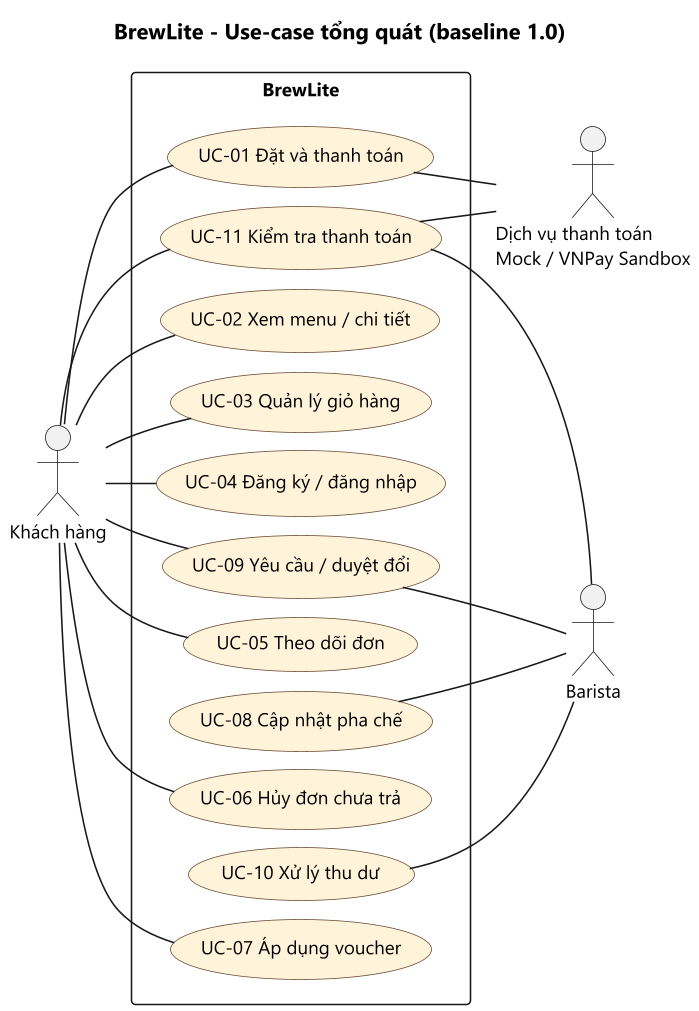
\includegraphics[width=.95\linewidth,height=.68\textheight,keepaspectratio]{../docs/diagrams/usecase-system.png}
\caption{Use-case tổng quát, có nguồn PlantUML và bản SVG trong docs/diagrams}
\end{figure}
\begin{figure}[htbp]\centering
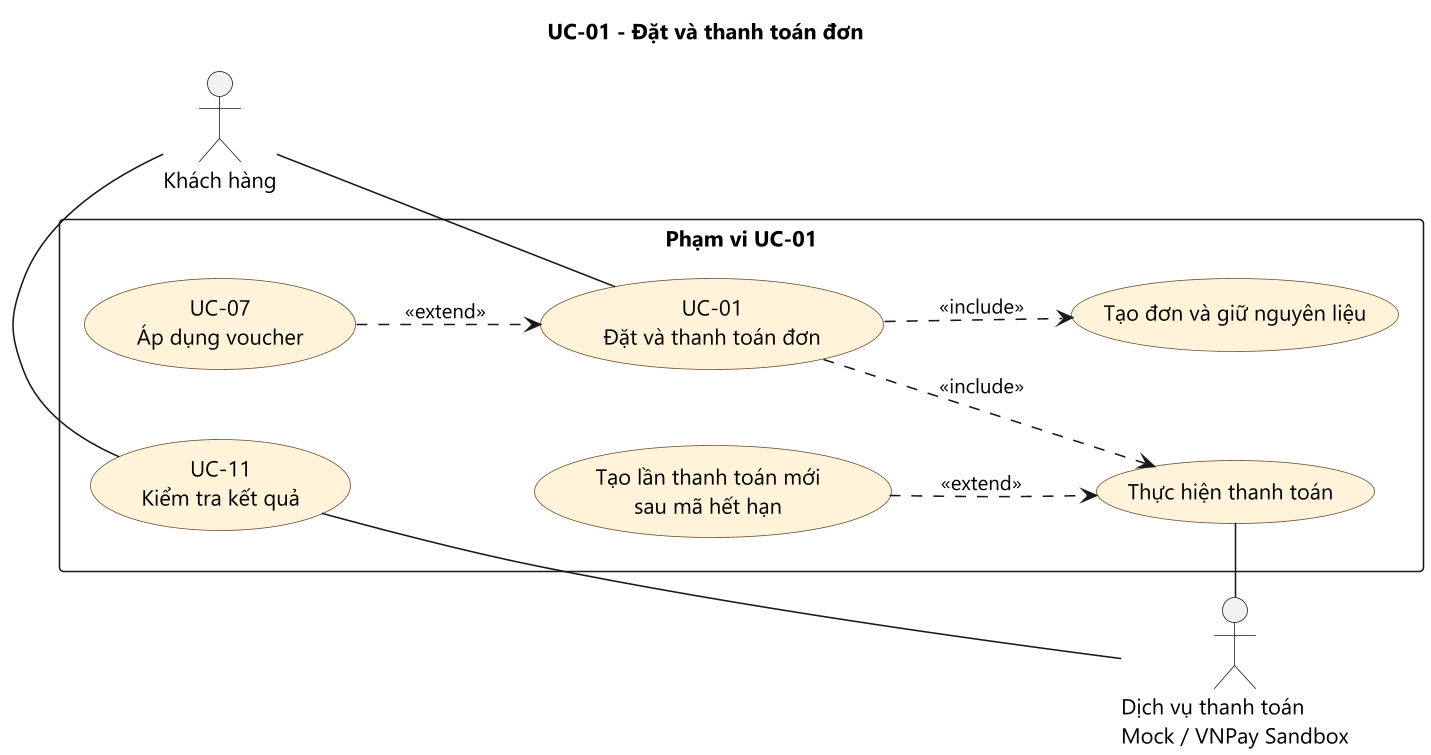
\includegraphics[width=\linewidth,height=.48\textheight,keepaspectratio]{../docs/diagrams/usecase-checkout.png}
\caption{Phạm vi UC-01: đặt và thanh toán đơn}
\end{figure}

\subsection{Yêu cầu nghiệp vụ đặt hàng, giữ kho và hoàn kho}
\label{sec:inventory-requirements}
Luồng đặt hàng được tổ chức thành ba thời điểm riêng biệt: khách chọn món, backend tạo đơn và hệ thống xác minh thanh toán. Việc thêm món vào giỏ chỉ lưu lựa chọn ở trình duyệt. Nguyên liệu được giữ khi backend chấp nhận tạo Order ở trạng thái PENDING; thanh toán thành công xác nhận quyền phục vụ đơn đã giữ, không trừ nguyên liệu thêm một lần nữa.

\begin{longtable}{|p{.12\linewidth}|p{.79\linewidth}|}
\hline\textbf{Mã quy tắc} & \textbf{Nội dung và tiêu chí chấp nhận}\\\hline\endhead
INV-01 & Chỉ khách đã xác thực được tạo đơn. Backend kiểm tra sản phẩm, size, topping, số lượng và voucher; tự tính giá. Yêu cầu không hợp lệ không tạo đơn hoặc làm thay đổi kho.\\\hline
INV-02 & Khi tạo đơn, cộng gộp nhu cầu nguyên liệu của tất cả món và topping. Một nguyên liệu dùng chung chỉ có một tổng lượng cần giữ; vật tư không tăng theo size được tính riêng.\\\hline
INV-03 & Kiểm kho, trừ nguyên liệu, lưu Order/OrderItem, snapshot và kết quả idempotency thuộc cùng transaction. Một bước thất bại phải hoàn tác toàn bộ các thay đổi trong transaction.\\\hline
INV-04 & Nhiều khách tranh phần nguyên liệu cuối: tổng lượng giữ thành công không vượt tồn thực tế. Cùng khách, cùng key và cùng nội dung phải trả lại đơn cũ, không trừ kho lần hai.\\\hline
INV-05 & Khách chỉ tự hủy đơn PENDING hoặc PAYMENT\_FAILED chưa sử dụng credit chuyển từ đơn cũ; phải sở hữu đơn. Giao dịch còn cần xác minh được kiểm tra trước khi cho hủy. Đơn PAID không đi qua API hủy thông thường.\\\hline
INV-06 & Hủy hợp lệ hoàn theo lượng đã lưu tại thời điểm đặt, không theo Recipe hiện tại. Hủy đồng thời hoặc gọi hoàn lại không được cộng kho hai lần; thiếu bằng chứng snapshot phải chuyển quầy kiểm tra.\\\hline
INV-07 & Đơn chưa thanh toán có thời hạn giữ món mặc định 30 phút. Hết hạn, backend chặn thanh toán mới và tác vụ nền đóng đơn đủ điều kiện, hoàn snapshot; giao diện thông báo khách đặt lại.\\\hline
INV-08 & Thời hạn QR không vượt thời hạn giữ món. QR hết hạn trước deadline của đơn được cấp lại; việc cấp QR không tự gia hạn giữ nguyên liệu. Tiền về muộn được ghi nhận vào quy trình xử lý khoản thu không áp dụng.\\\hline
INV-09 & Đơn đã có Payment, bằng chứng đã nhận tiền hoặc credit chuyển từ đơn cũ được bảo toàn để quầy xử lý; không tự đóng như đơn bỏ thanh toán thông thường. Khi duyệt đổi món, hoàn lượng cũ và giữ lượng mới phải cùng thành công hoặc cùng rollback.\\\hline
\caption{Quy tắc và tiêu chí chấp nhận của luồng quản lý nguyên liệu}
\end{longtable}

Ví dụ, khách chọn hai ly M có topping trong giỏ chưa làm kho giảm. Sau khi gửi đặt hàng thành công, lượng nguyên liệu đã giữ được ghi cùng mã đơn. Nếu khách chưa thanh toán và hủy hợp lệ, lượng này được cộng lại. Nếu khách trả tiền thành công, đơn chuyển PAID và quầy tiếp nhận; kho không bị trừ lần nữa khi chuyển trạng thái.


\section{Thiết kế hệ thống}
\subsection{Kiến trúc tổng thể}
Frontend Next.js gọi REST API của backend NestJS bằng JSON. Backend dùng Prisma để làm việc với PostgreSQL và tích hợp cổng thanh toán giả lập (mock payment gateway) dưới dạng một service riêng trong backend.

\begin{figure}[h!]
\centering
\begin{tikzpicture}[box/.style={draw,rounded corners,minimum width=3cm,minimum height=1.2cm,align=center,font=\small},>=stealth]
	\node[box] (fe) at (0,0) {Next.js\\(giao diện)};
	\node[box] (be) at (5,0) {NestJS\\(REST API)};
	\node[box] (db) at (10,0) {PostgreSQL};
	\node[box] (pay) at (5,-2.4) {Cổng thanh toán\\giả lập (mock)};
	\draw[->] (fe) -- node[above,font=\scriptsize] {REST/JSON} (be);
	\draw[->] (be) -- node[above,font=\scriptsize] {Prisma ORM} (db);
	\draw[->] (be) -- node[right,font=\scriptsize] {thanh toán} (pay);
\end{tikzpicture}
\caption{Kiến trúc tổng thể của hệ thống}
\end{figure}

\subsection{Mô hình dữ liệu}
\begin{table}[h!]
\centering
\footnotesize
\begin{tabularx}{\textwidth}{|l|X|}
\hline
\textbf{Thực thể} & \textbf{Thuộc tính} \\ \hline
Product & id, name, price, imageUrl; tồn kho được suy ra từ nguyên liệu và công thức \\ \hline
User & id, email (duy nhất), passwordHash, loyaltyPoints \\ \hline
Voucher & id, code (duy nhất), discountPercent, expiresAt, active \\ \hline
Order & id, userId, status, total, discount, voucherId, createdAt \\ \hline
OrderItem & id, orderId, productId, size, toppings, qty, lineTotal \\ \hline
Payment & id, orderId, idempotencyKey (duy nhất), amount, method, createdAt \\ \hline
\end{tabularx}
\caption{Các thực thể của hệ thống}
\end{table}

Quan hệ: một User có nhiều Order; một Order có nhiều OrderItem và Payment; OrderItem tham chiếu Product. Ingredient và Recipe biểu diễn nguyên liệu và định lượng theo món. OrderInventoryReservation lưu từng dòng nguyên liệu đã giữ của từng đơn, tách biệt công thức hiện tại. OrderCreateRequest lưu khóa chống tạo đơn trùng; VnpayAttempt lưu từng lần thanh toán VNPay; OrderExchange lưu yêu cầu đổi món; PaymentRefundCase lưu hồ sơ xử lý khoản thu dư. LoyaltyTransaction là sổ giao dịch điểm thưởng. Phần giải thích bên dưới trình bày mục đích và ví dụ của các bảng bổ sung.

\subsubsection{Các thực thể phục vụ quản lý nguyên liệu}
\label{sec:inventory-data}
Product biểu diễn món bán cho khách; Ingredient biểu diễn tài nguyên thật trong kho. Một nguyên liệu có thể được dùng cho nhiều món, vì vậy không thể coi số phần của mỗi Product là một kho độc lập. Ví dụ cà phê sữa và Americano cùng dùng cà phê rang xay: bán một món sẽ làm giảm khả năng bán món còn lại.

\begin{longtable}{|p{.33\linewidth}|p{.58\linewidth}|}
\hline\textbf{Thành phần} & \textbf{Vai trò và lý do thiết kế}\\\hline\endhead
Ingredient & Lưu id, tên, đơn vị và stock bằng số nguyên theo đơn vị nhỏ nhất (g, ml, cái). Ràng buộc stock không âm bảo vệ dữ liệu ở database.\\\hline
Recipe & Bảng liên kết Product--Ingredient. quantity là định lượng một ly size S; cặp productId/ingredientId duy nhất ngăn khai báo trùng thành phần của cùng công thức. quantity phải dương.\\\hline
Recipe.scalesWithSize & Quyết định lượng có tăng theo size hay không. Cà phê, sữa có thể tăng; ly, nắp thường giữ một cái cho mỗi ly. Không suy ra điều này từ giá bán.\\\hline
ToppingRecipe & Lưu toppingCode, ingredientId và quantity cho một phần topping. Một topping có thể dùng nhiều nguyên liệu; một nguyên liệu có thể vừa thuộc công thức món vừa thuộc topping. Bảng riêng tránh lặp toàn bộ topping cho mỗi món.\\\hline
Order và OrderItem & Order lưu trạng thái và giá trị đơn; OrderItem lưu món, size, topping và số lượng đã chọn. Những lựa chọn này là đầu vào để tính lượng cần giữ.\\\hline
OrderInventoryReservation & Một dòng cho mỗi cặp orderId/ingredientId: quantity lưu chính tổng lượng đã trừ, releasedAt cho biết đã hoàn hay chưa. Đây là snapshot tài nguyên của đơn, không phải công thức sản phẩm thứ hai.\\\hline
Order.reservationExpiresAt & Deadline giữ món được lưu bền vững, dùng chung cho worker, API thanh toán và giao diện. Không phụ thuộc thời điểm khách tải lại trang.\\\hline
Order.reservationExpiredAt & Ghi thời điểm hệ thống đóng do hết hạn; phân biệt với khách chủ động hủy hoặc đơn cũ được thay thế khi đổi món dù đều dùng trạng thái CANCELLED.\\\hline
OrderCreateRequest & Lưu khách, idempotency key, dấu vân tay nội dung và Order kết quả. Ngăn retry tạo thêm đơn và giữ thêm nguyên liệu.\\\hline
\caption{Dữ liệu và trách nhiệm của các bảng trong luồng giữ/hoàn kho}
\end{longtable}

Một Order có nhiều snapshot nguyên liệu; một Ingredient xuất hiện trong snapshot của nhiều Order. Unique(orderId, ingredientId) thể hiện việc cộng gộp trước khi lưu. Quan hệ snapshot tham chiếu nguyên liệu dùng quy tắc Restrict khi xóa, giữ bằng chứng lịch sử ngay cả khi công thức Recipe đã được thay đổi hoặc xóa. OrderItem lưu lựa chọn mua, còn snapshot lưu tài nguyên đã tiêu hao để giữ chỗ: hai loại dữ liệu phục vụ hai mục đích khác nhau.

\begin{sidewaysfigure}\centering
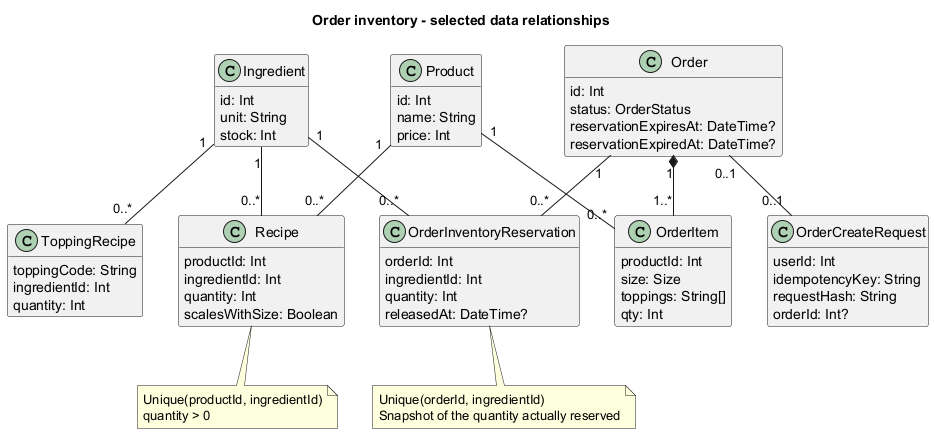
\includegraphics[width=.95\textheight,height=.85\textwidth,keepaspectratio]{assets/inventory/inventory-relations.png}
\caption{Quan hệ dữ liệu của đặt hàng, công thức và snapshot nguyên liệu}
\label{fig:inventory-relations}
\end{sidewaysfigure}


\begin{lstlisting}[style=brew]
model Payment {
  id             Int           @id @default(autoincrement())
  orderId        Int
  idempotencyKey String        @unique
  amount         Int
  method         PaymentMethod
  createdAt      DateTime      @default(now())
}
\end{lstlisting}

\subsection{Thiết kế API}
\begin{table}[h!]
\centering
\footnotesize
\begin{tabularx}{\textwidth}{|l|l|X|c|}
\hline
\textbf{Phương thức} & \textbf{Đường dẫn} & \textbf{Chức năng} & \textbf{Đăng nhập} \\ \hline
GET & \texttt{/products} & Danh sách sản phẩm & Không \\ \hline
GET & \texttt{/products/:id} & Chi tiết sản phẩm, kèm bảng size và topping & Không \\ \hline
POST & \texttt{/auth/register} & Đăng ký, trả JWT & Không \\ \hline
POST & \texttt{/auth/login} & Đăng nhập, trả JWT & Không \\ \hline
GET & \texttt{/auth/me} & Thông tin người dùng hiện tại & Có \\ \hline
POST & \texttt{/promotions/validate} & Kiểm tra mã giảm giá & Không \\ \hline
POST & \texttt{/orders} & Tạo đơn PENDING (kèm \texttt{voucherCode} tùy chọn) & Có \\ \hline
GET & \texttt{/orders/me} & Lịch sử đơn của người dùng & Có \\ \hline
GET & \texttt{/orders/:id} & Chi tiết một đơn & Có \\ \hline
POST & \texttt{/orders/:id/cancel} & Hủy đơn & Có \\ \hline
POST & \texttt{/payments} & Thanh toán, bắt buộc header \texttt{Idempotency-Key} & Có \\ \hline
\end{tabularx}
\caption{Các API của backend}
\end{table}

\subsubsection{Thiết kế xác thực và phân quyền}
\label{sec:auth-design}
Hệ thống tách ba câu hỏi: người gọi là ai (JWT), có vai trò nào (Role), và có quyền trên đối tượng cụ thể không (chủ đơn). User lưu email duy nhất, passwordHash, role và điểm; role mặc định CUSTOMER. API đăng ký công khai không nhận quyền BARISTA từ dữ liệu khách gửi. Tài khoản quầy được cấp qua quy trình quản trị dữ liệu.

\begin{table}[htbp]\centering\small
\begin{tabularx}{\linewidth}{|p{.31\linewidth}|X|}\hline
\textbf{Nhóm thao tác} & \textbf{Điều kiện backend}\\\hline
Menu, chi tiết; đăng ký/đăng nhập & Được truy cập không cần JWT; input đăng ký/đăng nhập vẫn qua DTO validation.\\\hline
Thông tin tài khoản hiện tại & JWT hợp lệ; danh tính lấy từ token đã xác minh và User trong database.\\\hline
Xem/tạo/hủy/thanh toán đơn cá nhân & JWT hợp lệ và điều kiện nghiệp vụ; khi thao tác trên đơn có sẵn phải kiểm userId là chủ đơn.\\\hline
Hàng đợi, cập nhật trạng thái và quyết định của quầy & JWT hợp lệ, role BARISTA và luật trạng thái/version/transaction tương ứng.\\\hline
Khách xem/rút yêu cầu đổi & JWT và chủ Order nguồn; không có quyền tự duyệt hoặc tự xác nhận hoàn khoản thu dư.\\\hline
IPN/Return từ VNPay & Dữ liệu giao thức được kiểm chữ ký và tham chiếu, không dùng JWT của khách làm chứng thực callback cổng.\\\hline
\end{tabularx}\caption{Điều kiện truy cập theo danh tính, vai trò và chủ thể dữ liệu}
\end{table}

Thiếu token, token không hợp lệ/hết hạn hoặc người dùng không còn tồn tại bị từ chối xác thực (401). Tài khoản đã xác thực nhưng không có vai trò staff bị từ chối quyền (403). Với API đọc/hủy đơn cá nhân, đơn không thuộc người gọi được trả như không tìm thấy (404). Các mã lỗi có phạm vi khác nhau; việc ẩn nút quầy trên frontend không thay thế kiểm tra backend.

\begin{figure}[htbp]\centering
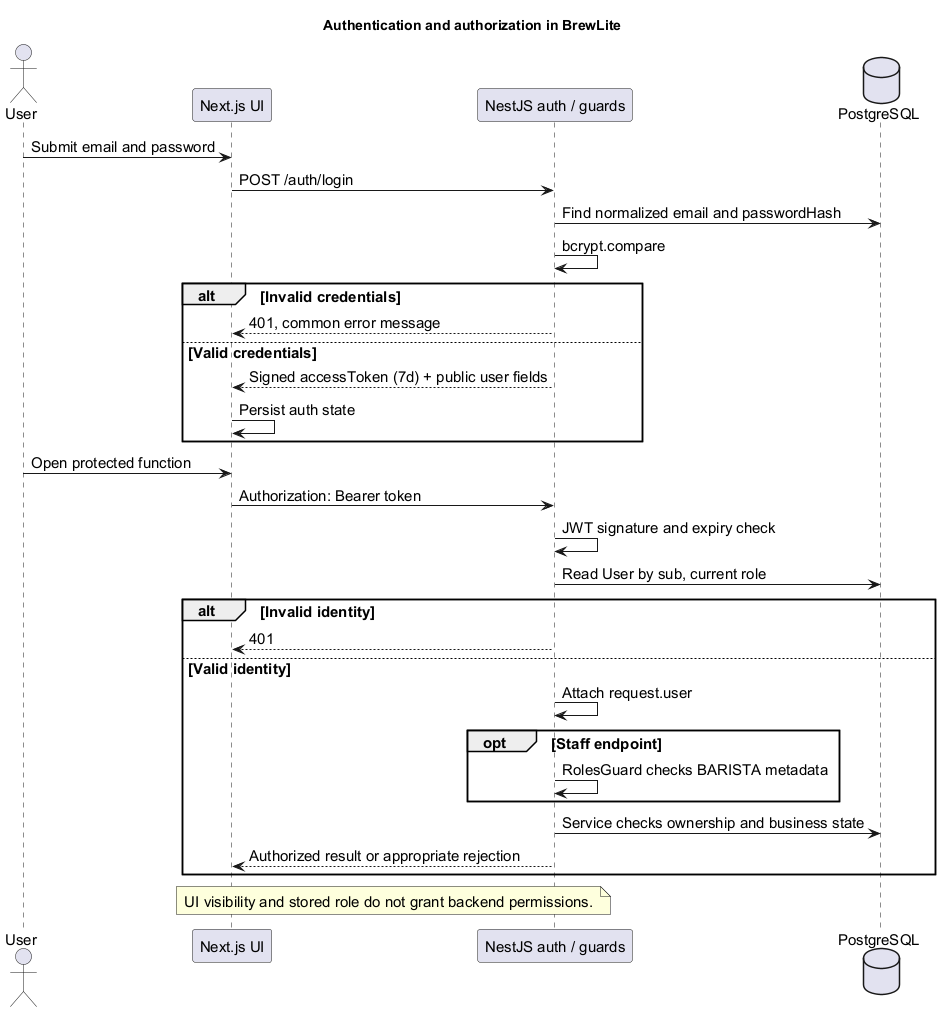
\includegraphics[width=\linewidth,height=.54\textheight,keepaspectratio]{assets/auth/auth-sequence.png}
\caption{Đăng nhập cấp token và chuỗi kiểm danh tính, vai trò, chủ đơn ở backend}
\end{figure}


\subsection{Máy trạng thái đơn hàng (Order State Machine)}
Mỗi đơn hàng tại một thời điểm chỉ ở đúng một trạng thái và chỉ được đổi theo các chuyển tiếp hợp lệ. Mọi chuyển tiếp không có trong sơ đồ bị hàm \texttt{assertTransition} chặn lại bằng lỗi. COMPLETED và CANCELLED là trạng thái kết thúc.

\begin{figure}[h!]
\centering
\resizebox{\linewidth}{!}{%
\begin{tikzpicture}[st/.style={draw,rounded corners,minimum width=2.5cm,minimum height=0.9cm,font=\small\ttfamily,align=center},>=stealth]
	\node[st] (pending) at (0,0) {PENDING};
	\node[st] (paid) at (3.9,0) {PAID};
	\node[st] (prep) at (7.8,0) {PREPARING};
	\node[st] (ready) at (11.7,0) {READY};
	\node[st,double] (done) at (15.6,0) {COMPLETED};
	\node[st,minimum width=3.6cm] (failed) at (3.9,-2.6) {PAYMENT\_FAILED};
	\node[st,double] (canc) at (0,-5.2) {CANCELLED};
	\draw[->] (pending) -- (paid);
	\draw[->] (paid) -- (prep);
	\draw[->] (prep) -- (ready);
	\draw[->] (ready) -- (done);
	\draw[->] (pending) to[bend left=15] (failed);
	\draw[->] (failed) to[bend left=15] (pending);
	\draw[->] (failed) -- (paid);
	\draw[->] (pending) -- (canc);
	\draw[->] (failed) -- (canc);
\draw[->] (paid.east) -- (6.1,0) -- (6.1,-5.2) -- node[above,font=\scriptsize] {Duyệt đổi món} (canc.east);
\end{tikzpicture}}
\caption{Sơ đồ máy trạng thái của đơn hàng}
\end{figure}

\begin{table}[h!]
\centering
\footnotesize
\begin{tabularx}{\textwidth}{|p{0.22\linewidth}|p{0.28\linewidth}|X|}
\hline
\textbf{Từ} & \textbf{Sang} & \textbf{Sự kiện} \\ \hline
PENDING & PAID & Thanh toán thành công \\ \hline
PENDING & PAYMENT\_FAILED & Thanh toán lỗi \\ \hline
PENDING & CANCELLED & Khách hủy đơn \\ \hline
PAYMENT\_FAILED & PENDING hoặc PAID & Thử thanh toán lại \\ \hline
PAYMENT\_FAILED & CANCELLED & Khách hủy đơn \\ \hline
PAID & CANCELLED & Chỉ khi yêu cầu đổi món được duyệt, chuyển giá trị sang đơn mới \\ \hline
PAID & PREPARING & Barista nhận pha chế \\ \hline
PREPARING & READY & Pha xong \\ \hline
READY & COMPLETED & Giao cho khách \\ \hline
\end{tabularx}
\caption{Các chuyển trạng thái hợp lệ}
\end{table}

Khách không được tự hủy đơn PAID. Chuyển PAID sang CANCELLED chỉ được thực hiện trong nghiệp vụ đổi món đã được barista duyệt, đồng thời chuyển giá trị đã trả sang đơn thay thế. Máy trạng thái chỉ kiểm tra chuyển tiếp; service phải kiểm tra quyền, điều kiện và giao dịch nguyên tử. Giao diện barista xử lý PREPARING, READY và COMPLETED. Khi đã pha chế, không áp dụng luồng đổi món này.

\subsubsection{Vận hành quầy và đồng bộ trạng thái}
\label{sec:staff-design}
Barista xử lý theo chuỗi PAID $\rightarrow$ PREPARING $\rightarrow$ READY $\rightarrow$ COMPLETED trên bảng bốn cột: chờ duyệt, đang pha, sẵn sàng và hoàn tất. Đơn PENDING/PAYMENT\_FAILED/CANCELLED không vào hàng đợi pha chế. Thao tác quầy chỉ đổi trạng thái phục vụ, không tạo Payment, giữ nguyên liệu hoặc cộng điểm lần nữa. Quyền BARISTA áp dụng ở backend như mục~\ref{sec:auth-design}.

findForStaff lấy mọi đơn đang xử lý theo createdAt/id tăng dần và tối đa 20 đơn hoàn tất gần nhất. Hai nhóm được đọc trong transaction RepeatableRead để tránh một đơn vừa chuyển COMPLETED bị mất hoặc lặp do đọc ở hai thời điểm khác nhau. Giới hạn 20 chỉ áp dụng nhóm hoàn tất, không cắt mất đơn đang chờ làm.

Đơn có yêu cầu đổi REQUESTED phải được duyệt/từ chối/rút trước khi bắt đầu pha. Khi quầy cập nhật thành công, backend commit rồi phát sự kiện orders.changed. Sự kiện chỉ báo có thay đổi, không mang thông tin đơn/tài khoản; client gọi lại API có xác thực và quyền đọc tương ứng. WebSocket là tín hiệu đồng bộ, còn database/API là nguồn trạng thái thật.

\begin{figure}[htbp]\centering
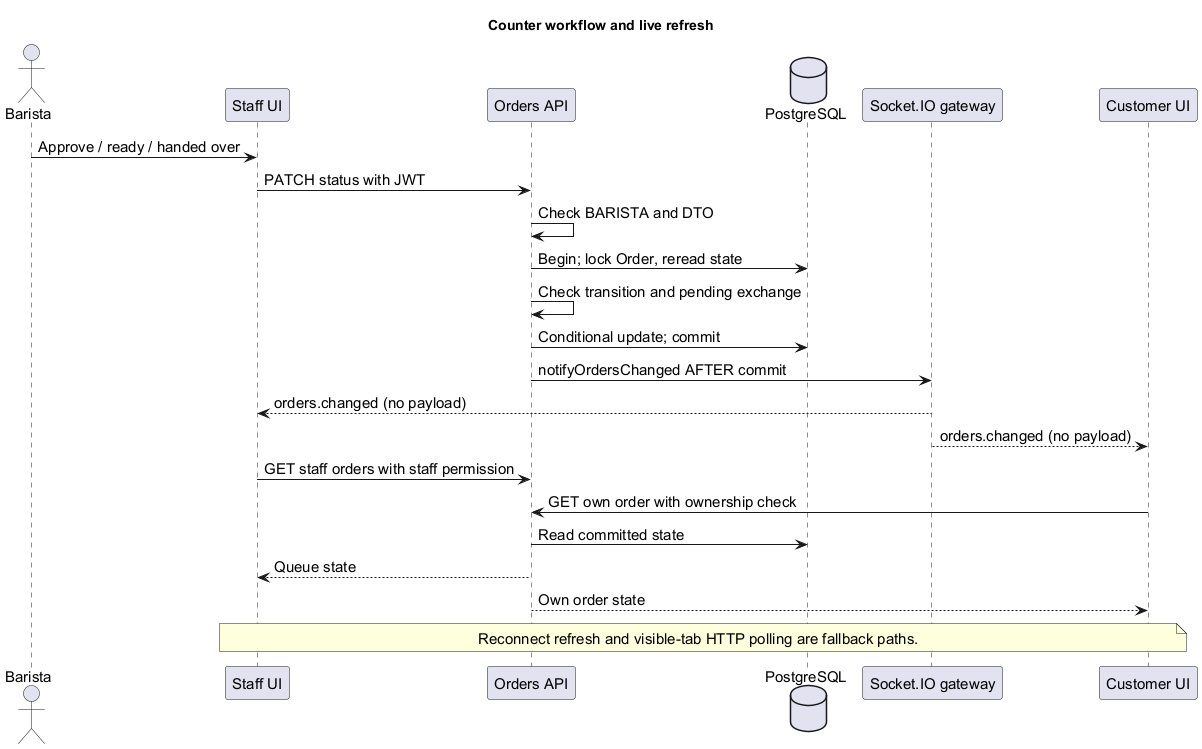
\includegraphics[width=\linewidth,height=.49\textheight,keepaspectratio]{assets/staff/staff-realtime.png}
\caption{Cập nhật trạng thái tại quầy, commit rồi thông báo để mỗi client đọc lại API được phép}
\end{figure}


\subsection{Quy tắc tính giá, giảm giá và điểm thưởng}
\begin{itemize}
	\item \textbf{Giá một ly} = giá menu (giá size S) + phụ thu size + phụ thu topping. Phụ thu size: S cộng 0đ, M cộng 5.000đ, L cộng 10.000đ. Mỗi topping (Trân châu, Kem) cộng 5.000đ. Ví dụ: Cappuccino 45.000đ, size L, thêm Trân châu là 45.000 + 10.000 + 5.000 = 60.000đ.
	\item \textbf{Mã giảm giá:} giảm theo phần trăm, làm tròn xuống đến đồng, không giảm quá tổng tiền; mã có hạn dùng và có thể bị tắt. Mã mẫu BREW10 giảm 10\%.
	\item \textbf{Điểm thưởng:} khách được cộng 1 điểm cho mỗi 10.000đ đã thanh toán (tính trên số tiền sau giảm), cộng khi đơn chuyển sang PAID.
\end{itemize}
Các mức phụ thu, mức giảm và tỷ lệ điểm là chính sách cấu hình của cửa hàng.
\subsubsection{Mã giảm giá và giá trị đơn đã chốt}
Voucher lưu code duy nhất, discountPercent, expiresAt và active; Order liên kết voucherId đồng thời lưu discount và total. Liên kết chỉ ra mã đã áp dụng, còn hai số tiền trên Order giữ giá trị giao dịch đã tính, không tính lại theo cấu hình voucher khi khách thanh toán sau đó.

Backend chuẩn hóa mã bằng trim/uppercase, kiểm tồn tại, active và expiresAt. Endpoint validate phục vụ xem trước; lúc tạo đơn vẫn kiểm lại trong transaction trước khi reserve nguyên liệu. Giá frontend hiển thị không thay thế phép tính backend.

\[
 discount=\min\left(subtotal,\left\lfloor subtotal\times\frac{p}{100}\right\rfloor\right),
 \qquad total=subtotal-discount.
\]
Trong hàm tính, $p$ được giới hạn trong khoảng 0--100. Ví dụ 120.000đ áp BREW10 giảm 12.000đ, còn 108.000đ. Mã không hợp lệ làm yêu cầu tạo đơn bị từ chối trước khi thay đổi kho.

\subsubsection{Số dư điểm và sổ giao dịch điểm}
User.loyaltyPoints là số dư hiện tại để đọc nhanh. LoyaltyTransaction lưu userId, orderId, loại, points, balanceAfter và thời gian để giải thích mỗi lần biến động. Unique(orderId, type) ngăn ghi hai dòng EARN cho cùng Order; balanceAfter ghi số dư sau lần cộng đó.

Chính sách hiện tại là $points=\max(0,\lfloor amount/10.000\rfloor)$ theo khoản thanh toán mới được áp dụng. Đơn sau giảm 108.000đ được 10 điểm; dưới 10.000đ không tạo dòng EARN. Khi đổi món, tiền chuyển từ đơn cũ không cộng lại điểm; phần thu thêm được tính tại đơn thay thế. Điểm được làm tròn theo mỗi lần áp dụng, không gom phần tiền lẻ giữa các đơn.


\subsection{VNPay Sandbox và xác minh kết quả}
\label{sec:vnpay-design}
Tích hợp VNPay sử dụng ba thành phần: frontend hiển thị QR/liên kết và trạng thái; NestJS tạo yêu cầu, kiểm chứng kết quả và ghi sổ; VNPay Sandbox xử lý phiên thanh toán thử. QR chứa URL mở trang VNPay, không phải QR chuyển khoản trực tiếp của ứng dụng ngân hàng. Chữ ký và khóa merchant chỉ được xử lý ở backend. Cách phân biệt Return/IPN và quy tắc tham số được đối chiếu với tài liệu VNPay~\cite{VNPAYPAY,VNPAYFAQ}.

\subsubsection{Phân biệt đơn hàng, lần thanh toán và khoản áp dụng}
\begin{table}[htbp]\centering\small
\begin{tabularx}{\linewidth}{|p{.30\linewidth}|X|}\hline
\textbf{Thực thể} & \textbf{Trách nhiệm}\\\hline
Order & Nghĩa vụ phục vụ và tiền còn cần thu: total trừ creditApplied. Một đơn có thể thử thanh toán nhiều lần.\\\hline
VnpayAttempt & Mỗi lần giao dịch có txnRef duy nhất, số tiền, URL, hạn, mã giao dịch nhà cung cấp và trạng thái riêng; giữ lịch sử cả lần thất bại/chưa rõ.\\\hline
PaymentStartRequest & Ánh xạ cặp khách/key tới attempt để gửi lại yêu cầu không tạo thêm lần thanh toán. Key mới vẫn có thể tái dùng mã đang hiệu lực.\\\hline
Payment & Khoản đã xác minh và áp dụng vào Order; không tạo cho mọi attempt hoặc tiền thu nhưng không thể phục vụ. Liên kết attempt duy nhất chống ghi nhận lại cùng lần.\\\hline
PaymentAudit & Nhật ký tạo mã, tra cứu, nhận kết quả và thao tác hỗ trợ; phục vụ truy vết theo attempt, actor và thời gian.\\\hline
PaymentRefundCase & Hồ sơ khoản đã thu nhưng không áp dụng được (thu trùng, đơn không còn hiệu lực); một hồ sơ theo attempt, quầy xử lý bằng chứng từ.\\\hline
\end{tabularx}\caption{Phân tách dữ liệu thanh toán để bảo toàn lịch sử và tránh ghi nhận trùng}
\end{table}

Ví dụ đơn 75.000đ đã chuyển credit 45.000đ chỉ cần thu thêm 30.000đ. Backend ký đúng phần còn thu; frontend không tự quyết định số tiền. Nếu lần A hết hạn rồi cấp B và cả hai cùng thu thành công, chỉ một khoản được áp dụng cho đơn; khoản còn lại có attempt và hồ sơ xử lý riêng, không tạo hai đơn pha chế.

\subsubsection{Luồng và các nhánh kết quả}
Backend kiểm chủ đơn, PENDING/PAYMENT\_FAILED, deadline và snapshot chưa hoàn trước khi cấp mã. Lần mới có txnRef riêng; amount lưu VND nguyên, trường vnp\_Amount gửi sang cổng nhân 100 theo giao thức. Các trường được chuẩn hóa và ký HMAC-SHA512. Hạn QR bị giới hạn bởi deadline giữ món đã trình bày ở mục~\ref{sec:inventory-demand}.

Return xác minh chữ ký, merchant, tham chiếu và số tiền rồi trả HTTP 303 về trang Order; không chuyển PAID. IPN là thông báo server-to-server; QueryDr là truy vấn backend chủ động khi cần kiểm tra. Cả hai kết quả đã xác minh được quy về apply để cùng kiểm soát ghi nhận. Mất Return hoặc khách đóng tab không xóa kết quả đã commit.

\begin{table}[htbp]\centering\small
\begin{tabularx}{\linewidth}{|p{.32\linewidth}|X|}\hline
\textbf{Tình huống} & \textbf{Xử lý trong hệ thống}\\\hline
Thành công, đơn còn đủ điều kiện & Ghi Payment, PAID và điểm trên tiền mới trong cùng transaction; không giữ kho thêm.\\\hline
Thất bại đã xác minh & Ghi FAILED/EXPIRED theo kết quả; đơn còn hạn có thể bắt đầu lần khác.\\\hline
Timeout hoặc kết quả chưa rõ & Giữ lịch sử PENDING/REVIEW, không tự suy ra thất bại. QueryDr chạy ngoài transaction; việc cấp mã mới tuân điều kiện hạn mã/đơn và bằng chứng tiền đã thu.\\\hline
QR hết hạn, đơn còn hạn & Thử tra cứu rồi có thể cấp lần mới dù tra cứu chưa kết luận; giữ attempt cũ để nhận kết quả muộn.\\\hline
IPN lặp hoặc đến ngược thứ tự & Kết quả đã ghi không được ghi lại/cộng điểm lại; thông báo thất bại đến sau không hạ PAID.\\\hline
Thu trùng hoặc tiền về sau khi đơn không còn hiệu lực & Ghi REVIEW và hồ sơ khoản thu không áp dụng; không tự mở lại đơn/pha chế.\\\hline
\end{tabularx}\caption{Quy tắc xử lý kết quả VNPay và thanh toán lại}
\end{table}

\begin{figure}[htbp]\centering
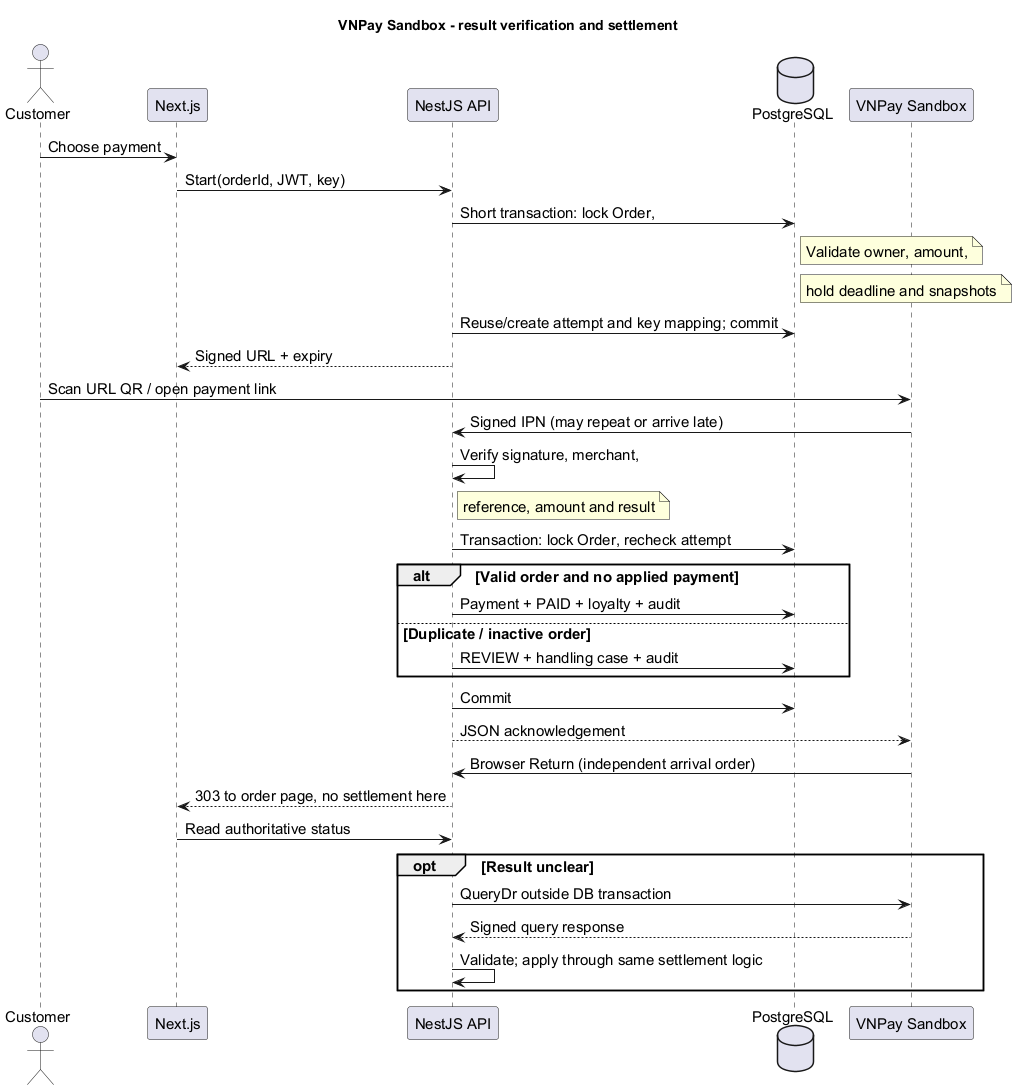
\includegraphics[width=\linewidth,height=.62\textheight,keepaspectratio]{assets/vnpay/vnpay-sequence.png}
\caption{Luồng VNPay: Return điều hướng, IPN/QueryDr xác minh và ghi nhận tại backend}
\end{figure}


\subsection{Giữ kho và hoàn theo snapshot}
\subsubsection{Định lượng theo size và topping}
\label{sec:inventory-demand}
Với mỗi dòng món, backend lấy định lượng size S từ Recipe. Chính sách định lượng đang dùng có hệ số S = 100\%, M = 125\%, L = 150\%; đây là cấu hình nghiệp vụ, độc lập phụ thu giá size. Thành phần có scalesWithSize=true được nhân hệ số rồi làm tròn lên theo từng ly. Thành phần có scalesWithSize=false giữ nguyên lượng. Sau đó cộng định lượng topping của một ly và nhân số ly; cuối cùng gộp tất cả dòng theo ingredientId.

Gọi $q_{ig}$ là lượng cơ bản nguyên liệu $g$ của món $i$, $r_s$ là hệ số size, $n_i$ là số ly và $t_{ig}$ là tổng lượng nguyên liệu $g$ từ topping của một ly. Khi thành phần tăng theo size:
\[
 D_g=\sum_i n_i\left(\left\lceil q_{ig}r_s\right\rceil+t_{ig}\right).
\]
Nếu không tăng theo size, thay $\lceil q_{ig}r_s\rceil$ bằng $q_{ig}$. Việc làm tròn trước khi nhân số ly bảo đảm mỗi ly đều có đủ lượng theo định mức nguyên.

\begin{table}[htbp]\centering\small
\begin{tabularx}{\linewidth}{|X|c|c|}\hline
\textbf{Thành phần} & \textbf{Một ly M} & \textbf{Hai ly M}\\\hline
Cà phê cơ bản 18g, tăng theo size & $\lceil18\times1{,}25\rceil=23$g & 46g\\\hline
Topping dùng thêm 5g cùng nguyên liệu & 5g & 10g\\\hline
Ly nhựa, không tăng theo size & 1 cái & 2 cái\\\hline
Tổng cà phê phải giữ & 28g & 56g\\\hline
\end{tabularx}\caption{Ví dụ minh họa cộng gộp định lượng, không phải công thức mặc định của topping Kem}
\end{table}

Hàm ingredientDemand dùng chung cho kiểm kho khi đặt và tính availability trên menu. Với lựa chọn một ly, số ly có thể bán bằng giá trị nhỏ nhất của $\lfloor stock_g/D_g\rfloor$ trên các nguyên liệu cần dùng. Do topping có thể dùng chung nguyên liệu với món, phải gộp demand trước khi chia; tính riêng hai phần rồi lấy min có thể báo còn hàng sai. Availability ở giao diện là ảnh chụp tham khảo; backend luôn kiểm lại tại transaction tạo đơn hoặc duyệt đổi món.

\subsubsection{Snapshot: vì sao không hoàn bằng công thức hiện tại?}
Recipe mô tả định mức bán hiện hành, trong khi snapshot là bằng chứng lượng đã giữ của một đơn cụ thể. Ví dụ khi đặt, một ly giữ 20g cà phê. Sau đó quầy sửa Recipe thành 25g. Nếu hủy bằng công thức mới, hệ thống cộng 25g dù trước đó chỉ trừ 20g, tạo ra 5g không có thật. Snapshot giữ quantity=20 nên hoàn đúng 20g. Thay topping, hệ số size hay chuyển công thức sang nguyên liệu khác cũng không thay đổi snapshot đã lưu.

Snapshot được tạo từ chính Map demand đã dùng để trừ kho, trong cùng transaction với Order. Không đọc lại Recipe sau bước trừ để dựng snapshot, vì lần đọc khác có thể không đại diện lượng vừa giữ. releasedAt là dấu hoàn; quantity vẫn giữ nguyên để tra cứu lịch sử. Một đơn có nhiều dòng món cùng dùng cà phê sẽ có một snapshot cà phê tổng, vì khi hủy toàn đơn chỉ cần trả đúng tổng lượng đã giữ.

\subsubsection{Hủy chủ động và hết thời gian giữ món}
Hủy chủ động kiểm tra chủ đơn, trạng thái và điều kiện thanh toán. Khách chỉ tự hủy PENDING/PAYMENT\_FAILED không có credit; backend khóa Order, kiểm tra các attempt cần xác minh, cập nhật trạng thái có điều kiện rồi release snapshot trong cùng transaction. Nếu bước hoàn bị lỗi thì trạng thái hủy cũng rollback. PAID và các trạng thái pha chế không dùng API hủy thông thường; đổi món đã trả tiền đi qua yêu cầu và quyết định của barista.

Với đơn bỏ thanh toán, reservationExpiresAt mặc định cách lúc tạo 30 phút. ReservationExpiryService quét khi khởi động và mỗi 30 giây, tối đa 100 đơn/lượt. Chỉ đóng đơn chưa trả tiền, chưa có bằng chứng đã thu và chưa sử dụng credit. Khi đủ điều kiện, worker hoàn snapshot và ghi CANCELLED cùng reservationExpiredAt; thông báo được phát sau commit. Giao diện hiển thị ``Đã hết thời gian đặt món, vui lòng đặt lại.'' và đưa khách về menu để tạo yêu cầu mua mới.

Deadline của đơn và deadline QR là hai giá trị khác nhau. Ví dụ đơn giữ món từ 10:00 đến 10:30; QR đầu hết 10:10 thì vẫn cấp QR mới trong thời gian còn giữ. Nếu tạo QR lúc 10:25, QR không được kéo dài quá 10:30. Backend kiểm deadline tại start payment và lúc áp dụng IPN, nên timer trình duyệt không quyết định quyền giữ kho.

Nếu tiền về muộn sau deadline, hệ thống giữ bằng chứng giao dịch, ghi REVIEW và mở hồ sơ xử lý khoản thu không áp dụng; không tự mở lại đơn, trừ kho lại hoặc gửi pha chế. Nếu worker chưa đóng đơn, callback xử lý việc đóng/hoàn trong transaction thích hợp. Các đơn đã chuyển credit hoặc có bằng chứng thu tiền được bảo toàn để quầy xử lý, tránh tự xóa giá trị khách đã trả.

\begin{figure}[p]\centering
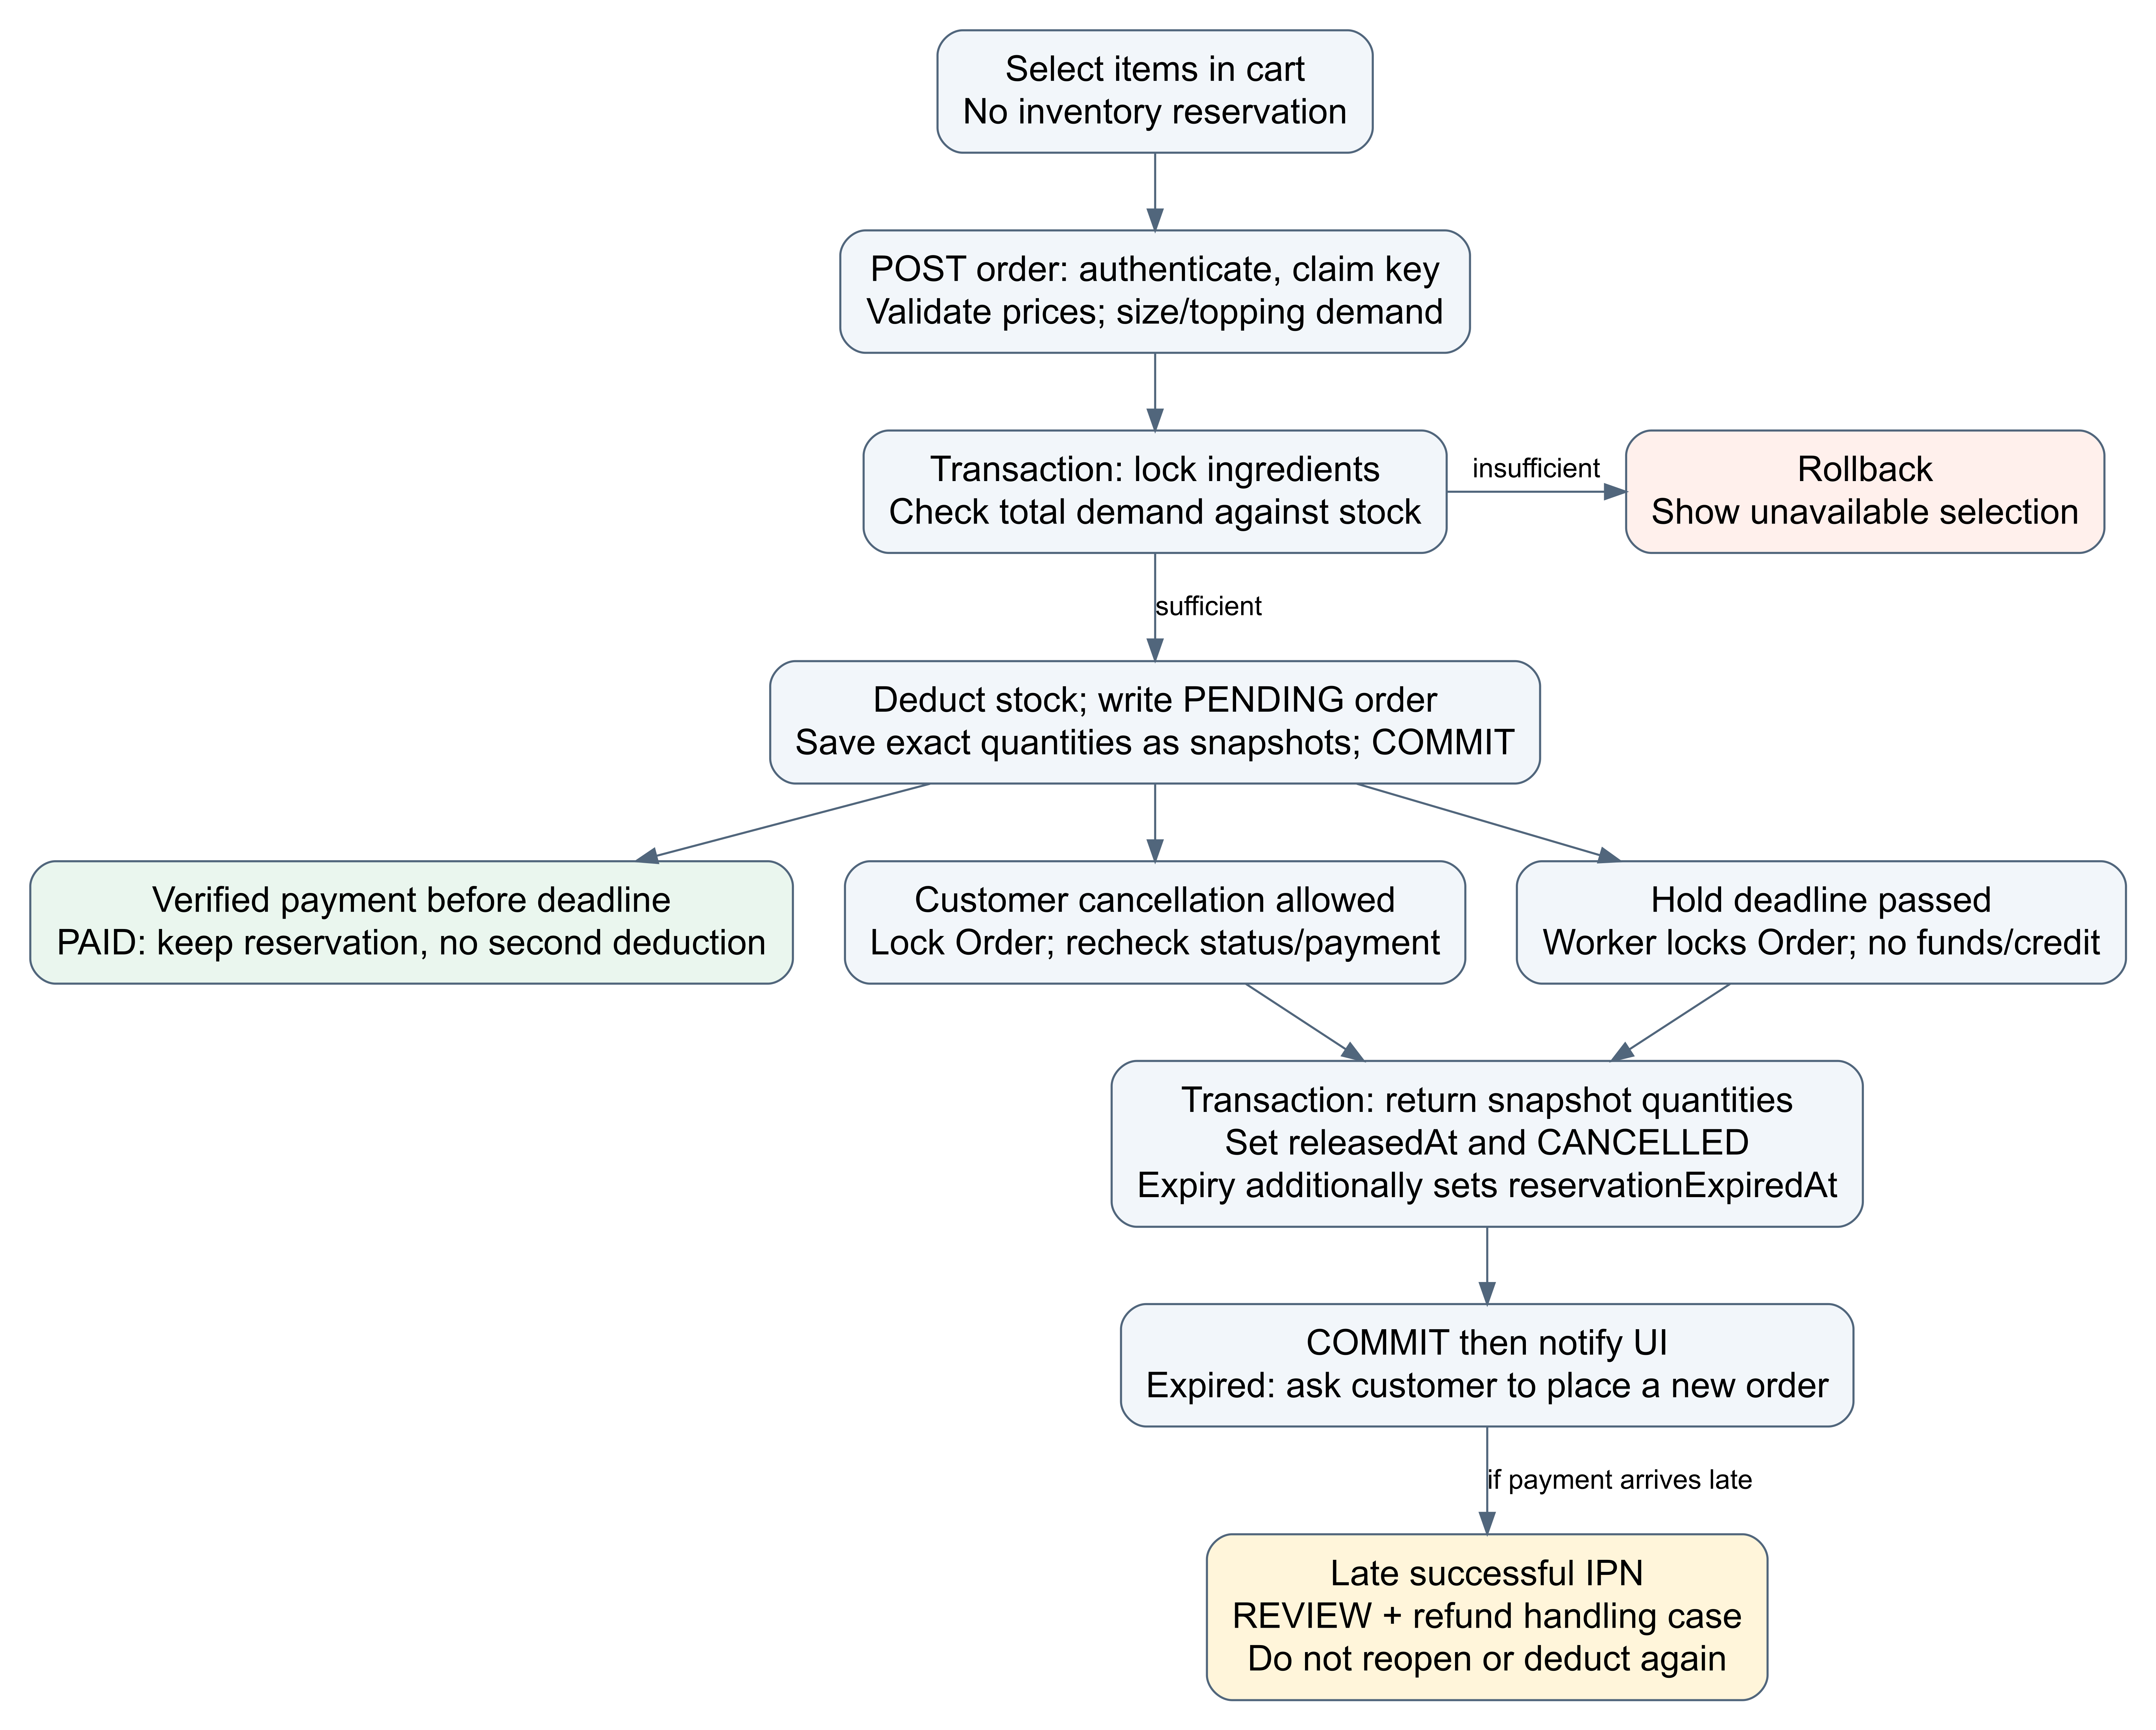
\includegraphics[width=\linewidth,height=.82\textheight,keepaspectratio]{assets/inventory/inventory-lifecycle.png}
\caption{Luồng tạo đơn, giữ kho, thanh toán, hủy và hết thời hạn giữ món}
\label{fig:inventory-lifecycle}
\end{figure}


\subsection{Đổi món, chuyển tiền và thanh toán chênh lệch}
\label{sec:exchange-design}
Đổi món là quy trình thay thế một đơn đã thanh toán trước khi pha chế, không phải khách tự hủy để nhận tiền. Khách mở liên kết hỗ trợ trên Order PAID, chọn lại món/size/topping qua menu và giỏ đổi riêng; backend báo giá, khách gửi lý do và quầy quyết định. Mở menu hoặc nhận báo giá không tự hoàn kho hay đóng đơn cũ.

\subsubsection{Dữ liệu yêu cầu và báo giá}
OrderExchange lưu sourceOrderId, replacementOrderId, items, reason, trạng thái, quyết định và version. Liên kết hai Order giữ được lịch sử trước/sau thay vì sửa trực tiếp các dòng món của đơn đã thu tiền. Unique(sourceOrderId, key) cùng requestHash bảo vệ gửi lặp yêu cầu.

quotedLines/quotedTotal lưu báo giá đã nhận khi yêu cầu được tạo. Frontend gửi expectedQuote để backend đối chiếu fingerprint của báo giá; nếu giá/trạng thái đổi trước lúc gửi, khách phải xem lại. Fingerprint là dấu vân tay đối chiếu dữ liệu, không phải chữ ký cổng thanh toán. Khi đã tạo yêu cầu, bước duyệt dùng thành tiền snapshot, tránh tính lại theo giá menu mới trong lúc khách chờ.

\begin{table}[htbp]\centering\small
\begin{tabularx}{\linewidth}{|p{.24\linewidth}|X|}\hline
\textbf{Trạng thái} & \textbf{Ý nghĩa và tác động}\\\hline
REQUESTED & Chờ quầy; đơn nguồn vẫn PAID và giữ nguyên liệu. Chặn chuyển PREPARING cho tới khi xử lý yêu cầu.\\\hline
APPROVED & Đã tạo đơn thay thế, chuyển credit và đóng đơn nguồn trong cùng transaction.\\\hline
REJECTED & Quầy từ chối, lưu ghi chú; giữ nguyên món và tiền của đơn nguồn.\\\hline
WITHDRAWN & Khách rút yêu cầu còn chờ bằng version; tiếp tục đơn nguồn.\\\hline
\end{tabularx}\caption{Vòng đời yêu cầu đổi món, độc lập vòng đời Order}
\end{table}

\subsubsection{Chuyển giá trị đã trả và thu chênh lệch}
Giá trị có thể chuyển bằng tổng Payment đã áp dụng của đơn nguồn cộng creditApplied đã chuyển vào đơn đó; backend kiểm bằng total của đơn nguồn trước khi duyệt. Credit là giá trị gắn với đơn thay thế, không phải số dư ví dùng tùy ý.

\begin{table}[htbp]\centering\small
\begin{tabularx}{\linewidth}{|X|c|c|c|}\hline
\textbf{Trường hợp} & \textbf{Tiền cũ} & \textbf{Món mới} & \textbf{Thu thêm}\\\hline
Đổi bằng giá & 45.000đ & 45.000đ & 0đ\\\hline
Đổi cao hơn & 45.000đ & 75.000đ & 30.000đ\\\hline
Đổi thấp hơn & 45.000đ & 40.000đ & Yêu cầu chọn lại\\\hline
\end{tabularx}\caption{Ví dụ credit và số tiền thu thêm khi đổi món}
\end{table}

Order mới giữ total bằng giá trị món, creditApplied bằng tiền chuyển, amountDue bằng phần chênh lệch. Đổi bằng giá tạo Order PAID nhưng không tạo Payment giả hoặc cộng điểm trên tiền cũ lần nữa. Đổi cao hơn tạo Order PENDING; VNPay chỉ thu phần chênh lệch và điểm tính trên tiền mới. Quy tắc hiện tại không áp voucher mới trong yêu cầu đổi; phần thu dương qua tích hợp VNPay phải từ 5.000đ. Quầy chỉ bắt đầu pha khi đơn thay thế đã đủ tiền.

\begin{figure}[htbp]\centering
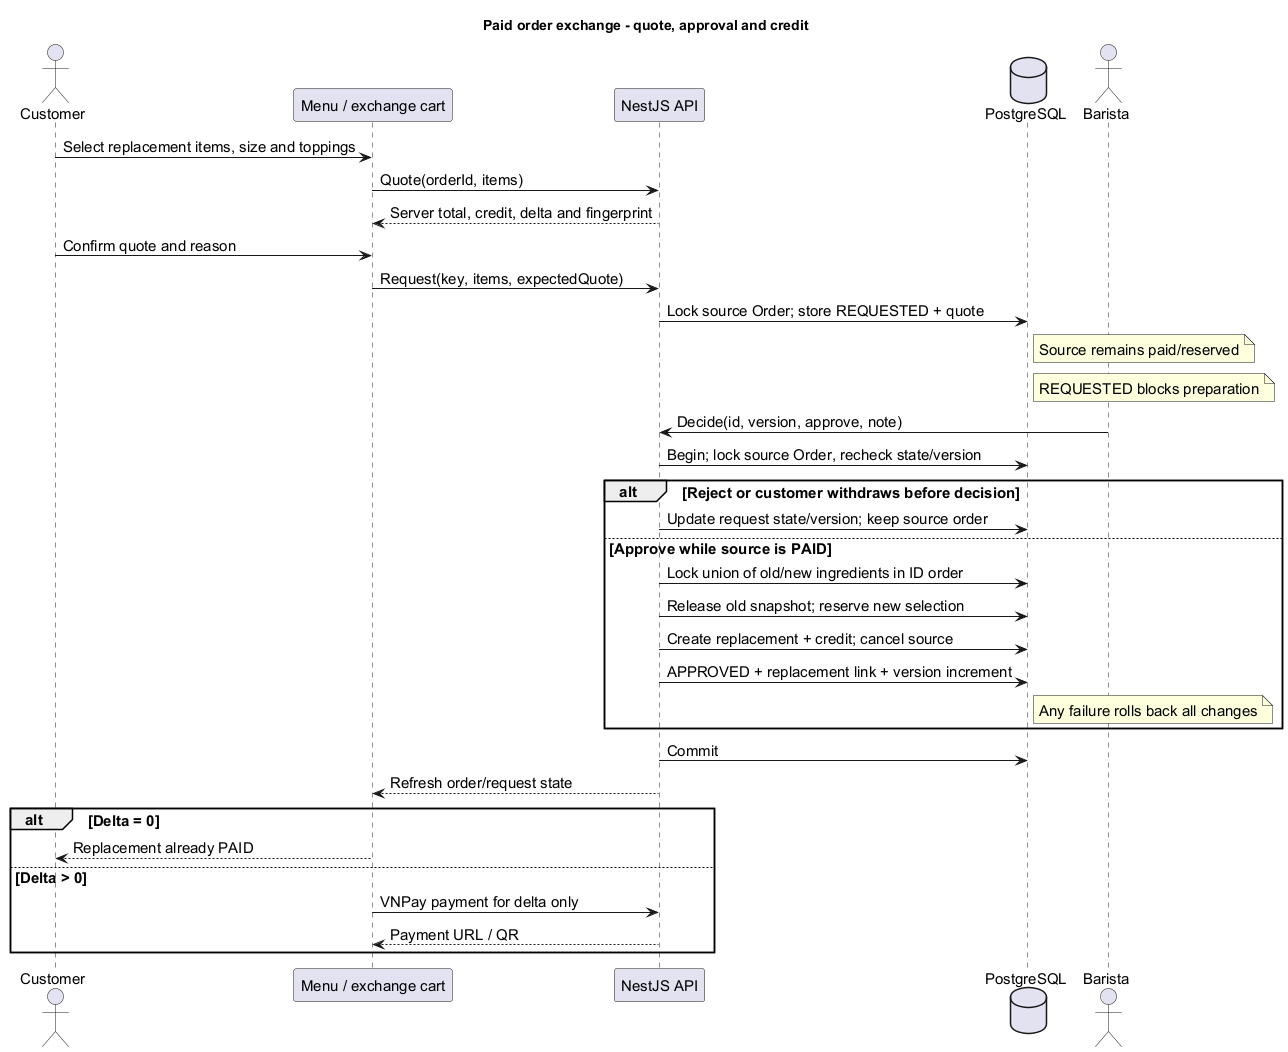
\includegraphics[width=\linewidth,height=.56\textheight,keepaspectratio]{assets/exchange/exchange-sequence.png}
\caption{Khách gửi yêu cầu, quầy quyết định, transaction thay đơn và thanh toán chênh lệch}
\end{figure}


\subsection{Version trong hồ sơ xử lý và khoản thu dư}
OrderExchange và PaymentRefundCase dùng version để phát hiện cập nhật trên dữ liệu cũ. Hai nhân viên cùng đọc version=0: người ghi trước cập nhật với điều kiện id/version/trạng thái rồi tăng lên 1; người còn lại bị 409. Đây là optimistic concurrency cho hồ sơ; việc giữ nguyên liệu sử dụng khóa dòng trong transaction.

PaymentRefundCase liên kết duy nhất với attempt đã thu nhưng không áp dụng được. Quy trình OPEN, PROCESSING, COMPLETED có ghi chú, người xử lý, thời gian và chứng từ duy nhất. Nhân viên thực hiện chuyển trả bên ngoài rồi ghi nhận bằng chứng; backend theo dõi bằng chứng từ và nhật ký xử lý. Thu trùng khác với khách đổi ý sau trả tiền và không bị ép sử dụng khoản dư để mua món khác.


\subsection{Mô hình hoạt động, tương tác và miền dữ liệu}
Ba hình dưới mô tả luồng đặt/thanh toán và mô hình miền ở mức chọn lọc, không thay thế kiểm thử hoặc chứng minh triển khai. Nguồn PlantUML và ảnh render được lưu cùng nhau tại \texttt{docs/diagrams/}. Voucher biểu diễn chính sách mã giảm giá; sổ LoyaltyTransaction lưu biến động điểm. Class diagram rút gọn thuộc tính, không phải bản sao đầy đủ schema.
\begin{figure}[p]\centering
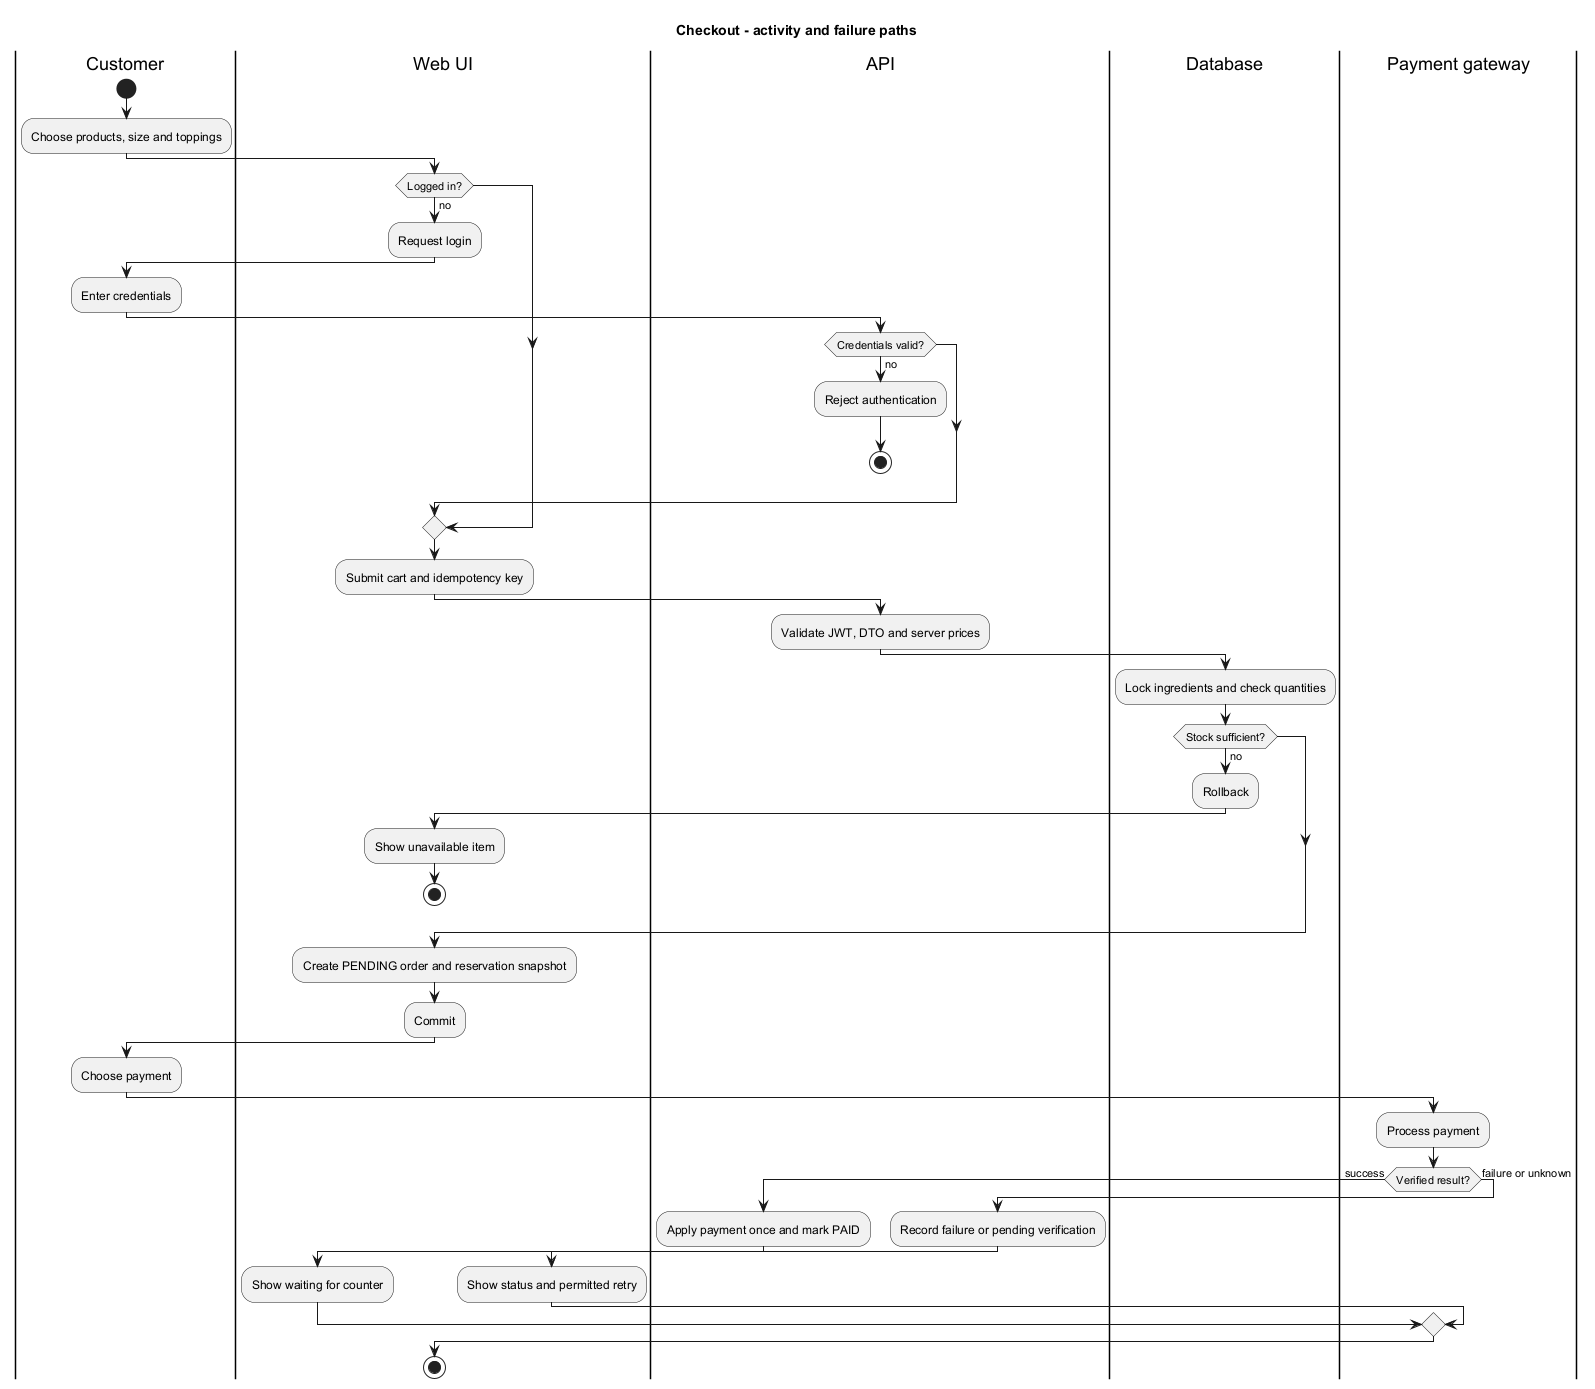
\includegraphics[width=\linewidth,height=.82\textheight,keepaspectratio]{../docs/diagrams/activity-checkout.png}
\caption{ACT-01: hoạt động đặt hàng với swimlane và nhánh chưa đăng nhập, hết kho, thanh toán lỗi}
\end{figure}
\begin{figure}[p]\centering
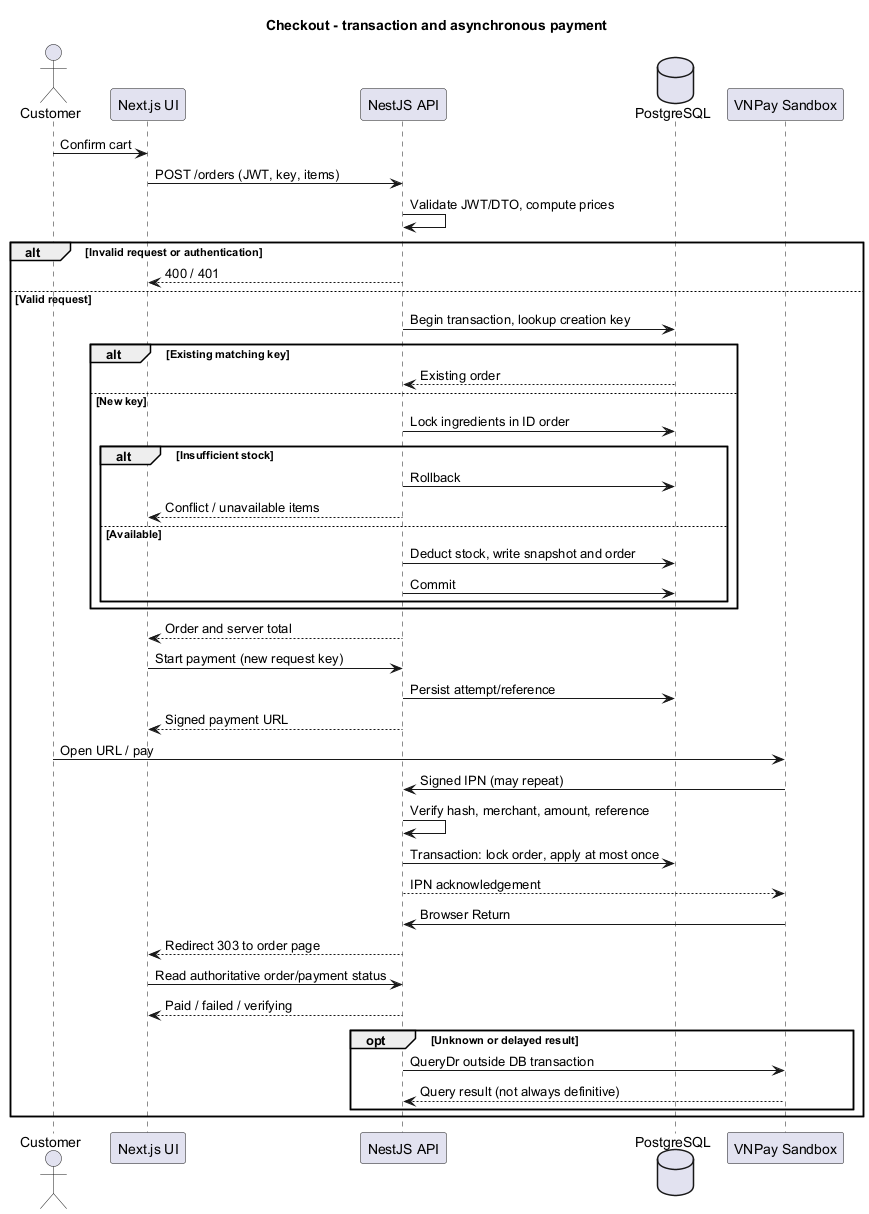
\includegraphics[width=\linewidth,height=.82\textheight,keepaspectratio]{../docs/diagrams/sequence-checkout.png}
\caption{SEQ-01: tương tác UI, API, database và gateway; transaction và callback bất đồng bộ}
\end{figure}
\begin{figure}[p]\centering
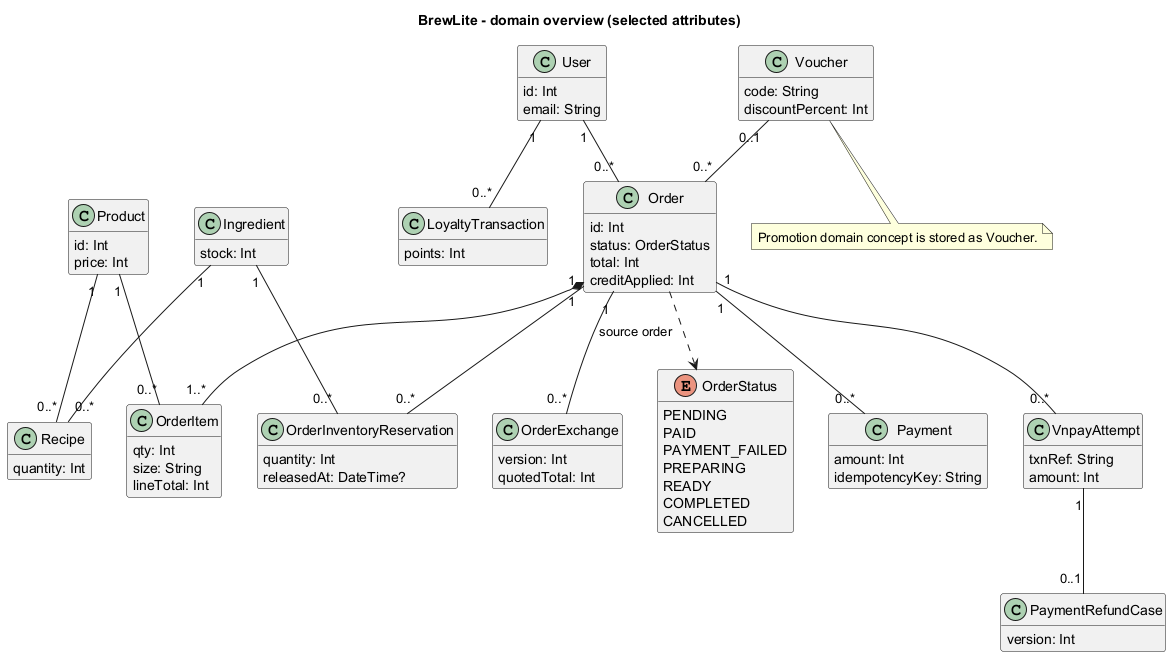
\includegraphics[width=\linewidth,height=.82\textheight,keepaspectratio]{../docs/diagrams/class-domain.png}
\caption{CLASS-01: các thực thể chính, quan hệ và bội số}
\end{figure}
\clearpage


\subsection{Thiết kế giao diện}
\label{sec:catalog-ui}
Menu ưu tiên tên món, giá và hình ảnh; trang chi tiết gom size, topping và số lượng trước thao tác thêm giỏ. Giỏ hàng cho sửa lựa chọn và xem tổng trước khi tạo đơn. Các màn hình thanh toán, đổi món và quầy được minh họa tại phần nghiệp vụ tương ứng.
\begin{figure}[htbp]\centering
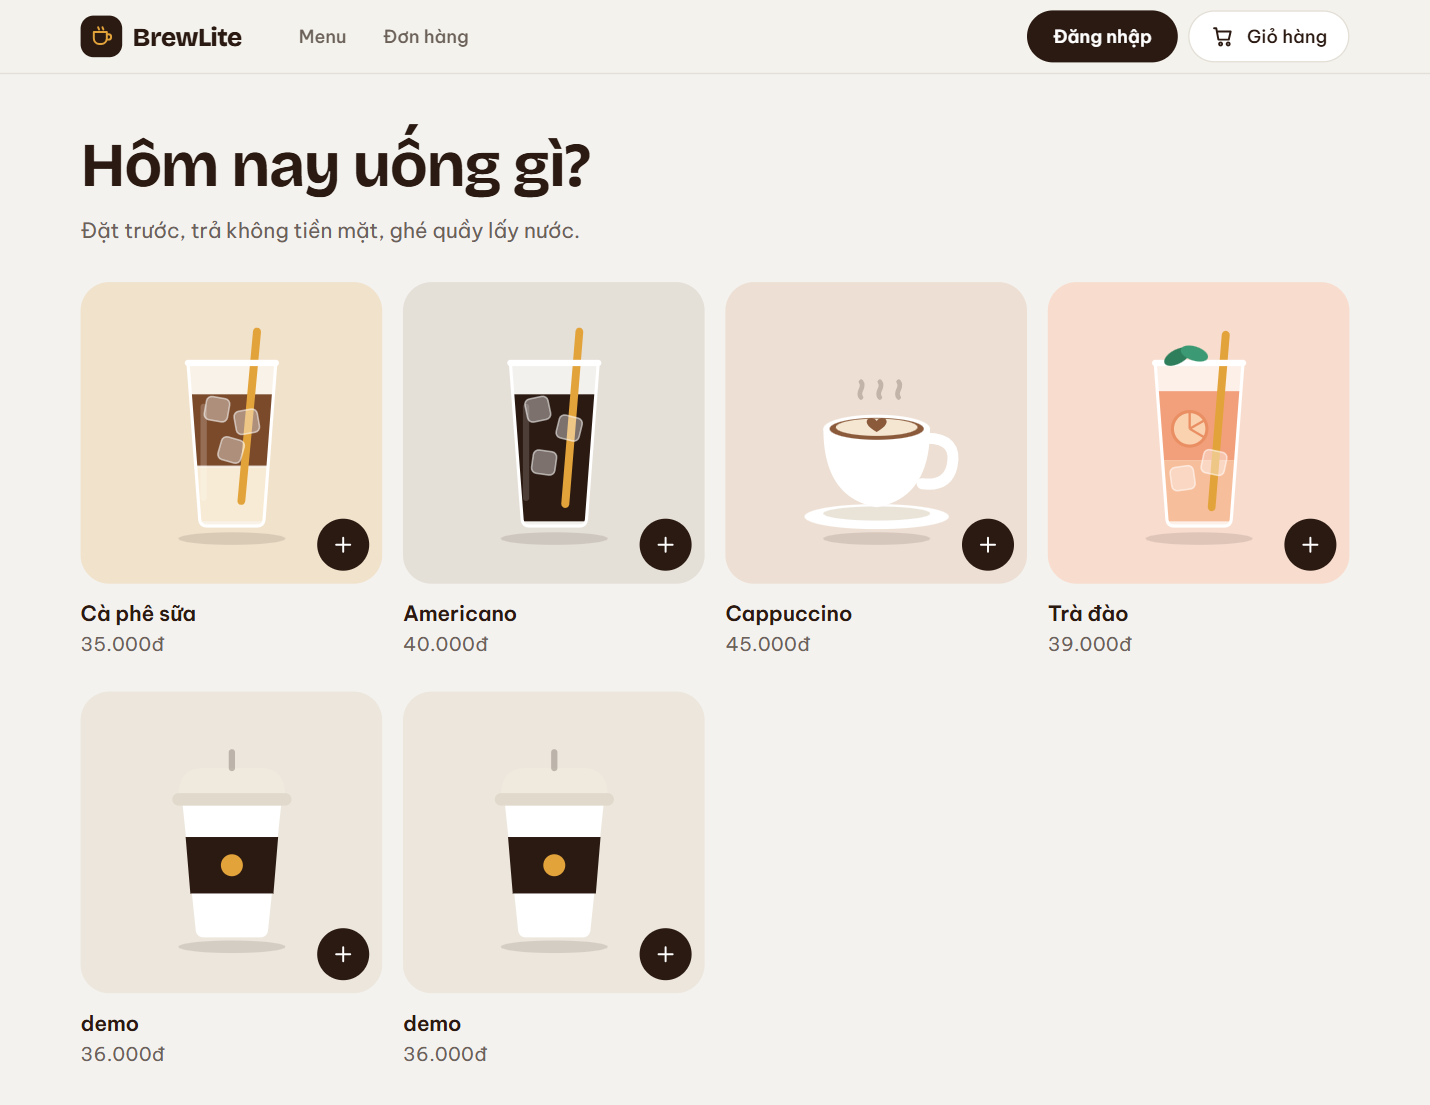
\includegraphics[width=.48\linewidth,height=.37\textheight,keepaspectratio]{assets/catalog-cart/ui-menu.png}\hfill
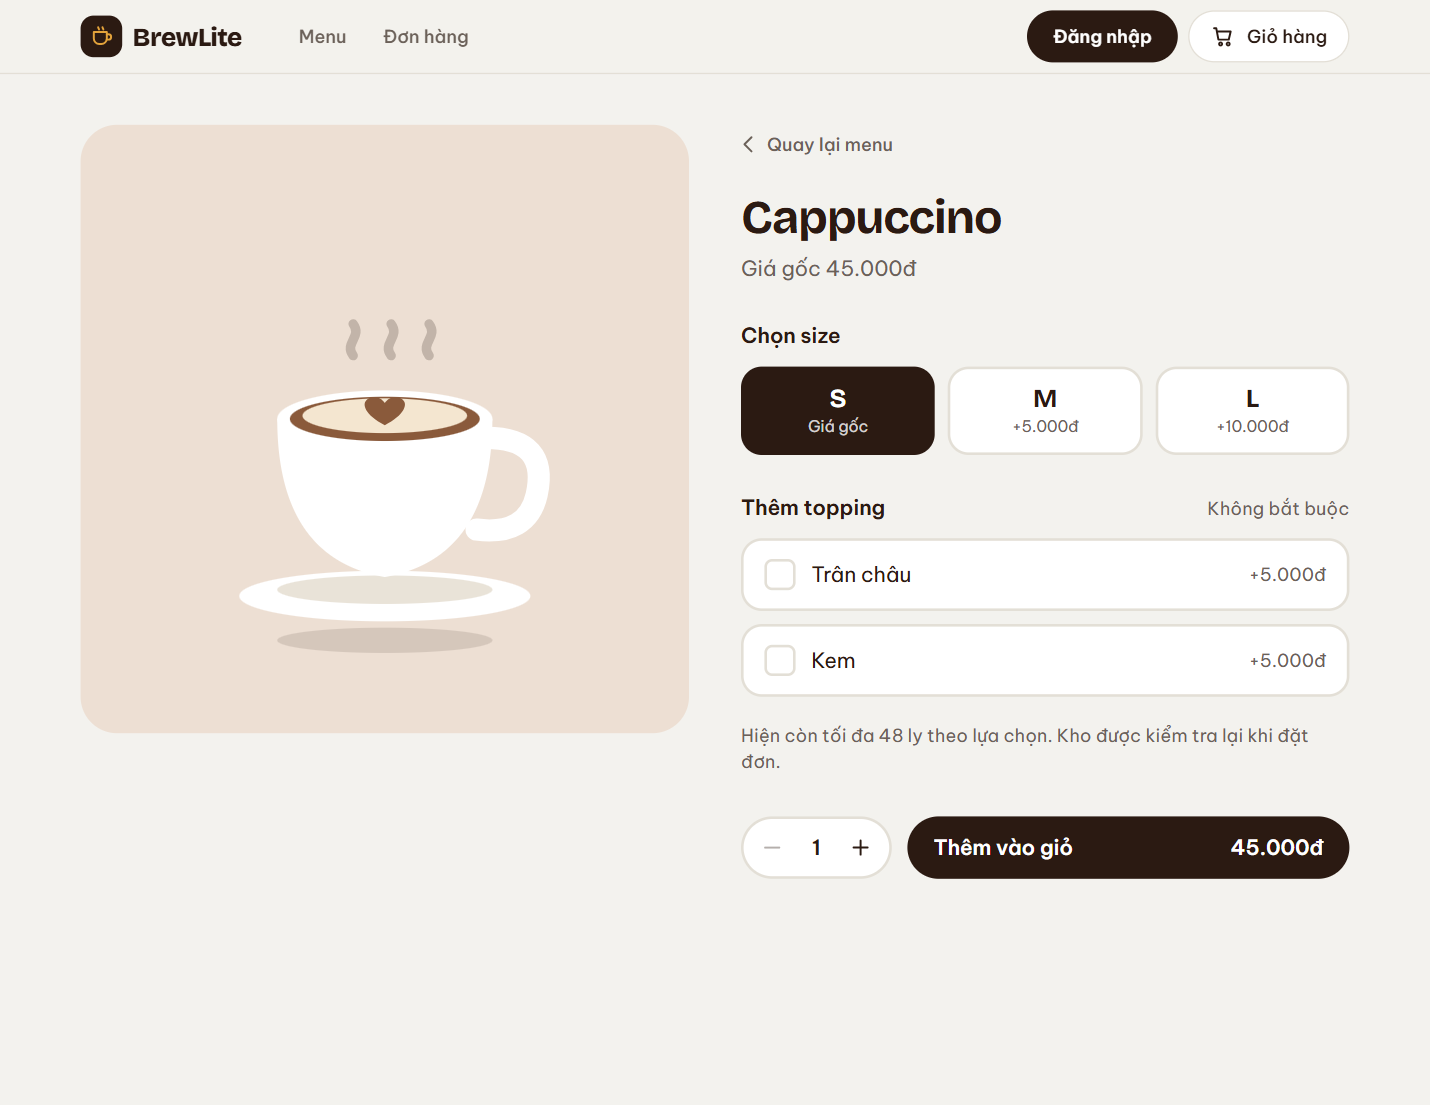
\includegraphics[width=.48\linewidth,height=.37\textheight,keepaspectratio]{assets/catalog-cart/ui-detail.png}
\caption{Menu và chi tiết món trên môi trường local, dùng API danh mục}
\vspace{3mm}
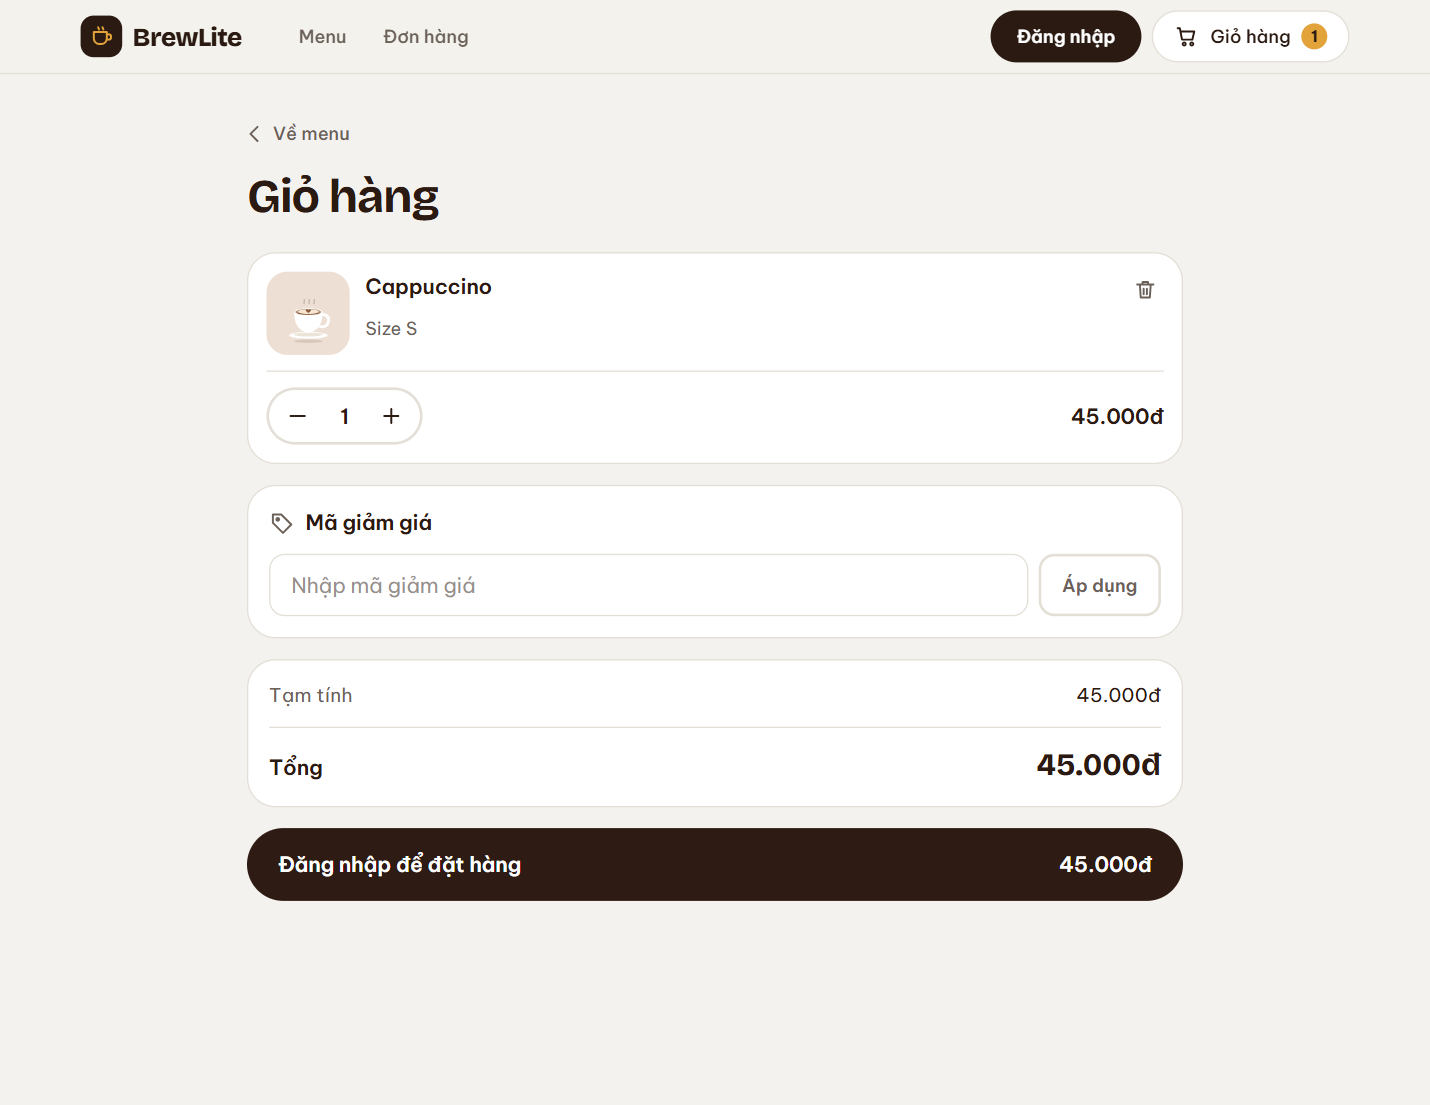
\includegraphics[width=.83\linewidth,height=.30\textheight,keepaspectratio]{assets/catalog-cart/ui-cart.png}
\caption{Giỏ hàng trước khi gửi đặt đơn; thao tác thêm món chỉ lưu ở trình duyệt}
\end{figure}

\newpage
%%%%%%%%%%%%%%%%%%%%%%%%%%%%%%%%%
\section{Hiện thực hệ thống}
\subsection{Cấu trúc thư mục}
\begin{lstlisting}[style=brew,language={}]
brewlite/
  docker-compose.yml
  README.md
  backend/             (NestJS)
    prisma/            schema, migrations, seed
    src/
      auth/  users/  products/  promotions/
      orders/  payments/  common/  prisma/
    test/              test end-to-end
  frontend/            (Next.js)
    src/
      app/             cac trang
      features/        auth, catalog, cart, orders, payments
      components/  lib/
\end{lstlisting}
Mỗi tính năng nằm trong thư mục riêng ở cả backend (module của NestJS) và frontend (thư mục \texttt{features}) để các thành viên ít đụng vào code của nhau.

\subsection{Menu, chi tiết sản phẩm và giỏ hàng}
\label{sec:catalog-cart}
\subsubsection{Tải menu và trạng thái giao diện}
MenuPage là Server Component gọi GET /products qua lớp API. ProductGrid hiển thị lưới responsive, ProductCard dẫn tới chi tiết theo id; danh sách rỗng có thông báo riêng, lỗi kết nối có nút tải lại. loading.tsx cung cấp khung chờ khi route tải dữ liệu. ProductImage dùng ảnh sản phẩm và minh họa dự phòng khi URL rỗng/ảnh lỗi, tránh đưa src rỗng vào thẻ img.

\subsubsection{Tùy chọn và giá hiển thị}
GET /products/:id cung cấp giá và danh mục phụ thu size/topping từ backend. ProductDetail giữ size, toppings, qty bằng state cục bộ, dùng calcUnitPrice để phản hồi ngay khi chọn. Ví dụ Cappuccino 45.000đ, size L thêm 10.000đ, một topping thêm 5.000đ thành 60.000đ. Availability theo tổ hợp hỗ trợ khóa lựa chọn thiếu nguyên liệu; đây là thông tin tại thời điểm đọc, không giữ hàng trong giỏ. Giá và lượng kho được backend kiểm lại khi tạo đơn như mục~\ref{sec:inventory-requirements}.

\subsubsection{State giỏ hàng và lưu qua lần tải lại}
Zustand lưu items, còn tổng tiền và badge được suy ra qua selector để không có nhiều bản sao tổng cần đồng bộ. Khóa dòng giỏ kết hợp productId, size và danh sách topping đã sort: cùng lựa chọn gộp số lượng, khác size/topping tách dòng. setQty cập nhật số lượng hoặc xóa khi về 0, giới hạn thao tác thông thường ở 99 ly/dòng.

persist lưu giỏ vào localStorage; useHydrated dùng snapshot server/client để tránh render số lượng lưu ở trình duyệt trước khi dữ liệu đó sẵn sàng. Đây là giỏ phía client theo origin, không phải một Order hoặc dữ liệu kho đã được giữ. Không tin unitPrice trong storage là giá thanh toán cuối.

\subsubsection{Gửi đặt hàng và khôi phục khi mất phản hồi}
CartView kiểm đăng nhập, chuyển tới login có next=/cart khi cần; khi đặt, chỉ gửi productId/size/topping/qty và mã voucher. placingRef chặn gửi chồng trong một component. prepareCheckoutIntent lưu key/nội dung theo tài khoản trong sessionStorage trước khi gửi: cùng nội dung sau mất phản hồi dùng lại key, không âm thầm tạo đơn mới. Backend idempotency vẫn là lớp bảo đảm như phần tạo đơn.

Chỉ sau response xác nhận Order, client xóa giỏ, hoàn tất intent và chuyển tới trang đơn. Nếu lỗi hoặc chưa rõ kết quả, giữ ý định để kiểm tra/retry phù hợp. SessionStorage không chứa token của intent; token đăng nhập được lớp auth quản lý riêng. Việc tính giá frontend hỗ trợ trải nghiệm, còn transaction backend chốt giá và giữ kho.

\begin{figure}[htbp]\centering
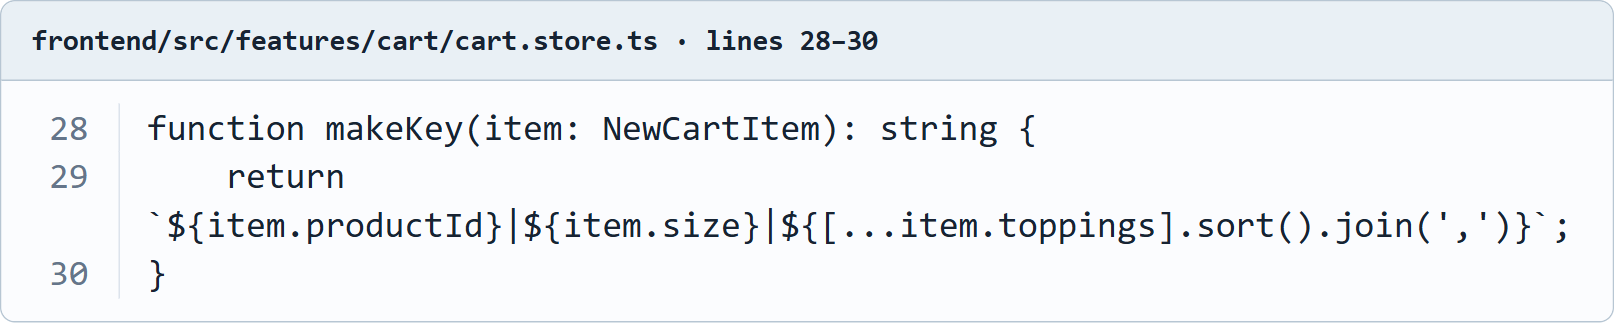
\includegraphics[width=.93\linewidth,height=.24\textheight,keepaspectratio]{assets/catalog-cart/code-key.png}
\caption{Khóa dòng giỏ được chuẩn hóa theo sản phẩm, size và topping}
\vspace{3mm}
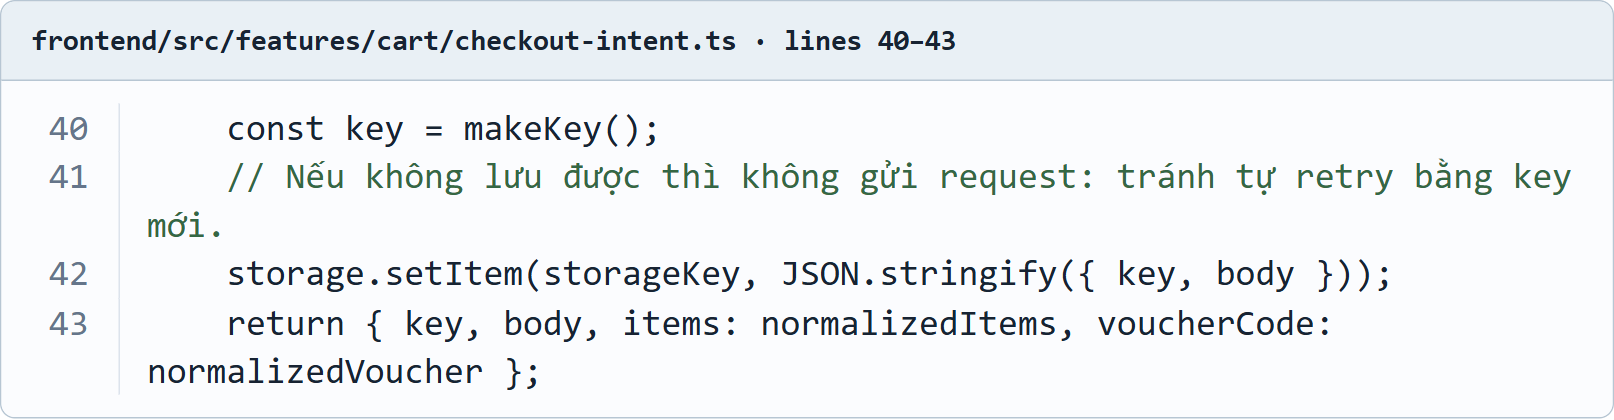
\includegraphics[width=.93\linewidth,height=.24\textheight,keepaspectratio]{assets/catalog-cart/code-intent.png}
\caption{Lưu ý định đặt hàng trước khi gửi để tái sử dụng key khi cần}
\vspace{3mm}
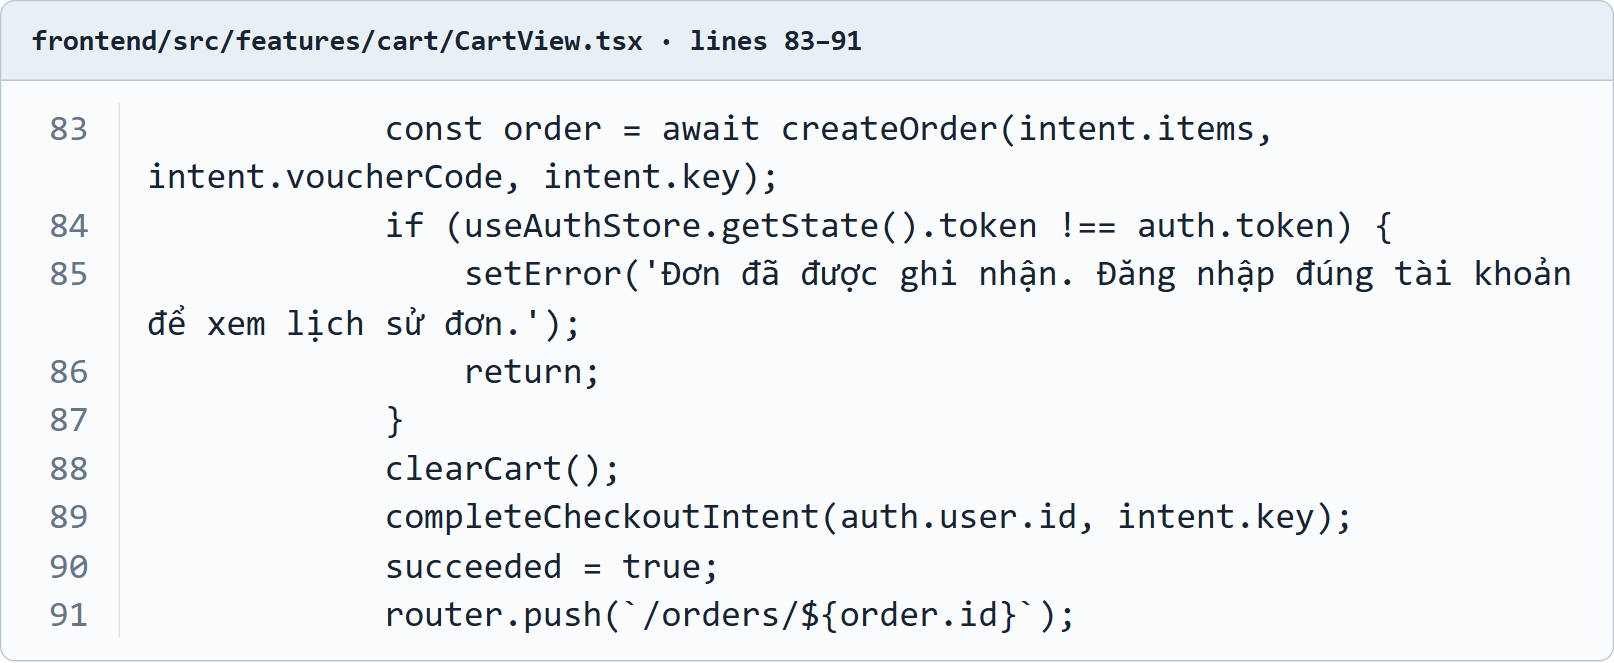
\includegraphics[width=.93\linewidth,height=.25\textheight,keepaspectratio]{assets/catalog-cart/code-submit.png}
\caption{Gửi lựa chọn và chỉ xóa giỏ sau khi backend xác nhận đơn}
\end{figure}


\subsection{Xác thực}
\label{sec:auth-implementation}
\subsubsection{Đăng ký, đăng nhập và dữ liệu công khai}
AuthService chuẩn hóa email bằng trim/lowercase. Đăng ký kiểm email, băm mật khẩu bằng bcrypt với cost 10 rồi tạo User CUSTOMER; đăng nhập dùng compare với hash đã lưu. Sai email hoặc mật khẩu trả cùng thông báo. UsersService dùng select các trường công khai khi tạo/đọc theo id; response không trả passwordHash.

AuthModule cấp access token thời hạn 7 ngày, payload nghiệp vụ gồm sub=id và email; thư viện quản lý trường thời gian. JWT được ký để kiểm chứng, không dùng như dữ liệu bí mật đã mã hóa. Secret lấy ở backend qua cấu hình môi trường. Frontend gửi token qua Authorization: Bearer khi gọi API được bảo vệ.

\subsubsection{Chuỗi kiểm tra JWT, vai trò và chủ đơn}
JwtAuthGuard dùng Passport strategy jwt để kiểm chữ ký và hạn. JwtStrategy.validate đọc lại User theo sub và trả id/email/role vào request.user; vì role lấy từ database ở mỗi lần validate, thay quyền có hiệu lực ở request xác thực tiếp theo mà không đợi token cũ hết hạn. CurrentUser chỉ trích request.user cho controller, không tự xác minh token lần nữa.

Route quầy khai báo UseGuards(JwtAuthGuard, RolesGuard) và Roles(BARISTA). RolesGuard đọc metadata của handler/class, đối chiếu role đã lấy từ database. Với route cá nhân, service còn kiểm userId của Order; có JWT đúng chưa đồng nghĩa được truy cập mọi mã đơn. Việc quyết định trạng thái, credit và version tiếp tục áp dụng sau khi qua lớp quyền.

\subsubsection{Trạng thái đăng nhập ở giao diện}
AuthForm gọi API, lưu accessToken/user vào Zustand persist và điều hướng về trang đang cần hoặc quầy theo role. Tham số next chỉ chấp nhận đường dẫn nội bộ để tránh điều hướng ra website tùy ý. Auth store hiện lưu qua localStorage; logout xóa trạng thái ở trình duyệt. Đây là thao tác kết thúc phiên phía client, không được hiểu là đã thu hồi mọi JWT đã phát hành. Dữ liệu role trên UI phục vụ hiển thị; backend vẫn quyết định quyền thật.

\begin{figure}[htbp]\centering
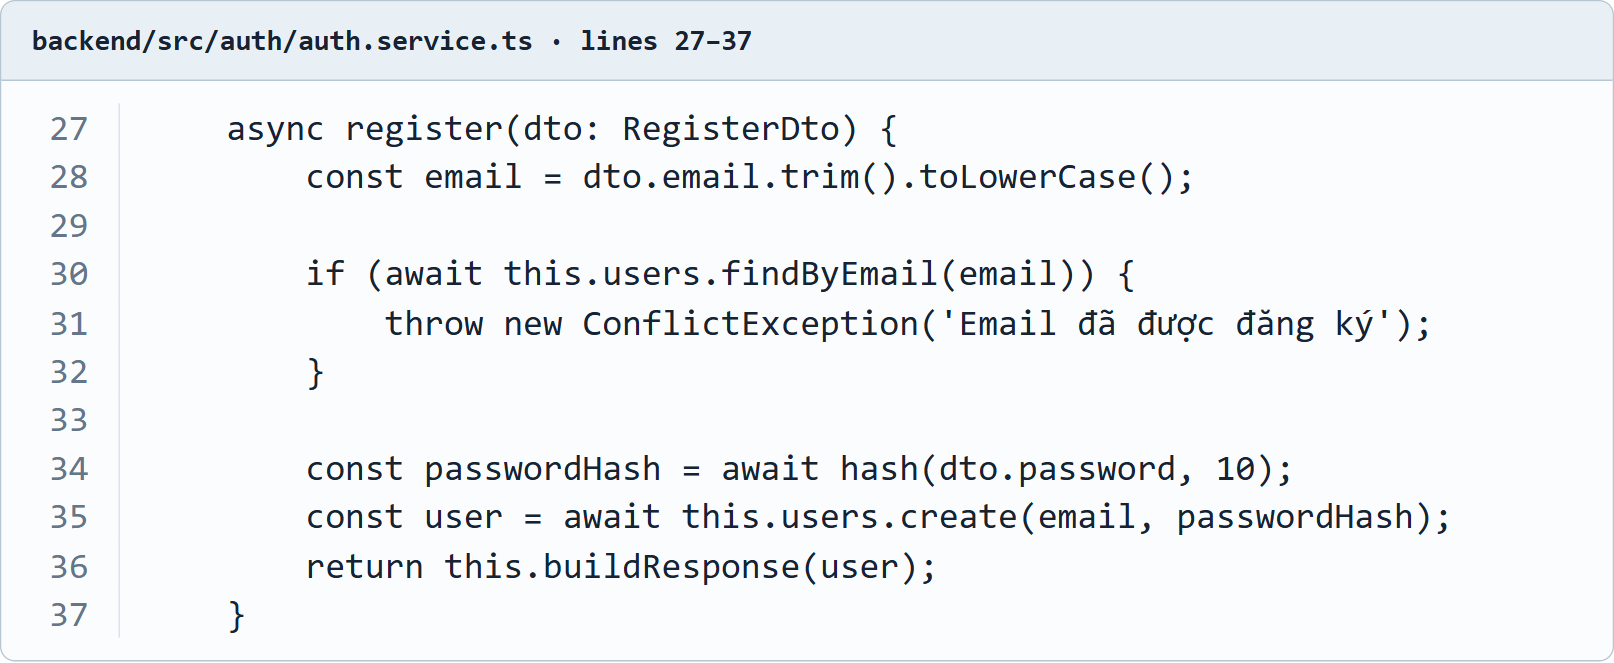
\includegraphics[width=.94\linewidth,height=.23\textheight,keepaspectratio]{assets/auth/code-register.png}
\caption{Đăng ký chuẩn hóa email và lưu hash thay vì mật khẩu gốc}
\vspace{3mm}
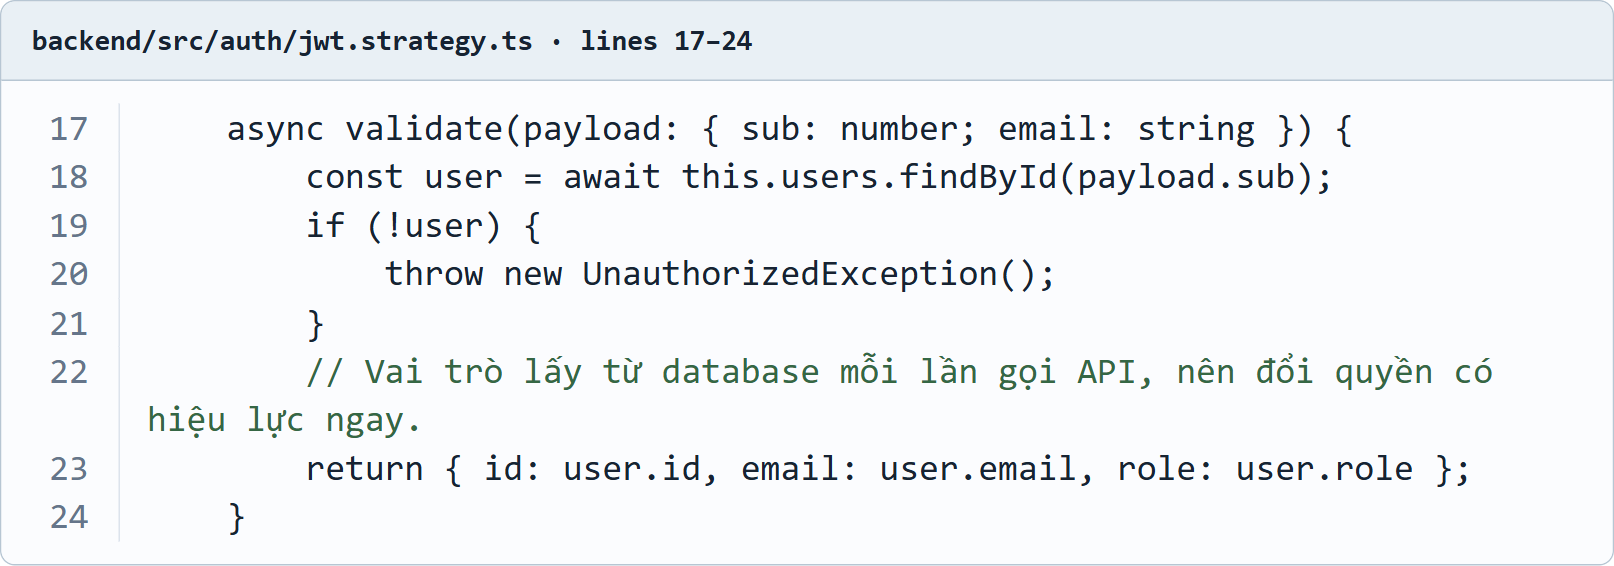
\includegraphics[width=.94\linewidth,height=.23\textheight,keepaspectratio]{assets/auth/code-strategy.png}
\caption{JWT strategy lấy vai trò hiện tại từ User trong database}
\vspace{3mm}
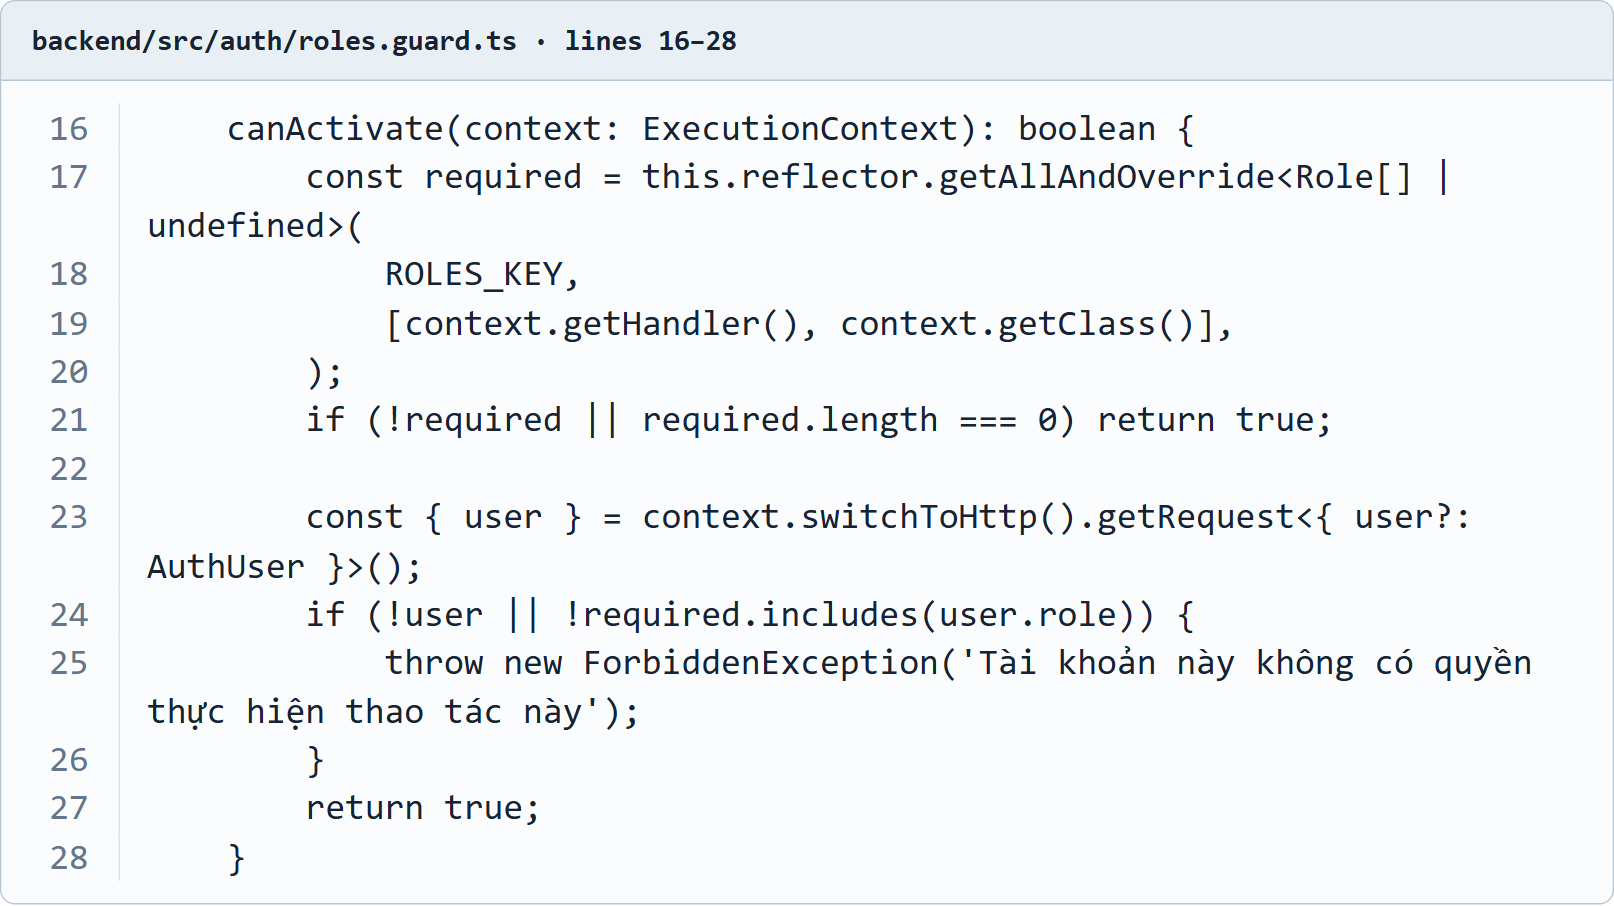
\includegraphics[width=.94\linewidth,height=.25\textheight,keepaspectratio]{assets/auth/code-role.png}
\caption{RolesGuard đối chiếu vai trò với metadata của route}
\end{figure}


\subsection{Tạo đơn và tích hợp thanh toán}
\texttt{POST /orders} nhận danh sách món (mã sản phẩm, size, topping, số lượng), tự lấy giá từ cơ sở dữ liệu, tính lại tổng tiền và lưu đơn PENDING. Giá do trình duyệt gửi lên không được tin.

Cổng giả lập dùng để kiểm tra luồng Ví/Thẻ có kiểm soát; khi bật VNPay, endpoint mock bị chặn để không bỏ qua cổng. Luồng VNPay tách quá trình khách thao tác ở cổng khỏi transaction ghi nhận kết quả tại backend.

\subsubsection{Hiện thực VNPay và bảo đảm ghi nhận một lần}
\label{sec:vnpay-implementation}
VnpayGateway chịu trách nhiệm cấu hình, build URL và QueryDr. Các hàm canonical/hmac/readCallback tách xử lý chữ ký khỏi nghiệp vụ. VnpayService.start/replay kiểm yêu cầu bắt đầu; ipn/returnUrl phân biệt hai kênh; apply ghi nhận kết quả; check điều phối đối soát theo yêu cầu. Frontend PaymentQr/VnpayPanel chỉ hiển thị và gọi API.

\paragraph{Xác minh trước khi ghi.}
Callback phải có dạng dữ liệu hợp lệ; canonical loại trường hash, sắp khóa và encode một lần; HMAC so bằng timingSafeEqual sau kiểm độ dài/định dạng. Chữ ký đúng vẫn phải kiểm merchant, txnRef, amount và mã trạng thái. Nhóm không xem chữ ký như mã hóa nội dung hoặc bằng chứng rằng đơn chắc chắn còn được phục vụ. QueryDr ký theo chuỗi trường của giao thức riêng, không dùng lại querystring của URL thanh toán.

\paragraph{Transaction và idempotency.}
apply khóa Order trước, đọc lại attempt và kiểm paidAt/khoản đã áp dụng. Với kết quả thành công, chỉ canFulfill khi đơn payable còn hạn, số tiền khớp và snapshot còn giữ. Payment, Order PAID, điểm và nhật ký cùng transaction; lỗi ở bước cộng điểm rollback cả settlement. Key của Payment theo txnRef, unique providerTxnNo và liên kết attempt là các lớp kiểm soát bổ sung; khóa Order điều phối cả hai attempt khác nhau của cùng đơn.

\paragraph{Không giữ khóa trong lúc chờ mạng.}
QueryDr thực hiện ngoài transaction, có timeout 8 giây. lastCheckedAt được cập nhật có điều kiện để hạn chế tra cứu dồn trong khoảng 15 giây; đây là điều tiết truy vấn, không phải kết quả tài chính. Khi response được xác minh, apply lấy khóa và kiểm lại điều kiện tại thời điểm ghi. HTTP 200 của endpoint IPN chỉ xác nhận HTTP có phản hồi; mã RspCode trong JSON mới là ACK nghiệp vụ, không thay thế trạng thái Order/Payment.

\begin{figure}[htbp]\centering
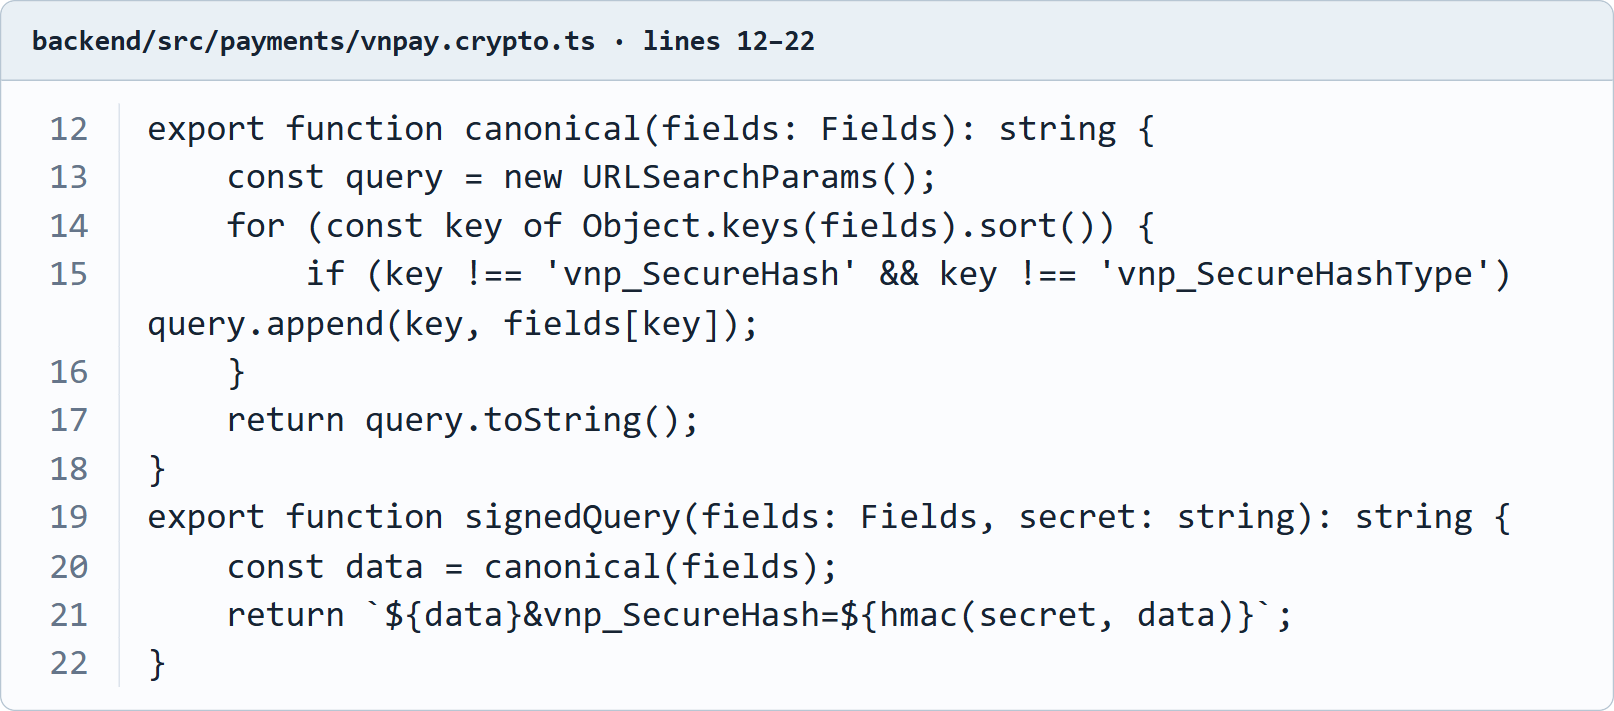
\includegraphics[width=.94\linewidth,height=.28\textheight,keepaspectratio]{assets/vnpay/code-canonical.png}
\caption{Chuẩn hóa tham số và ký URL trong vnpay.crypto.ts}
\vspace{4mm}
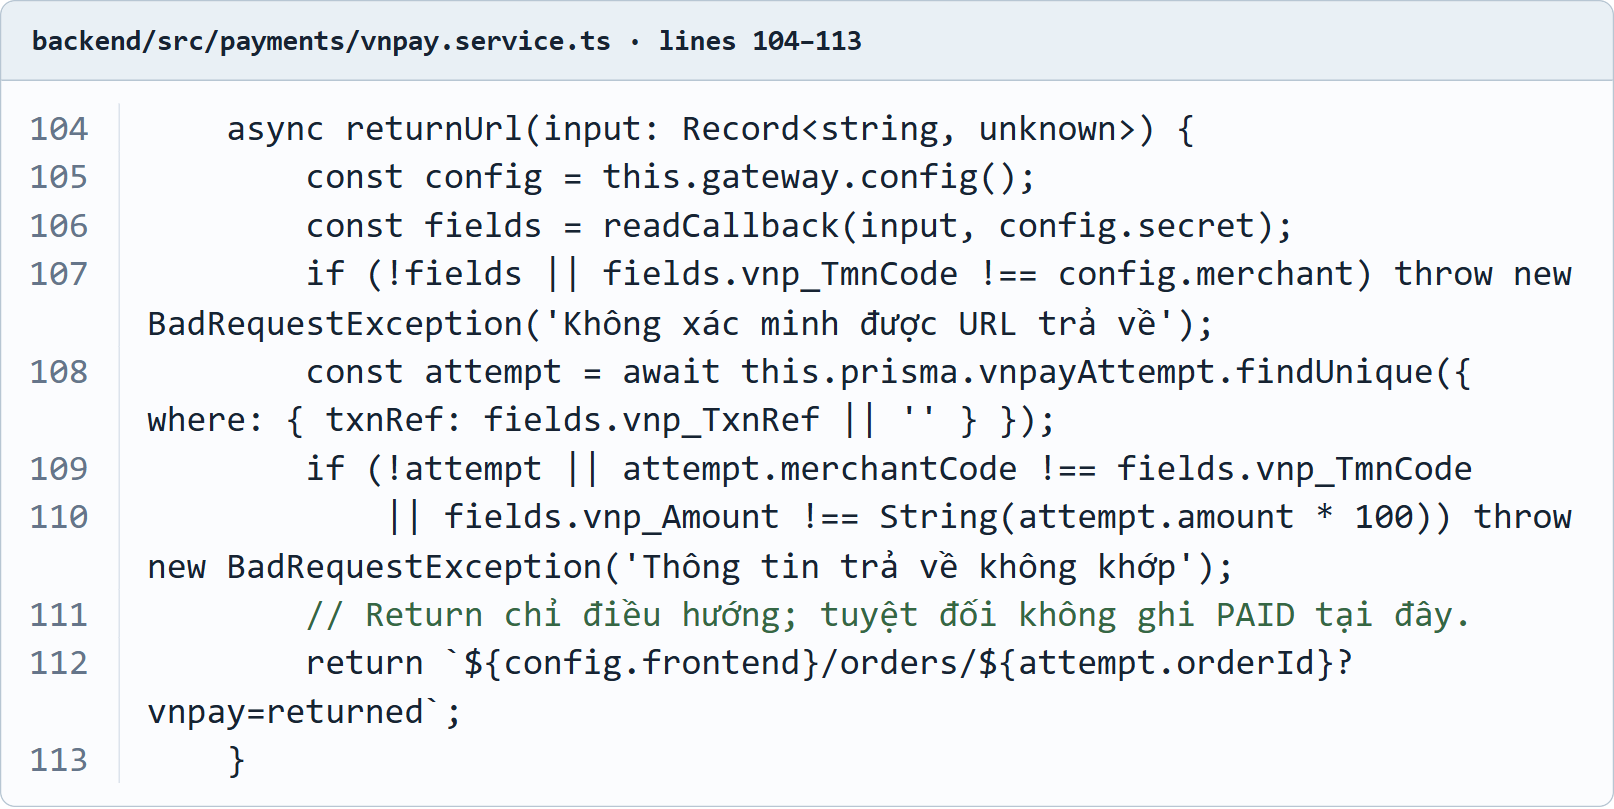
\includegraphics[width=.94\linewidth,height=.28\textheight,keepaspectratio]{assets/vnpay/code-return.png}
\caption{Return kiểm chứng dữ liệu rồi chỉ tạo đích chuyển hướng}
\end{figure}
\begin{figure}[htbp]\centering
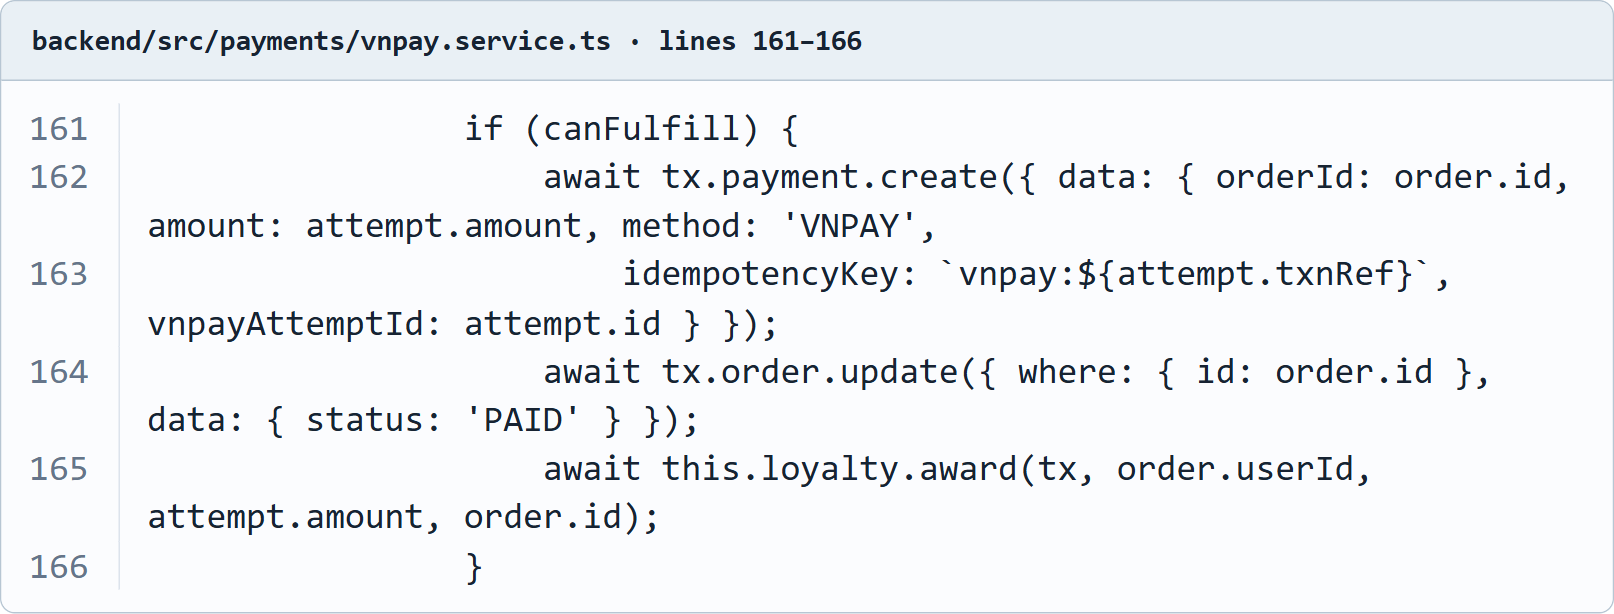
\includegraphics[width=.94\linewidth,height=.30\textheight,keepaspectratio]{assets/vnpay/code-settlement.png}
\caption{Nhánh canFulfill ghi Payment, PAID và điểm trong transaction apply}
\end{figure}


\subsection{Toàn vẹn đơn hàng, thanh toán và tồn kho}
\subsubsection{Order State Machine}
Bảng chuyển trạng thái hợp lệ nằm trong một tệp riêng, không phụ thuộc cơ sở dữ liệu nên kiểm thử được độc lập.
\begin{lstlisting}[style=brew]
export const ORDER_TRANSITIONS = {
  PENDING: ['PAID', 'PAYMENT_FAILED', 'CANCELLED'],
  PAYMENT_FAILED: ['PENDING', 'PAID', 'CANCELLED'],
  PAID: ['PREPARING', 'CANCELLED'],
  PREPARING: ['READY'],
  READY: ['COMPLETED'],
  COMPLETED: [],
  CANCELLED: [],
};

export function assertTransition(from, to) {
  if (!canTransition(from, to)) {
    throw new ConflictException('Khong the chuyen don tu ' + from + ' sang ' + to);
  }
}
\end{lstlisting}

\subsubsection{Thanh toán idempotent}
Mỗi yêu cầu thanh toán kèm header \texttt{Idempotency-Key}. Cùng một khóa chỉ được xử lý một lần; các lần sau trả lại kết quả của lần đầu, nên khách bấm nhiều lần hoặc mạng chập chờn cũng không ghi nhận khoản thanh toán hai lần bởi cùng một yêu cầu. Toàn bộ thanh toán chạy trong một giao dịch cơ sở dữ liệu. Dòng đơn hàng được khóa bằng \texttt{SELECT ... FOR UPDATE} để hai yêu cầu cùng một đơn phải xếp hàng, nhờ đó cổng thanh toán chỉ bị gọi một lần. Cột \texttt{idempotencyKey} duy nhất trong bảng Payment là chốt chặn cuối cùng.
\begin{lstlisting}[style=brew]
await tx.$queryRaw`SELECT id FROM "Order"
                   WHERE id = ${dto.orderId} FOR UPDATE`;
const replay = await this.findReplay(tx, userId, key, dto.orderId);
if (replay) return replay;   // cung Idempotency-Key: tra ket qua cu
\end{lstlisting}

\subsubsection{Kiểm soát tồn kho khi đặt đồng thời}
Khi nhiều khách cùng đặt món sử dụng chung nguyên liệu, backend phải bảo đảm tổng lượng giữ thành công không vượt tồn kho. Hệ thống tính nhu cầu theo size/topping, khóa các dòng Ingredient theo thứ tự id tăng dần, kiểm tra đủ lượng rồi mới trừ trong cùng transaction tạo Order và snapshot. Khách gửi lại cùng yêu cầu không bị giữ kho lần hai; hủy hợp lệ hoặc hết thời hạn giữ món sẽ hoàn đúng lượng đã lưu, không tính lại từ công thức hiện tại. Các phần dưới trình bày trách nhiệm từng hàm, cơ chế phối hợp và ảnh code hiện thực.
\paragraph{Tổ chức các hàm và ranh giới transaction.}
\label{sec:inventory-implementation}
\begin{longtable}{|p{.33\linewidth}|p{.58\linewidth}|}
\hline\textbf{Hàm/thành phần} & \textbf{Trách nhiệm}\\\hline\endhead
OrdersService.create & Xác lập quyền sở hữu idempotency key, tính giá/voucher, gọi reserve, tạo Order/OrderItem/snapshot và gắn kết quả vào key trong một transaction.\\\hline
ingredientDemand & Chuyển lựa chọn món/size/topping thành tổng lượng theo ingredientId; kiểm tra định lượng và giới hạn số nguyên.\\\hline
InventoryService.reserve & Đọc công thức, tính demand, khóa Ingredient theo id tăng dần, kiểm đủ toàn bộ rồi trừ; trả lượng đã trừ để lưu snapshot.\\\hline
OrdersService.cancel & Kiểm tra quyền/trạng thái, khóa Order, kiểm tra thanh toán, cập nhật CANCELLED có điều kiện và gọi release.\\\hline
InventoryService.release & Khóa snapshot theo đơn; chặn thiếu snapshot/đã hoàn; cộng lại quantity và ghi releasedAt trong transaction do hàm gọi cung cấp.\\\hline
ReservationExpiryService & Tìm đơn quá hạn đủ điều kiện, lấy khóa không chờ trên đơn, kiểm lại sau khóa, release và đóng đơn; phát thông báo sau commit.\\\hline
ExchangeService.decide & Khi duyệt đổi, khóa Order cũ và tập nguyên liệu liên quan, hoàn snapshot cũ, giữ lựa chọn mới và tạo đơn thay thế trong cùng transaction.\\\hline
\caption{Phân trách nhiệm để tái sử dụng và kiểm thử độc lập}
\end{longtable}

\paragraph{Tính nguyên tử.}
Giả sử đơn có cà phê và trà: cà phê còn đủ nhưng trà hết. Backend không được tạo một nửa Order hoặc giữ riêng phần cà phê. Transaction làm cho thao tác hoặc commit toàn bộ hoặc rollback toàn bộ. Tương tự, hủy đơn không được commit trạng thái CANCELLED nhưng bỏ quên bước hoàn nguyên liệu. Snapshot, kho và trạng thái phải cùng commit.

\paragraph{Chống gửi lặp trước khi chạm kho.}
Unique key theo khách trong OrderCreateRequest được xác lập trước reserve. Hai request cùng key cùng nội dung sẽ quy về một Order; key cũ với nội dung khác bị từ chối. Vô hiệu hóa nút frontend chỉ hỗ trợ thao tác, còn ràng buộc database mới bảo vệ khi request bị gửi lại hoặc có nhiều tab/process. Khi một transaction tranh key thất bại, backend rollback rồi đọc kết quả đã lưu, không tiếp tục truy vấn trong transaction đang lỗi.

\paragraph{Chống tranh phần cuối bằng khóa dòng.}
Reserve dùng SELECT FOR UPDATE trên các Ingredient cần dùng. Nếu A và B cùng cần 20g cuối, A lấy khóa trước, kiểm đủ rồi trừ về 0 và commit. B chờ khóa; khi được xử lý, B thấy tồn 0 nên bị từ chối. Khóa chỉ giữ trong transaction ngắn; không giữ trong lúc khách chọn món hoặc mở trang VNPay. Database còn có CHECK stock không âm như lớp bảo vệ dữ liệu.

Khóa theo id tăng dần giúp các transaction lấy nhiều nguyên liệu theo cùng thứ tự. Ví dụ cả A và B đều lấy nguyên liệu 1 rồi 2, tránh tình huống mỗi bên giữ một nguyên liệu rồi chờ nguyên liệu của bên kia. Các luồng thanh toán/hủy/hết hạn cùng lấy khóa Order trước để kiểm tra trạng thái nhất quán.

\paragraph{Hoàn đúng một lần.}
Hai yêu cầu hủy cùng Order phải qua khóa Order và cập nhật trạng thái có điều kiện. Chỉ giao dịch thực sự chuyển được trạng thái mới release. Bên trong release, snapshot tiếp tục được khóa và releasedAt được kiểm tra. Hai lớp này bảo vệ cả API hủy lẫn việc gọi lại hàm release; lỗi sau khi cộng kho vẫn rollback cả dấu hoàn.

\paragraph{Nhiều worker và thông báo.}
Cờ running tránh hai lượt quét chồng trong một process. SELECT FOR UPDATE SKIP LOCKED mới là cơ chế phối hợp ở database khi nhiều worker cùng xử lý một đơn: bên chưa lấy được khóa bỏ qua, không xử lý trùng. Sau khi lấy khóa, worker đọc lại trạng thái và bằng chứng nhận tiền. Thông báo orders.changed phát sau commit; UI tải lại dữ liệu và có polling HTTP 15 giây khi tab hiển thị. Tác vụ quét tiếp tục khi backend khởi động lại vì deadline nằm trong database.

\paragraph{Kết hợp khóa dòng và kiểm tra phiên bản.}
Kho và vòng đời Order dùng khóa dòng. OrderExchange và PaymentRefundCase dùng thêm cập nhật có điều kiện theo version: chỉ ghi khi id/version/trạng thái còn khớp, rồi tăng version; cập nhật không tác động một dòng trả lỗi xung đột. Ví dụ hai barista cùng đọc version=0 thì người ghi sau không thể ghi đè quyết định đã nâng lên version=1. Mỗi cơ chế gắn với đối tượng nghiệp vụ cụ thể.

\begin{figure}[p]\centering
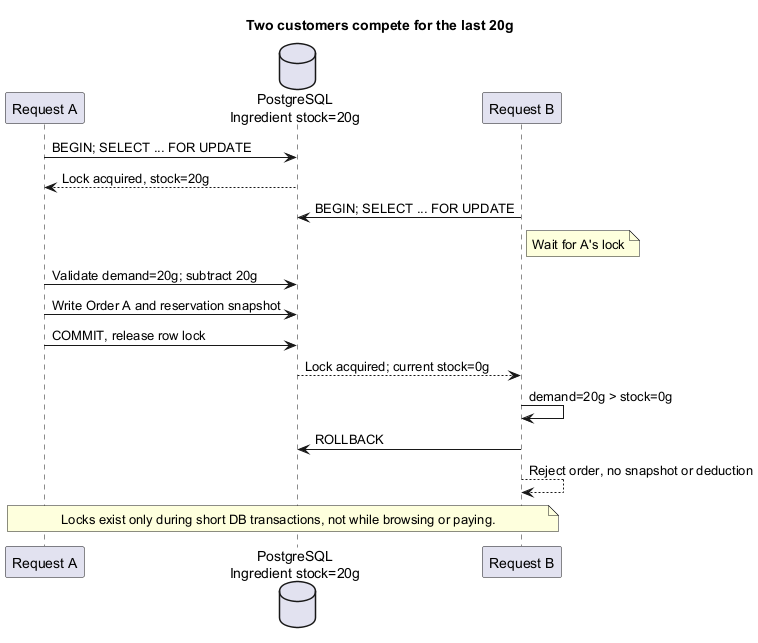
\includegraphics[width=\linewidth,height=.78\textheight,keepaspectratio]{assets/inventory/inventory-concurrency.png}
\caption{Hai khách tranh phần nguyên liệu cuối: chỉ transaction đủ kho được commit}
\end{figure}

\paragraph{Ảnh chụp code từ phiên bản hiện thực.}
Các hình sau được chụp từ mã nguồn hiện tại; tên tệp và số dòng nằm trên ảnh để truy vết. Phần giải thích đọc cùng các hàm gọi bên ngoài: reserve/release nhận TransactionClient, nên ranh giới commit/rollback do service gọi quản lý.

\begin{figure}[p]\centering
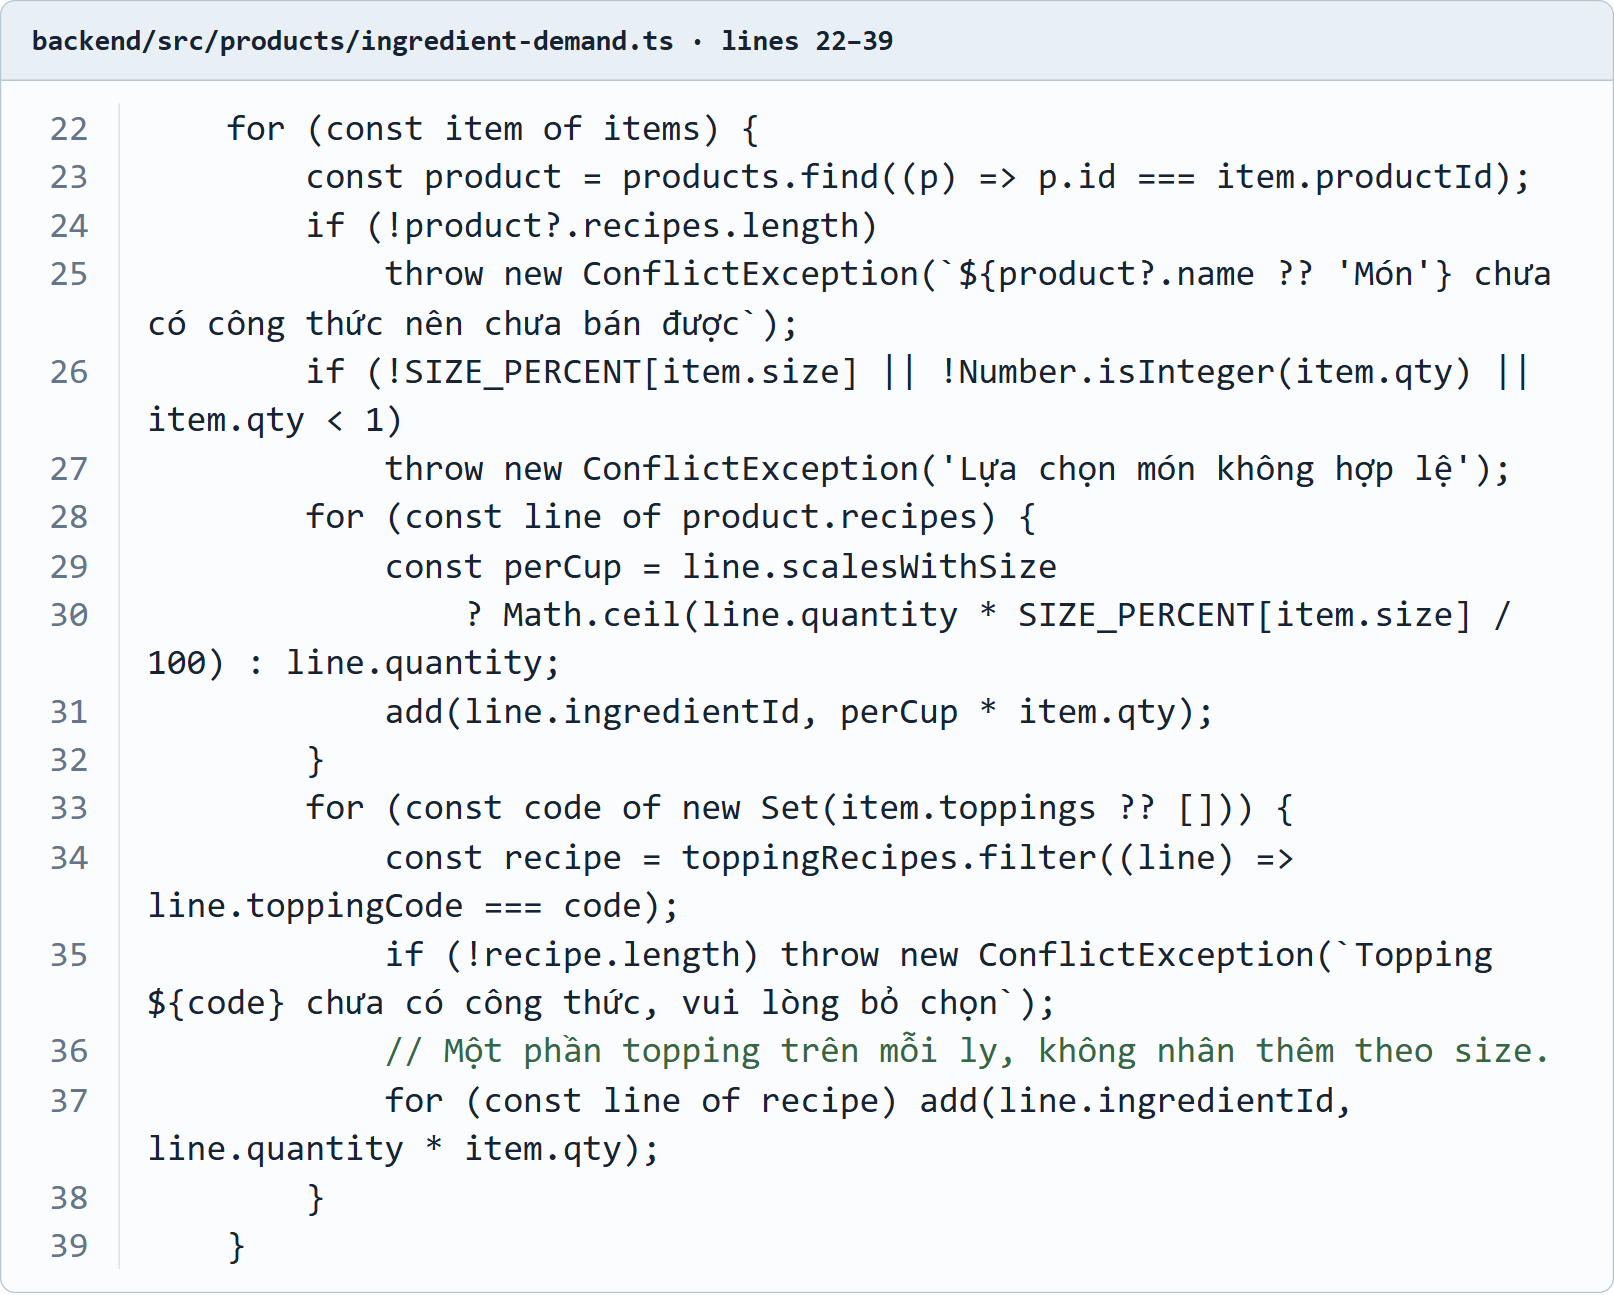
\includegraphics[width=\linewidth,height=.79\textheight,keepaspectratio]{assets/inventory/code-demand.png}
\caption{ingredientDemand: tính size, vật tư cố định, topping và cộng gộp nguyên liệu}
\end{figure}
\clearpage
\begin{figure}[p]\centering
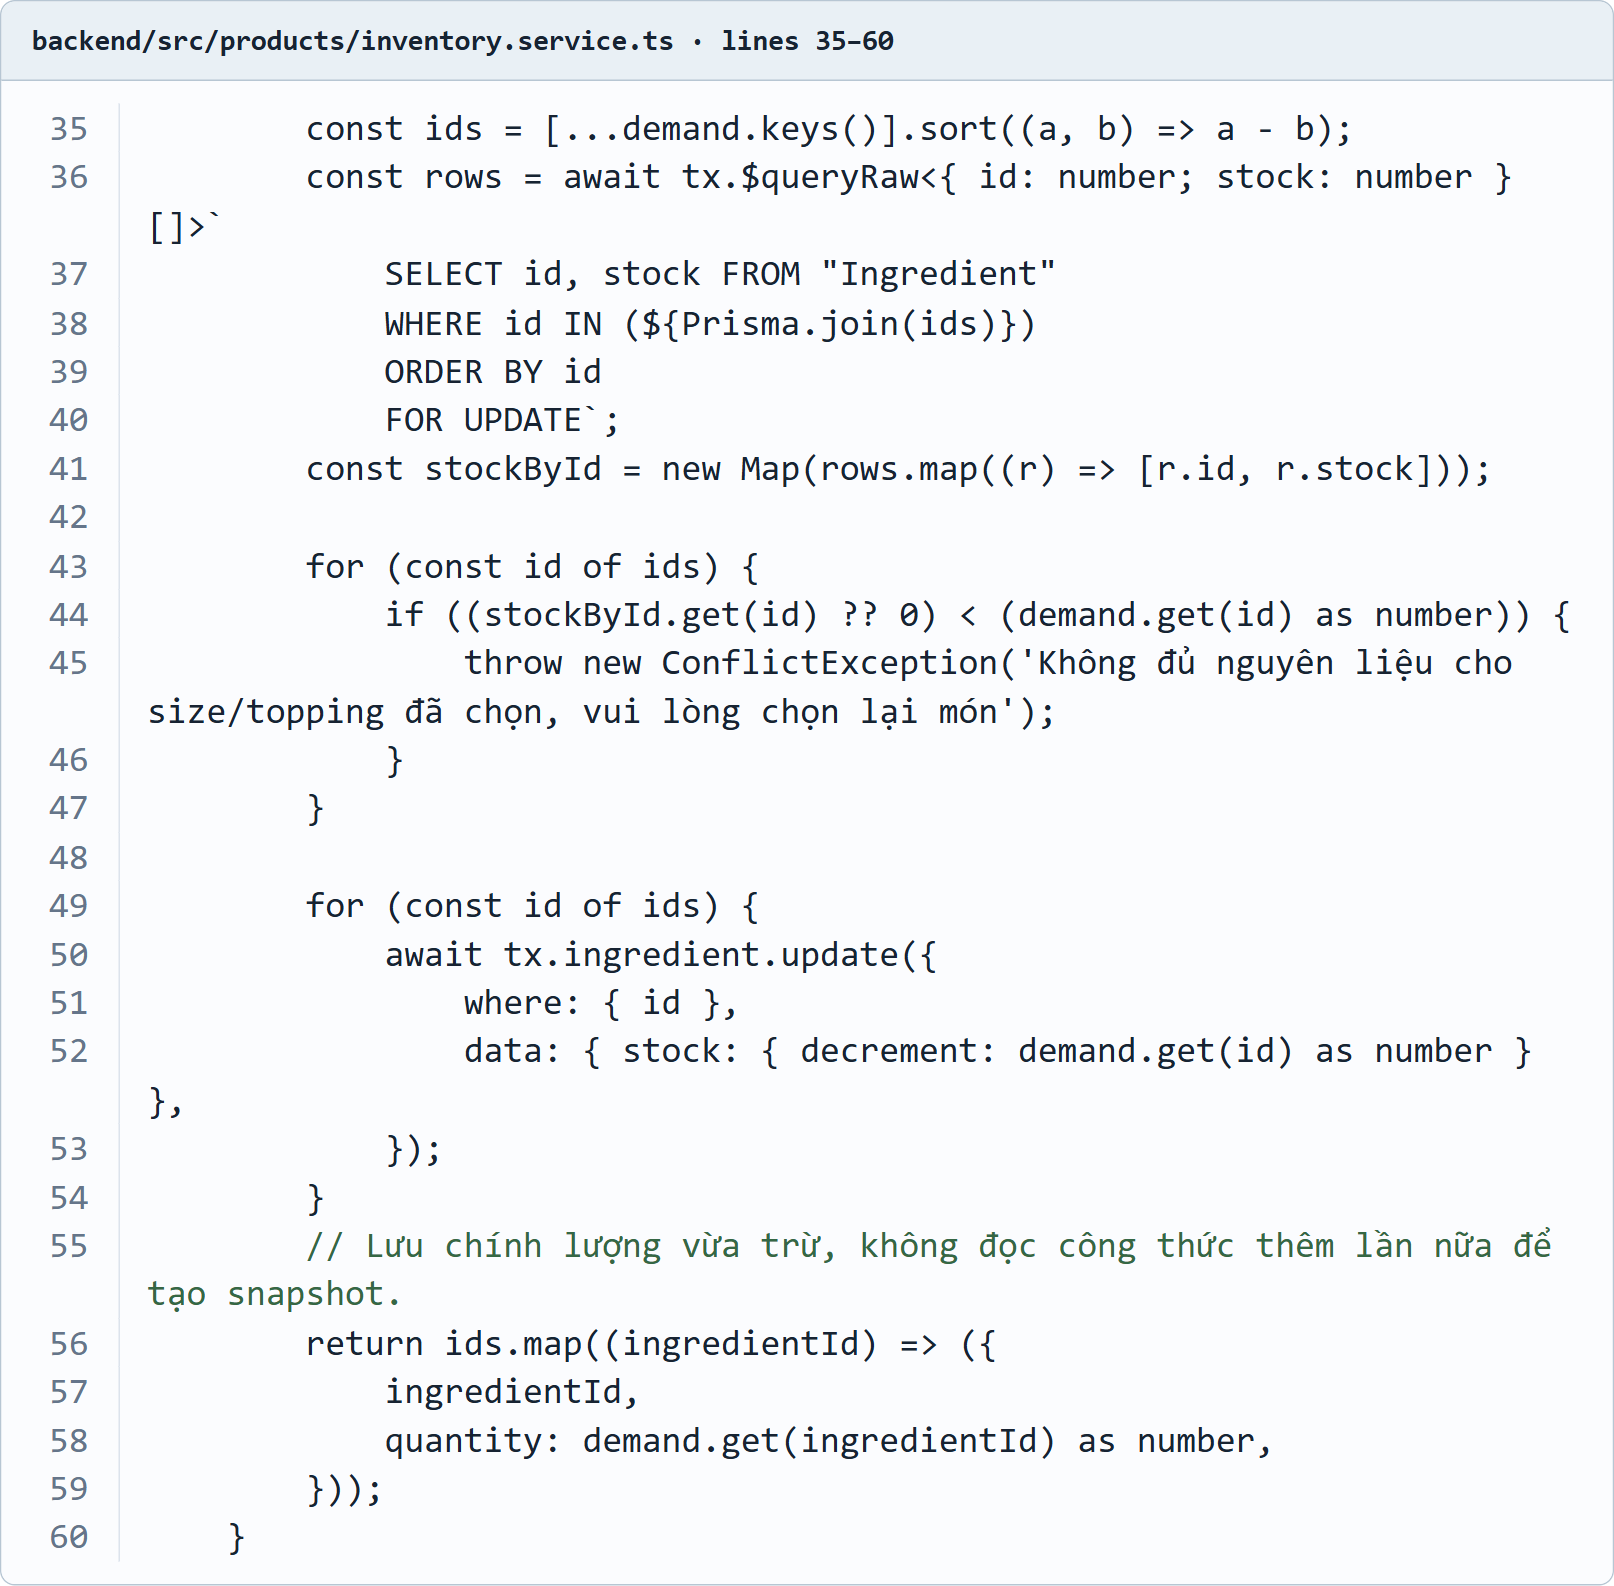
\includegraphics[width=\linewidth,height=.79\textheight,keepaspectratio]{assets/inventory/code-reserve.png}
\caption{reserve: khóa dòng theo thứ tự id, kiểm kho, trừ và trả snapshot}
\end{figure}
\clearpage
\begin{figure}[p]\centering
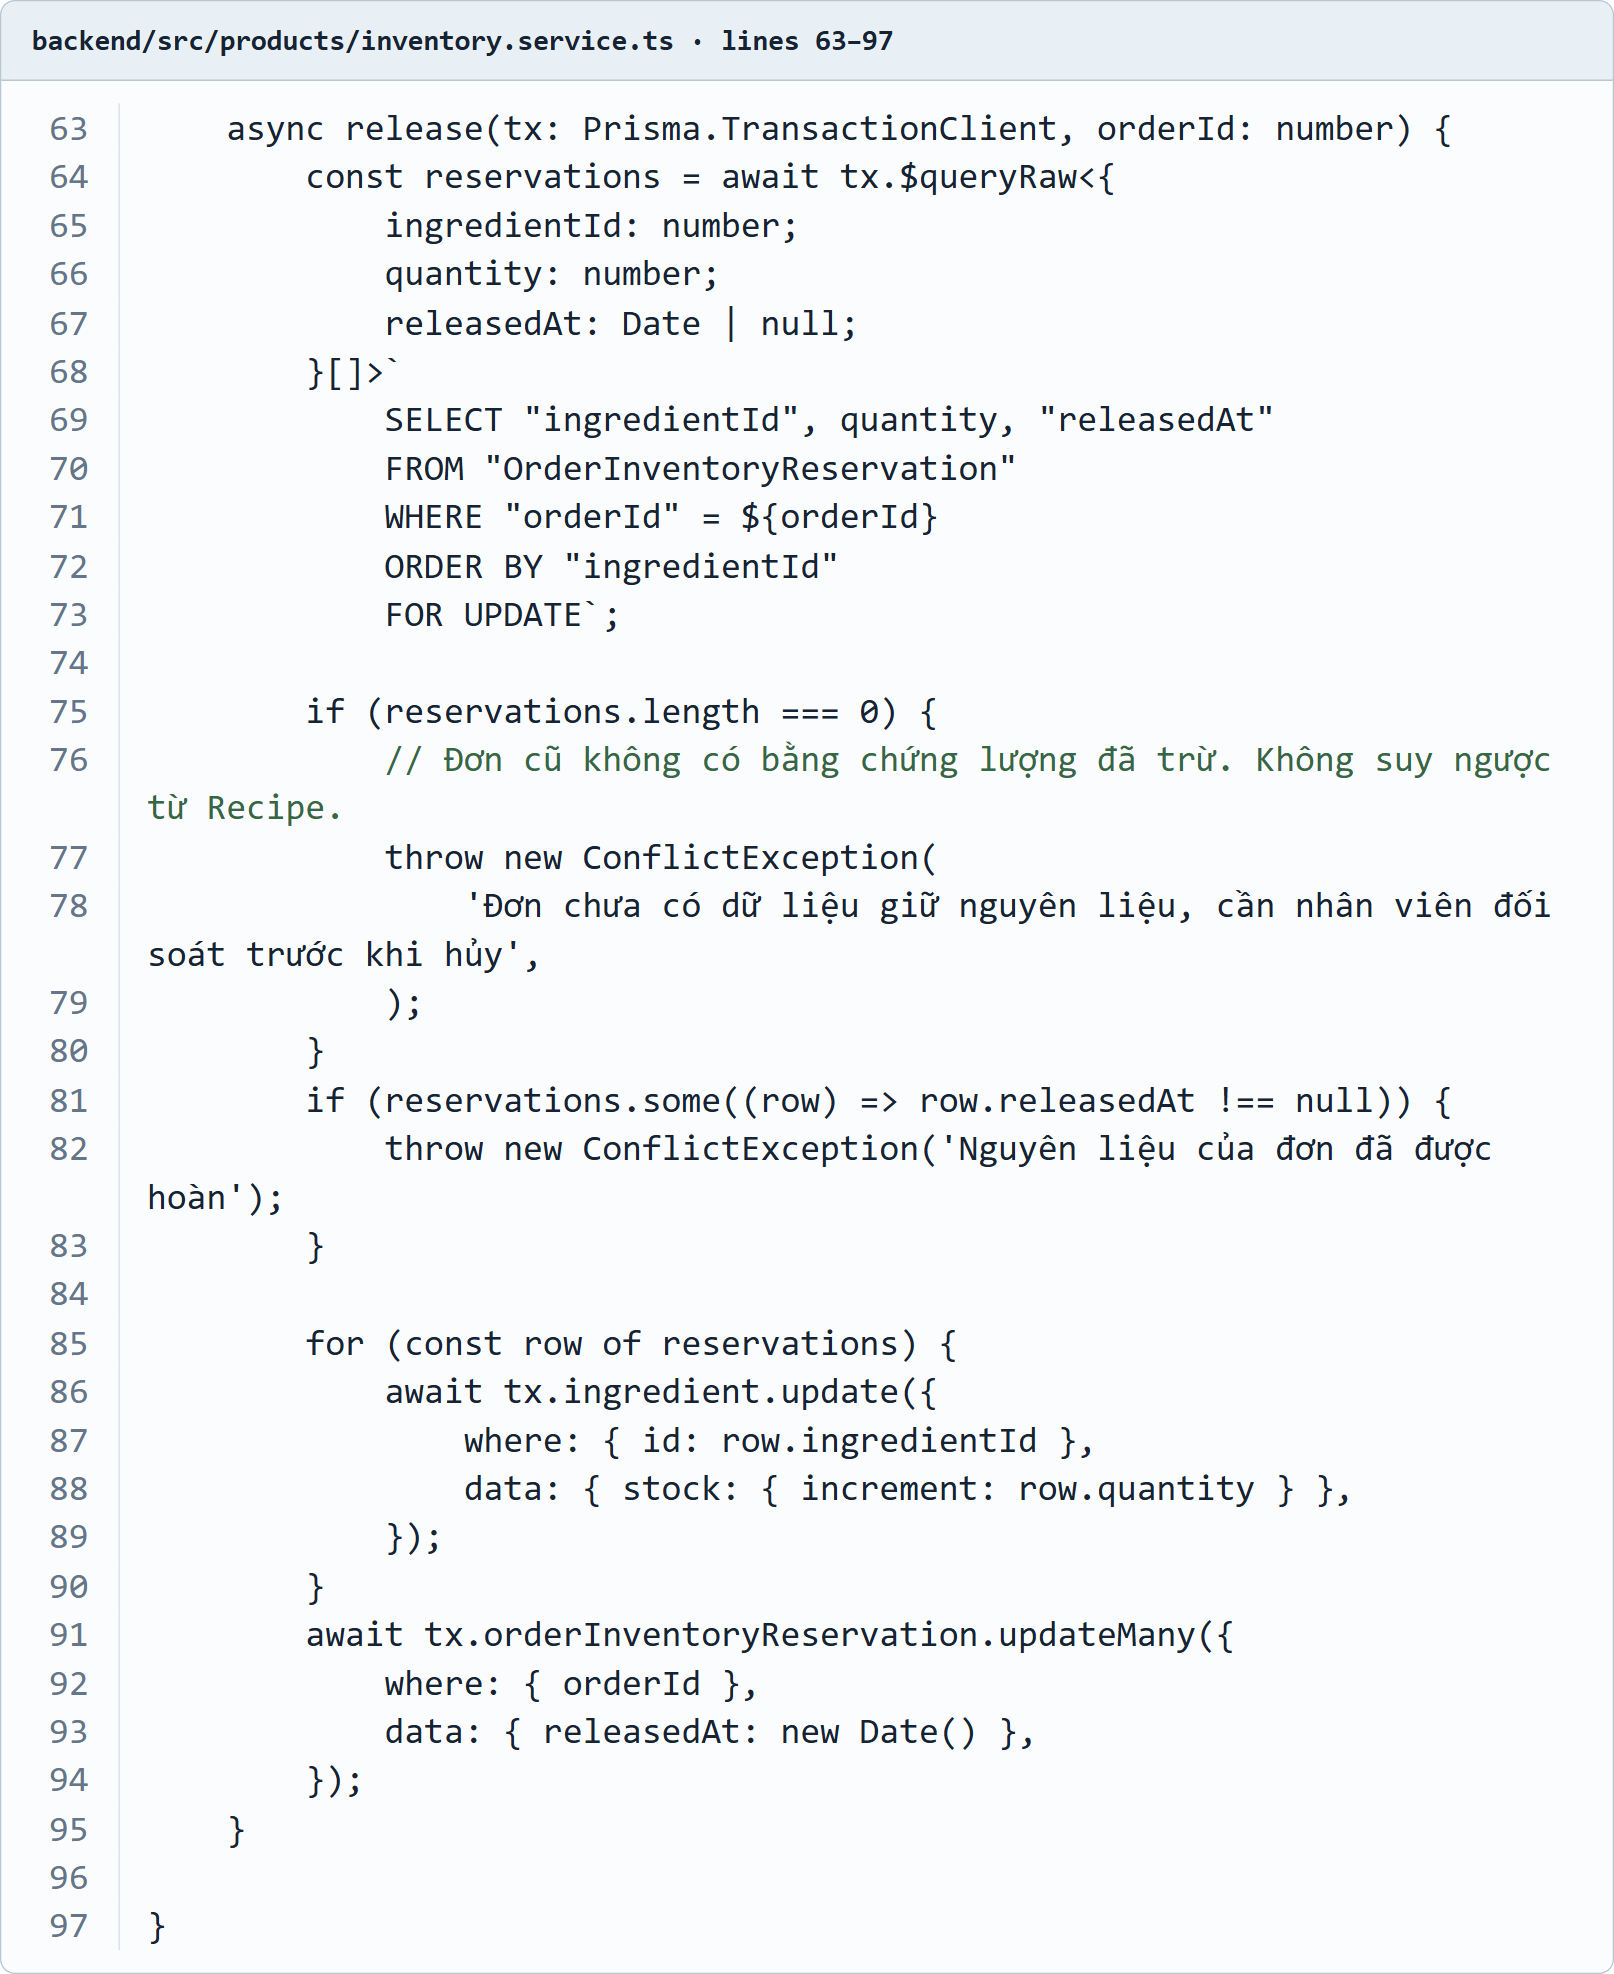
\includegraphics[width=\linewidth,height=.79\textheight,keepaspectratio]{assets/inventory/code-release.png}
\caption{release: khóa snapshot, chặn hoàn lại và cộng đúng lượng lịch sử}
\end{figure}
\clearpage
\begin{figure}[p]\centering
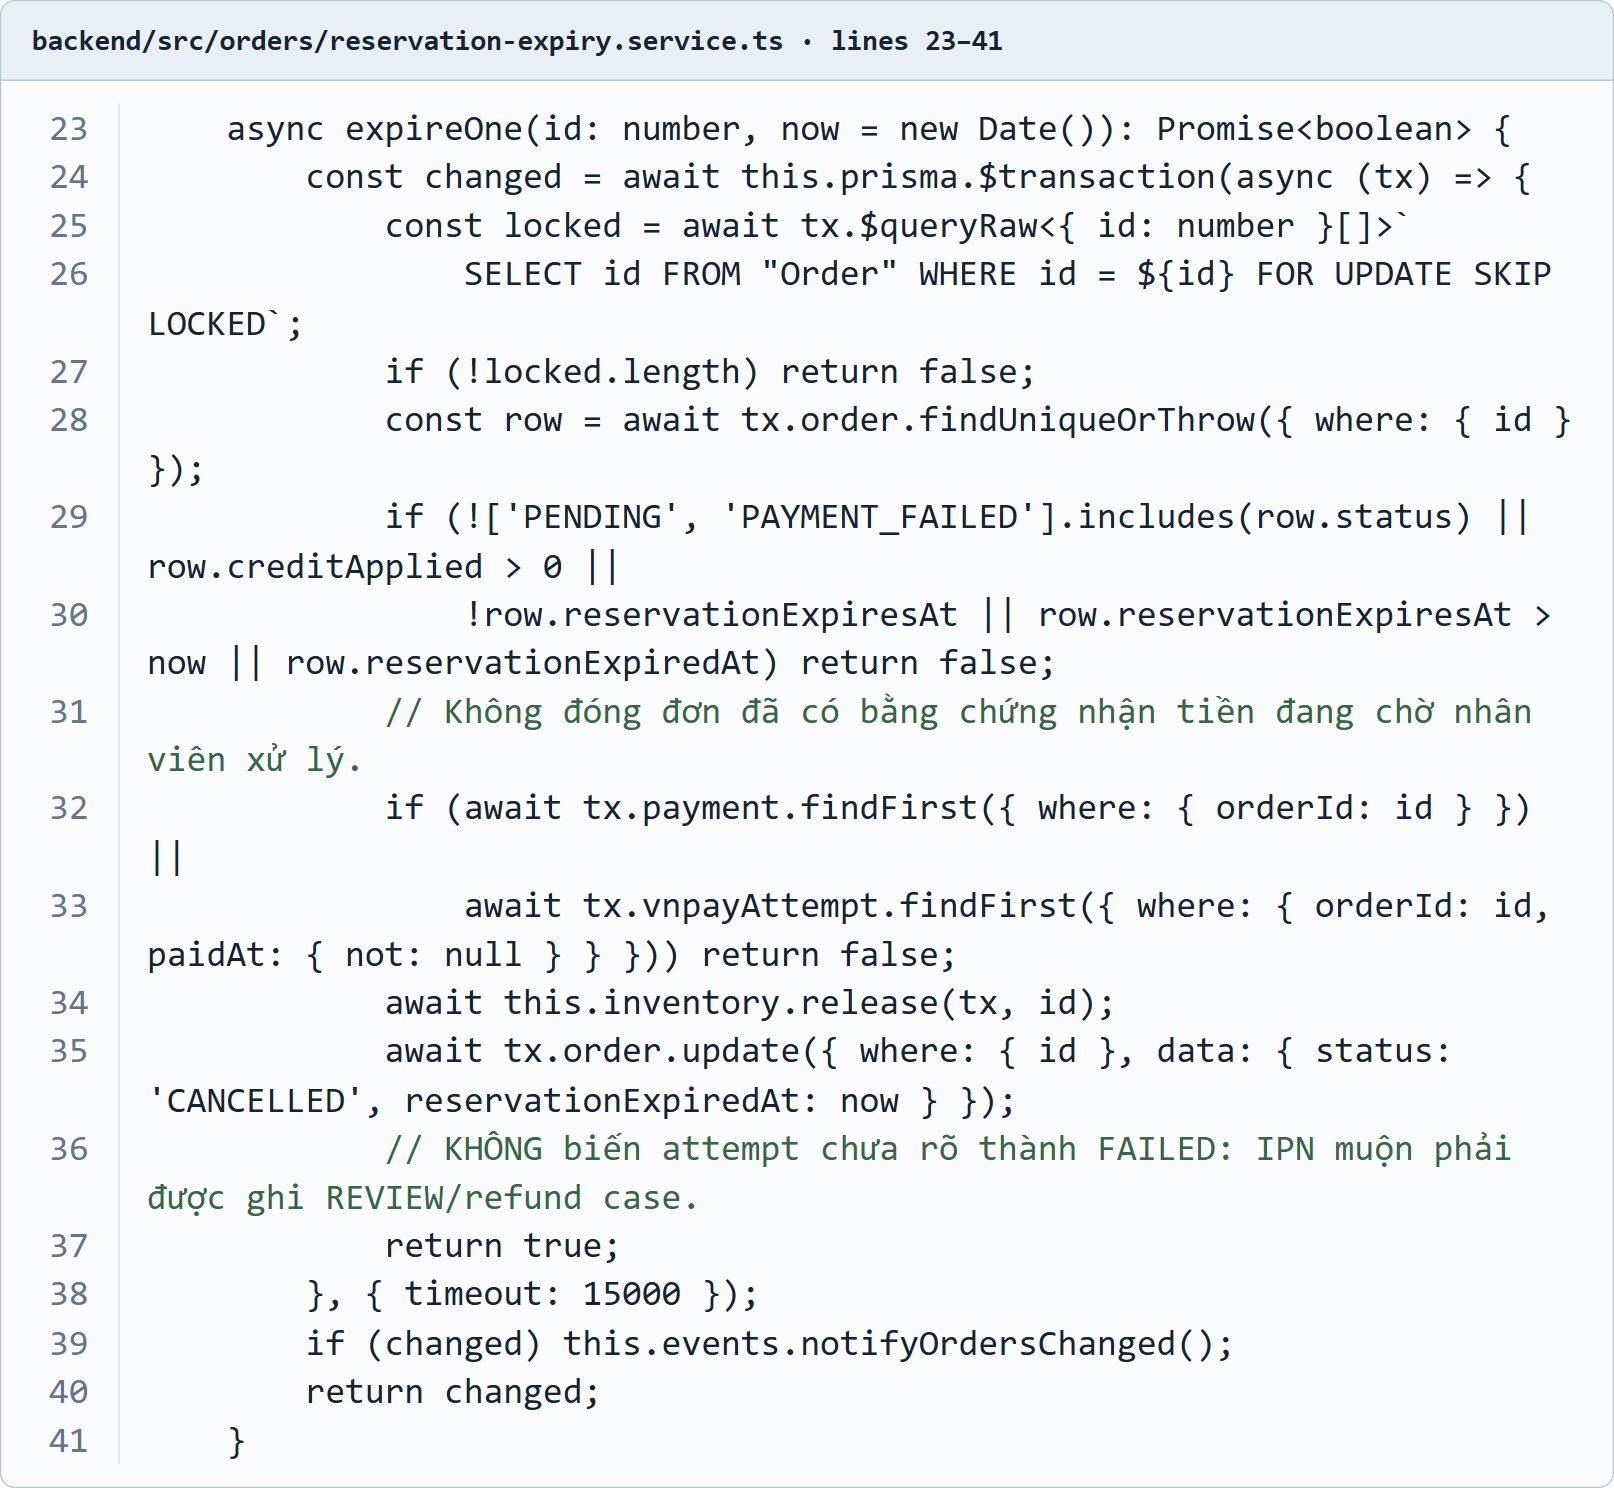
\includegraphics[width=\linewidth,height=.79\textheight,keepaspectratio]{assets/inventory/code-expiry.png}
\caption{expireOne: phối hợp worker, kiểm tra bằng chứng thanh toán và đóng đơn nguyên tử}
\end{figure}
\clearpage


\subsubsection{Khuyến mãi và điểm thưởng}
\label{sec:promotions-implementation}
PromotionsService.findValid dùng được với PrismaService khi xem trước và TransactionClient khi đặt hàng. calcDiscount/calcPoints là hàm thuần, tách quy tắc số học khỏi database để kiểm thử độc lập. OrdersService tạo dòng món theo giá backend, tính subtotal, kiểm voucher rồi lưu total/discount cùng đơn và snapshot kho trong một transaction.

LoyaltyService.award nhận cùng TransactionClient của thanh toán. Khi points dương, UPDATE User dùng increment nguyên tử, lấy số dư mới rồi ghi LoyaltyTransaction EARN. Payment, PAID, số dư và sổ điểm cùng commit hoặc cùng rollback; gửi lại kết quả đã xử lý không được gọi lại để cộng điểm thêm. Unique sổ điểm là lớp bảo vệ bổ sung, không thay thế kiểm settlement dưới khóa Order.

Hai đơn khác nhau cùng trả cho một User dùng phép increment tránh ghi đè số dư đọc cũ. Đổi bằng giá chỉ chuyển credit, không gọi award; đổi cao hơn gọi award qua thanh toán phần chênh lệch. Frontend đọc lại thông tin tài khoản sau kết quả thanh toán để hiển thị điểm do backend trả.

\begin{figure}[htbp]\centering
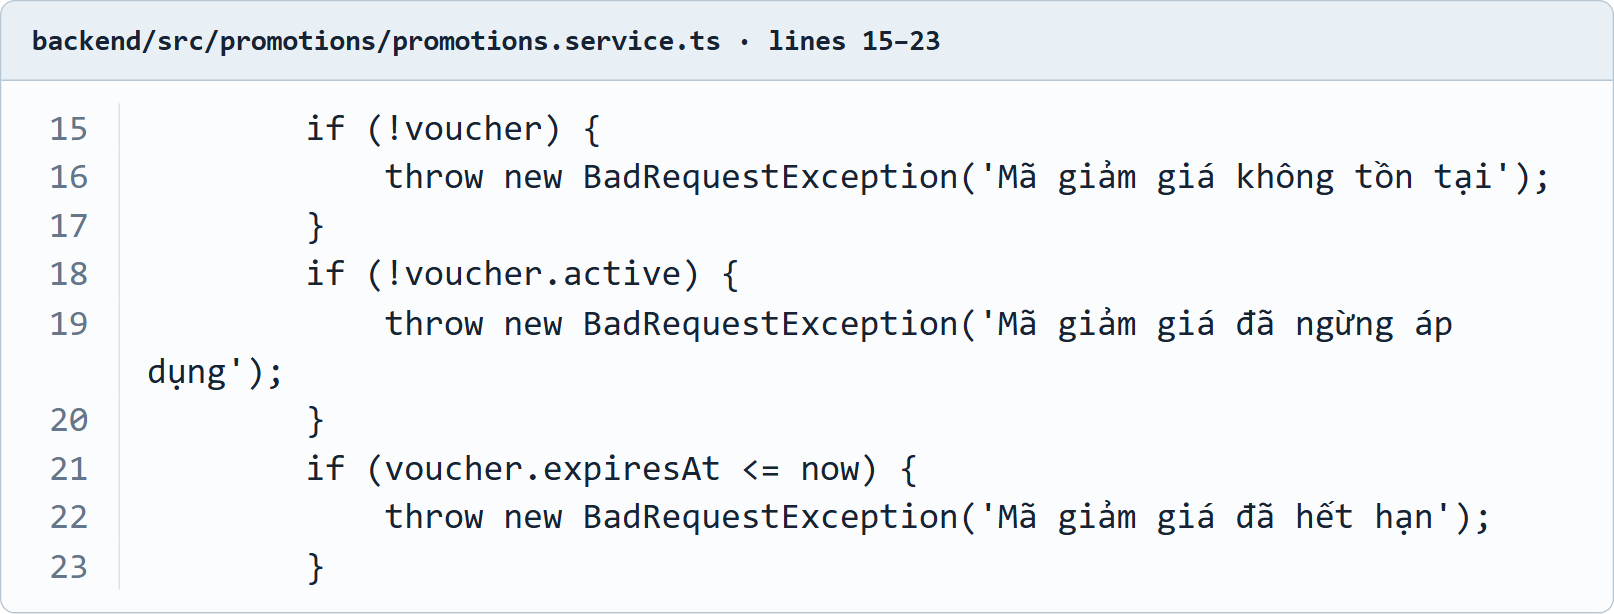
\includegraphics[width=.92\linewidth,height=.24\textheight,keepaspectratio]{assets/promotions/code-validation.png}
\caption{findValid kiểm mã, hiệu lực và hạn trước khi áp dụng}
\vspace{3mm}
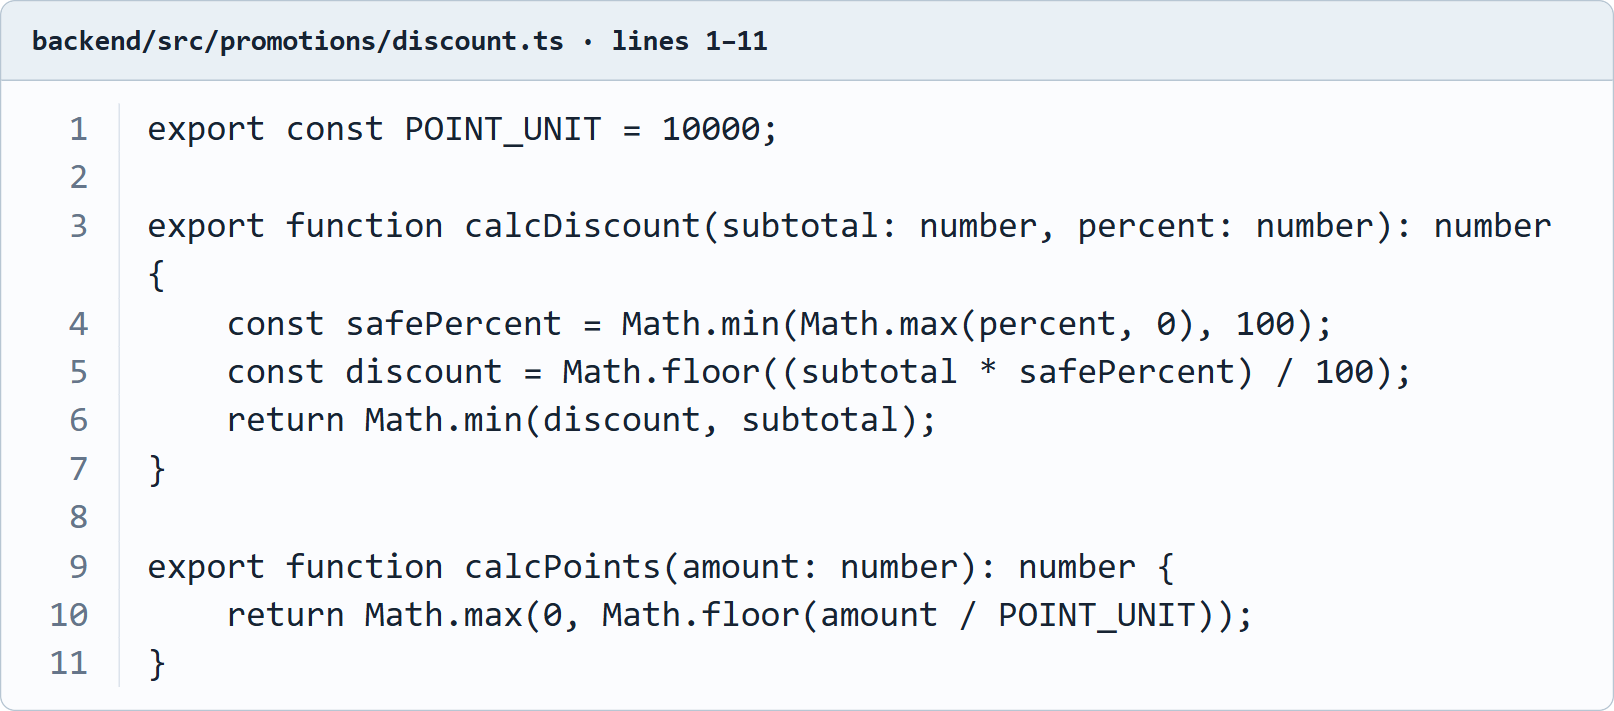
\includegraphics[width=.92\linewidth,height=.18\textheight,keepaspectratio]{assets/promotions/code-calculation.png}
\caption{Hai hàm thuần tính tiền giảm và điểm với quy tắc làm tròn}
\vspace{3mm}
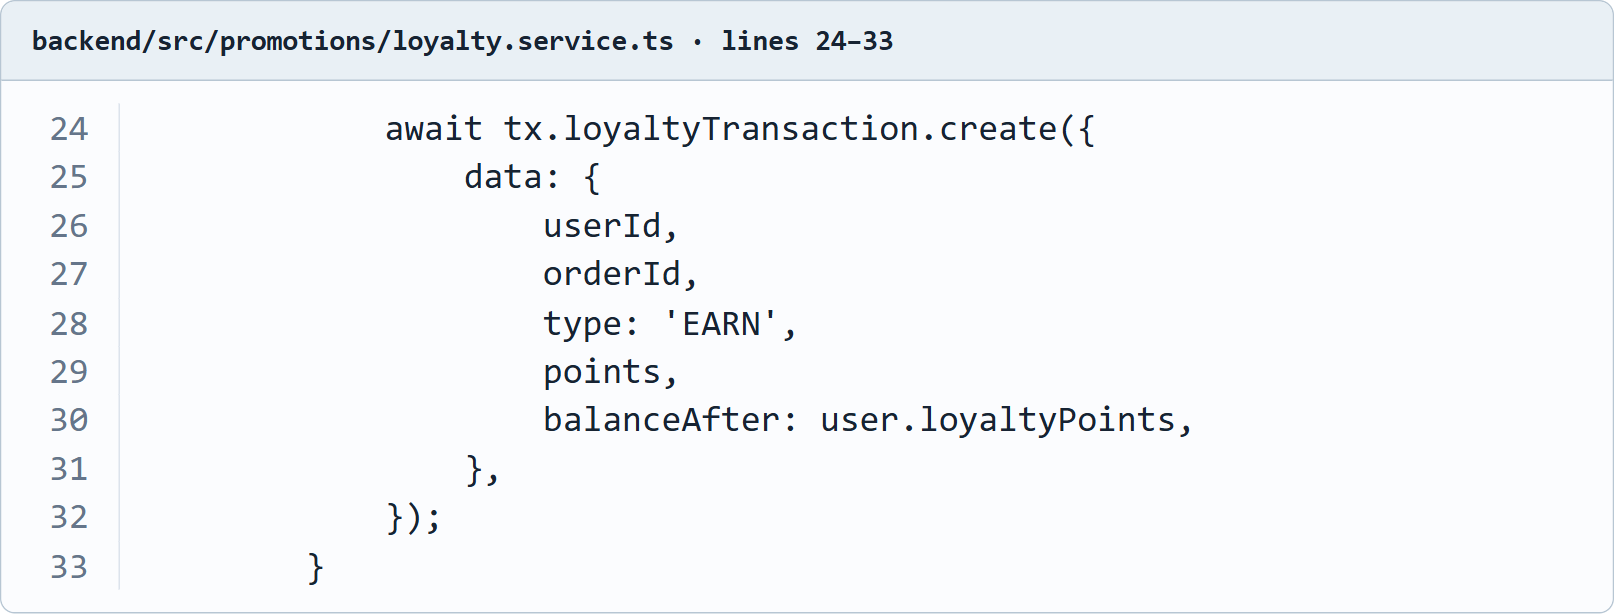
\includegraphics[width=.92\linewidth,height=.27\textheight,keepaspectratio]{assets/promotions/code-ledger.png}
\caption{award ghi EARN cùng số dư sau cập nhật trong transaction thanh toán}
\end{figure}


\subsection{Hiện thực đổi món sau thanh toán}
\label{sec:exchange-implementation}
ExchangeService.quote/quoteIn tính báo giá từ dữ liệu backend; request kiểm quyền, trạng thái, yêu cầu chờ và key trước khi lưu báo giá. withdraw rút yêu cầu bằng trạng thái/version. decide thực hiện quyết định của quầy. Hàng đợi hỗ trợ lọc trạng thái, tìm kiếm và phân trang; frontend ExchangeWorkspace giữ giỏ đổi riêng, không trộn với lần mua thông thường.

\subsubsection{Một quyết định, một transaction}
decide khóa Order nguồn trước, đọc lại OrderExchange và kiểm version/REQUESTED. Khi duyệt, kiểm nguồn còn PAID và tiền đã áp dụng khớp; dùng quotedLines để giữ thành tiền đã chấp nhận. Tiếp theo khóa tập hợp nguyên liệu cũ và mới theo id tăng dần, hoàn snapshot cũ, reserve lựa chọn mới theo size/topping, tạo Order thay thế và snapshot, chuyển credit rồi đóng Order nguồn. Cuối cùng cập nhật quyết định, tăng version và commit. Thiếu nguyên liệu mới hoặc lỗi bất kỳ làm rollback cả bước hoàn cũ.

\subsubsection{Tranh chấp với pha chế và thao tác quầy}
Luồng bắt đầu pha và quyết định đổi cùng khóa Order. API bắt đầu pha kiểm yêu cầu REQUESTED; API duyệt kiểm nguồn PAID. Vì vậy thao tác dựa trên trạng thái cũ bị chặn sau khi trạng thái đã thay đổi. UPDATE yêu cầu có điều kiện id/version/status và kiểm count=1 bảo vệ trước thao tác đã cũ; version tăng sau khi duyệt, từ chối hoặc rút. Thông báo UI phát sau commit.

\subsubsection{Bảo toàn tiền đã chuyển}
Đơn thay thế có credit không đi qua tự hủy/hết hạn thông thường của đơn chưa từng trả tiền. Các thao tác giữ/hoàn tài nguyên tái sử dụng cơ chế mục~\ref{sec:inventory-implementation}; thu chênh lệch tái sử dụng VNPay mục~\ref{sec:vnpay-implementation}. Không cộng credit thành một Payment mới, vì việc đó sẽ làm sai thống kê dòng tiền và có thể cộng điểm trùng.

\begin{figure}[htbp]\centering
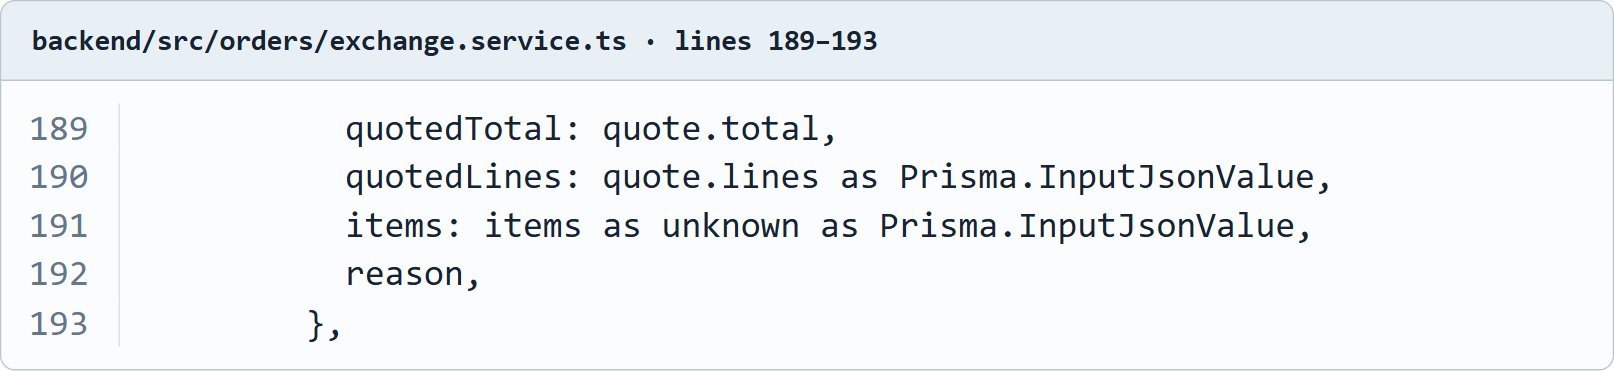
\includegraphics[width=.94\linewidth,height=.25\textheight,keepaspectratio]{assets/exchange/code-quote.png}
\caption{request lưu báo giá và nội dung đã được khách xác nhận}
\vspace{3mm}
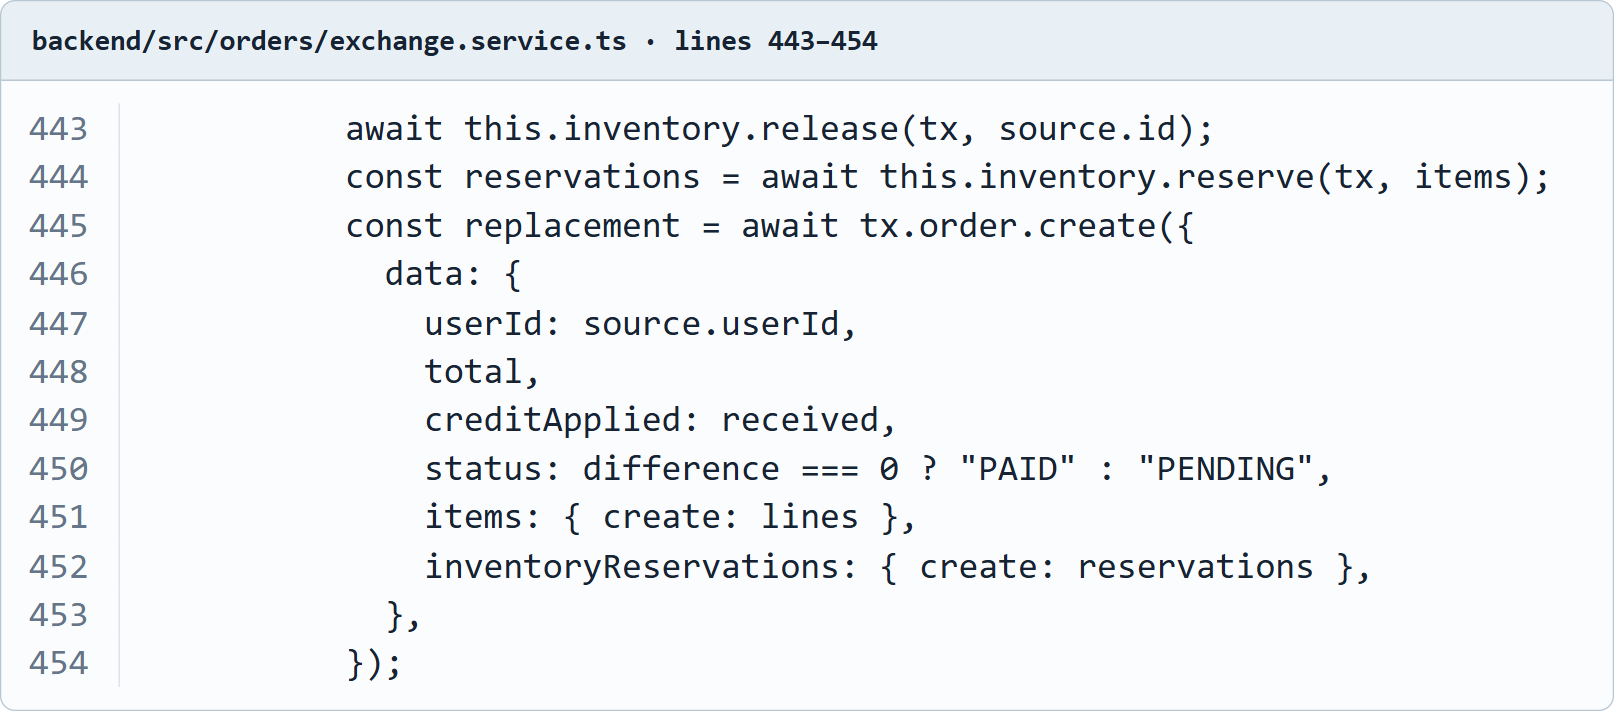
\includegraphics[width=.94\linewidth,height=.26\textheight,keepaspectratio]{assets/exchange/code-replacement.png}
\caption{Hoàn snapshot cũ, giữ lựa chọn mới và tạo đơn chuyển credit trong transaction}
\vspace{3mm}
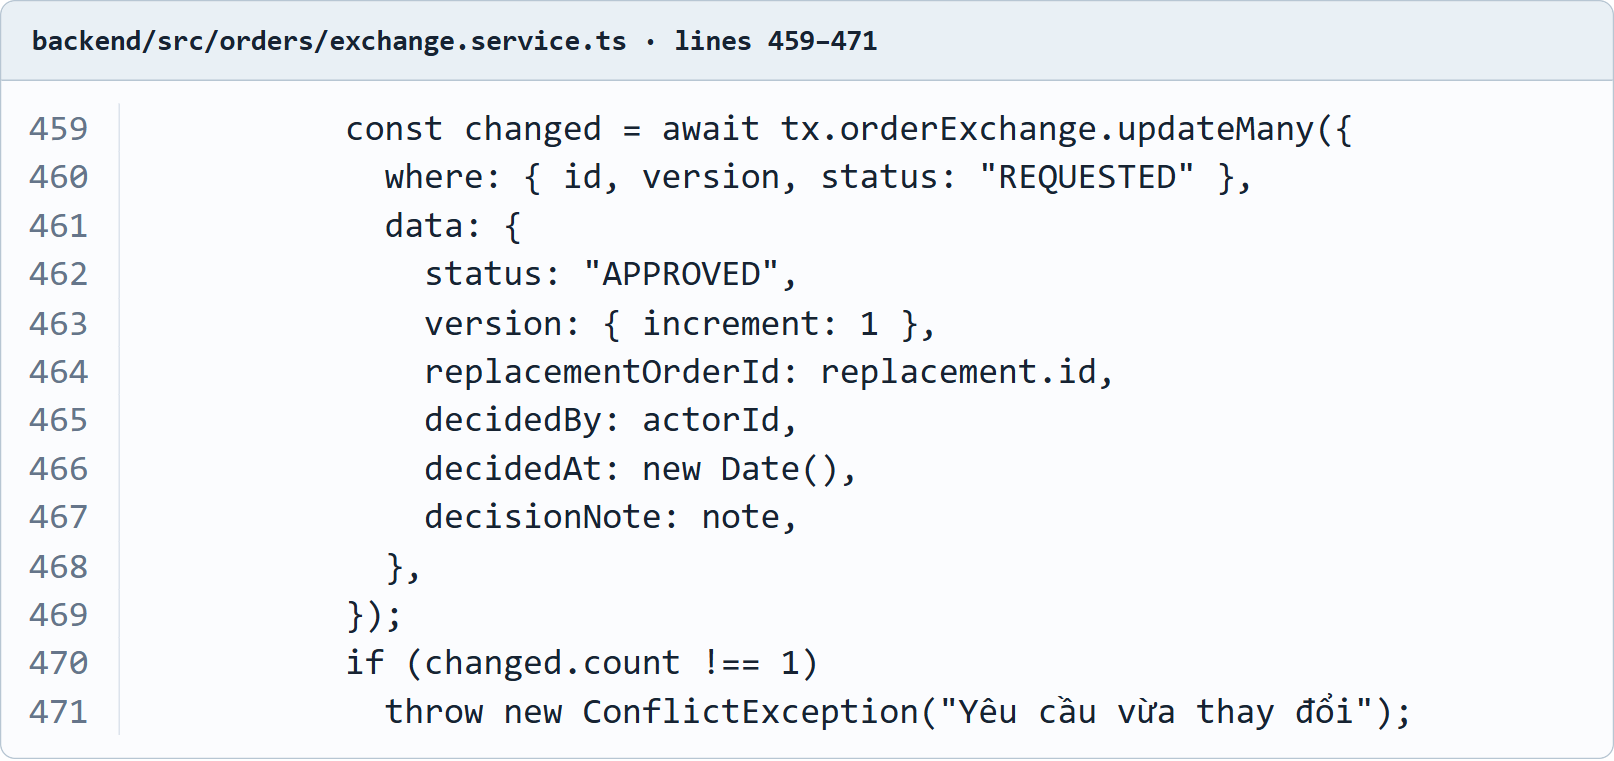
\includegraphics[width=.94\linewidth,height=.25\textheight,keepaspectratio]{assets/exchange/code-version.png}
\caption{Quyết định cập nhật có điều kiện theo version và trạng thái REQUESTED}
\end{figure}


\subsection{Hiện thực quầy và cập nhật theo thời gian thực}
\label{sec:staff-implementation}
\subsubsection{Kiểm soát chuyển trạng thái tại backend}
StaffOrdersController nhận PATCH trạng thái qua JwtAuthGuard/RolesGuard; DTO chỉ nhận PREPARING, READY hoặc COMPLETED. OrdersService.updateStaffStatus khóa Order, đọc lại trạng thái, kiểm yêu cầu đổi chờ và gọi assertTransition. UPDATE kèm điều kiện trạng thái hiện tại, kiểm count trước khi commit. Hai request cùng duyệt một đơn PAID sang PREPARING chỉ có một request hợp lệ; request tiếp theo không được coi PREPARING sang PREPARING là bước mới.

Máy trạng thái là luật chuyển tiếp dùng chung, còn quyền và điều kiện cụ thể nằm ở service. Có cạnh PAID sang CANCELLED không có nghĩa API quầy được hủy tùy ý: luồng đổi món/hủy/hết hạn có kiểm tra riêng. Các phần xử lý tài chính và kho được tham chiếu ở những mục tương ứng, không thực hiện lại khi bấm ``Pha xong'' hoặc ``Đã giao khách''.

\subsubsection{Thông báo sau commit và tải lại dữ liệu}
OrdersGateway dùng namespace /orders-live, phát orders.changed không payload. notifyOrdersChanged được gọi sau transaction thành công; rollback hoặc replay không làm một kết quả chưa commit xuất hiện như thành công trên màn hình khác.

Hook useOrdersLive đăng ký connect/disconnect/connect\_error và orders.changed. Khi kết nối hoặc nhận sự kiện, client tải lại API. Có polling HTTP 15 giây khi tab hiển thị và nút tải lại để hỗ trợ khi mất kênh tức thời. Mỗi refresh hủy request trước bằng AbortController; cleanup gỡ listener, ngắt socket và dọn interval khi component rời màn hình. Thanh trạng thái kết nối chỉ biểu diễn kênh cập nhật, không chứng minh một đơn đã trả tiền hoặc đã pha.

\begin{figure}[htbp]\centering
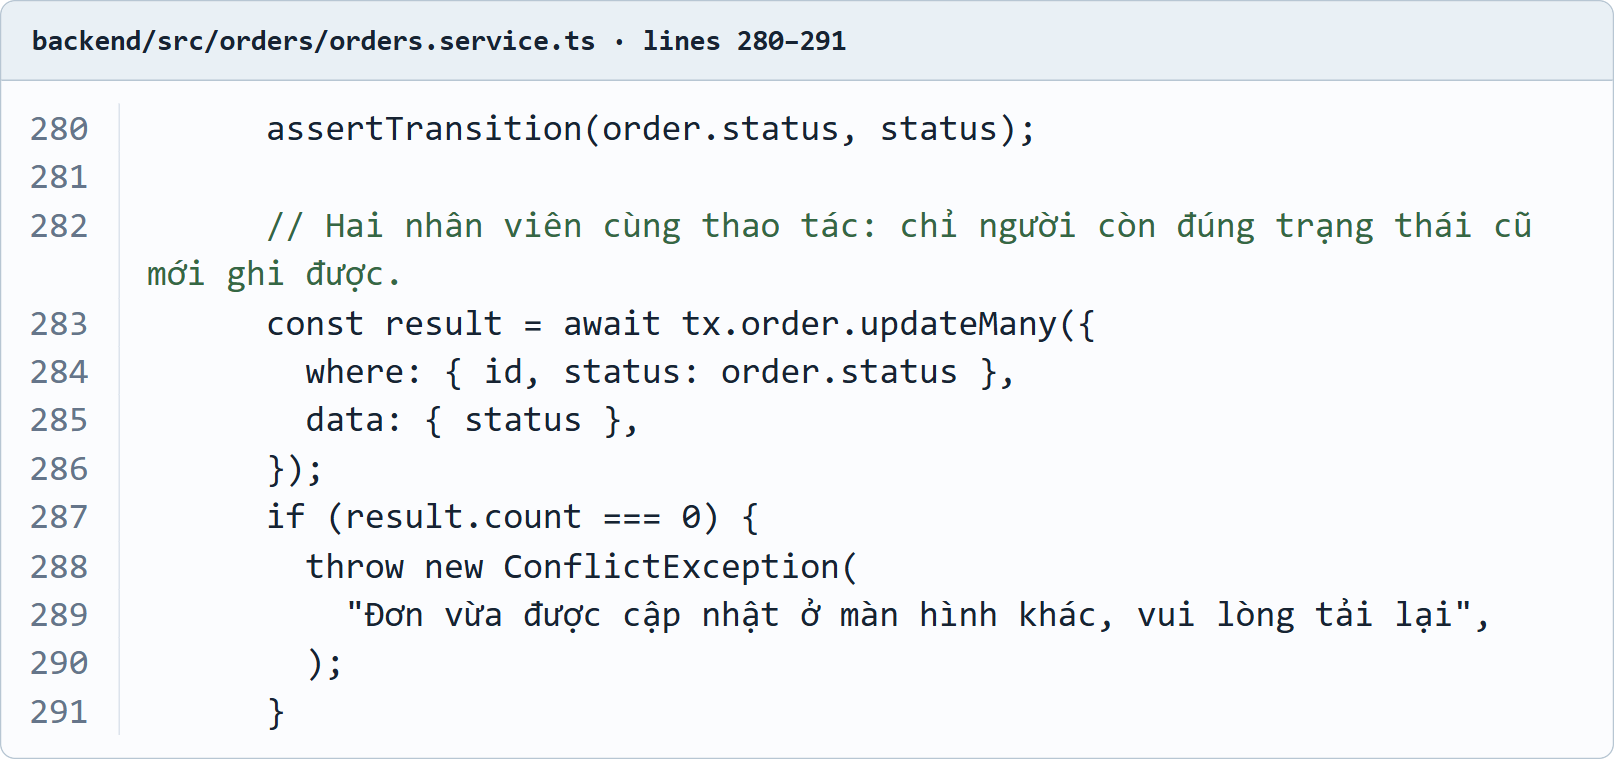
\includegraphics[width=.94\linewidth,height=.25\textheight,keepaspectratio]{assets/staff/code-transition.png}
\caption{Cập nhật có điều kiện sau khi kiểm luật chuyển tiếp và khóa Order}
\vspace{3mm}
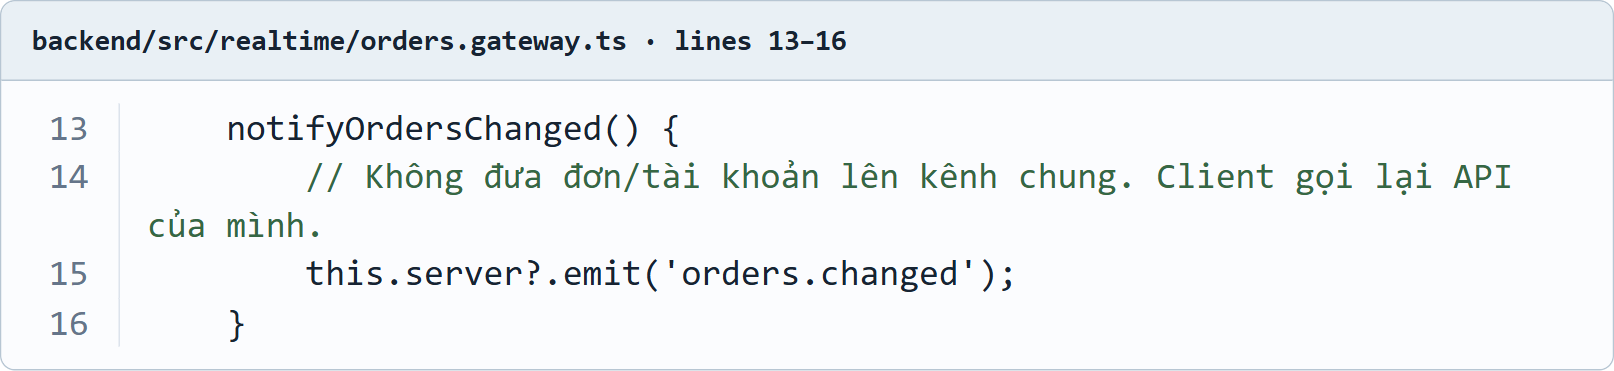
\includegraphics[width=.94\linewidth,height=.16\textheight,keepaspectratio]{assets/staff/code-event.png}
\caption{Gateway chỉ phát tín hiệu thay đổi, không đưa dữ liệu đơn lên kênh chung}
\vspace{3mm}
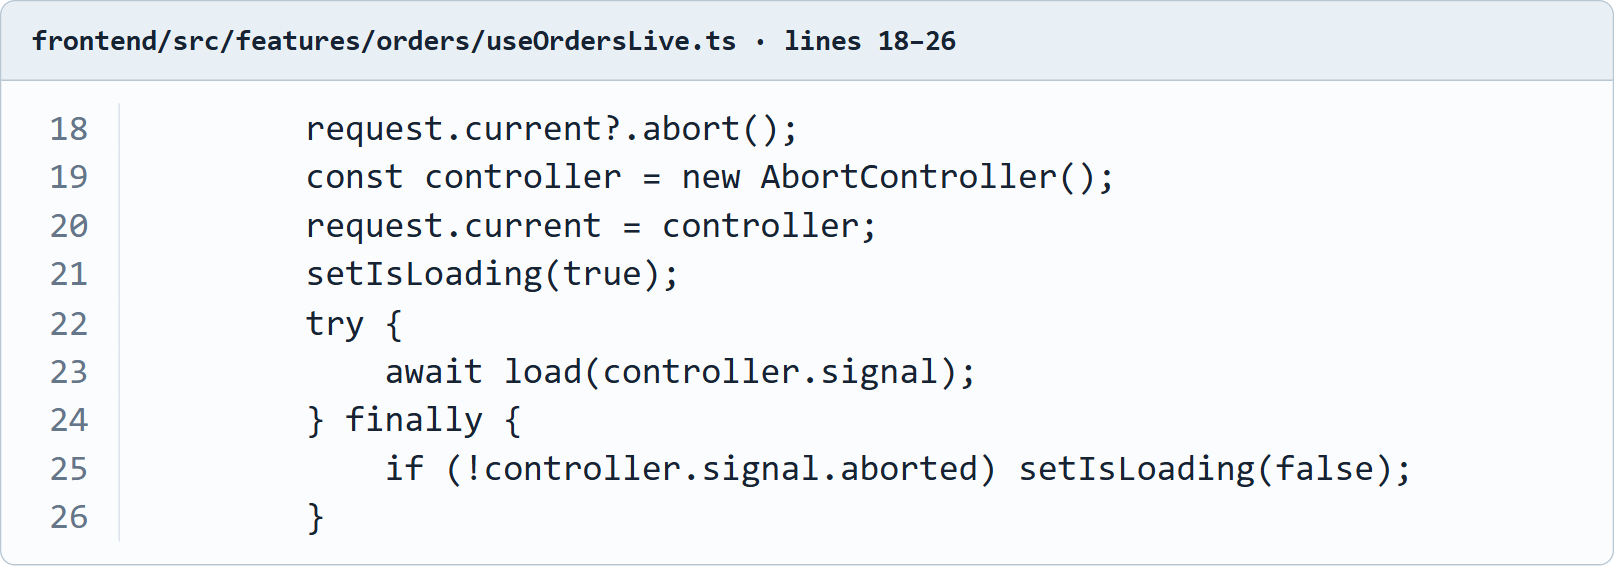
\includegraphics[width=.94\linewidth,height=.25\textheight,keepaspectratio]{assets/staff/code-refresh.png}
\caption{Client chỉ giữ request tải mới và hủy request cũ khi refresh}
\end{figure}


\subsection{Đóng gói và triển khai}
Trong môi trường phát triển, PostgreSQL chạy qua Docker Compose; backend và frontend chạy ở hai terminal riêng. Việc đóng gói dịch vụ gắn với cấu hình mạng, biến môi trường và kiểm tra trạng thái sẵn sàng. Seed chạy chủ động cho dữ liệu mẫu; migration áp dụng có kiểm soát để bảo toàn dữ liệu.

\newpage
%%%%%%%%%%%%%%%%%%%%%%%%%%%%%%%%%
\section{Kiểm thử và kết quả}
\subsection{Chiến lược kiểm thử}
Nhóm dùng hai loại kiểm thử tự động bằng Vitest:
\begin{itemize}
	\item \textbf{Test đơn vị} (\texttt{npm run test}): kiểm tra các hàm thuần như state machine và tính giảm giá, chạy trong vài giây và không cần cơ sở dữ liệu.
	\item \textbf{Test tích hợp API} (\texttt{npm run test:e2e}): dựng cả ứng dụng NestJS và gọi API thật bằng Supertest trên PostgreSQL thật. Mỗi test tự tạo người dùng, sản phẩm và đơn tạm rồi xóa đi sau khi chạy, không đụng vào dữ liệu mẫu.
\end{itemize}
Test API tập trung vào hợp đồng và dữ liệu; browser E2E kiểm tra thao tác xuyên suốt từ trình duyệt tới backend và database. Dùng cơ sở dữ liệu kiểm thử riêng. Các lệnh test chạy trong thư mục \texttt{backend}, và test end-to-end cần cơ sở dữ liệu đang chạy.

\subsection{Kiểm thử các quy tắc toàn vẹn nghiệp vụ}
\begin{table}[h!]
\centering
\footnotesize
\begin{tabularx}{\textwidth}{|p{0.22\linewidth}|p{0.28\linewidth}|X|}
\hline
\textbf{Yêu cầu} & \textbf{Tệp test} & \textbf{Nội dung kiểm tra} \\ \hline
(a) Chặn chuyển trạng thái sai & \path{order-state-machine.spec.ts} và các ca hủy đơn trong \path{payments.e2e-spec.ts} & Các bước nhảy cóc như PENDING sang READY bị chặn; COMPLETED và CANCELLED không đi tiếp; hủy đơn hai lần và thanh toán đơn đã hủy bị từ chối \\ \hline
(b) Gửi 2 lần cùng \texttt{Idempotency-Key} chỉ tạo 1 đơn & \path{order-idempotency.e2e-spec.ts} và \path{payments.e2e-spec.ts} & Gửi liên tiếp và gửi đồng thời cùng khóa chỉ tạo một Order ở test tạo đơn; test thanh toán chỉ tạo 1 dòng Payment và cùng một \texttt{paymentId} \\ \hline
(c) Đặt đồng thời không vượt tồn kho & \path{inventory.e2e-spec.ts} & 10 đơn đồng thời cho món còn 3 phần thì đúng 3 đơn thành công, 7 đơn bị từ chối, kho về 0 \\ \hline
Khuyến mãi và điểm thưởng & \path{discount.spec.ts}, \path{promotions.e2e-spec.ts} & Tính giảm giá và điểm đúng; mã sai, hết hạn hoặc đã tắt bị từ chối; điểm chỉ cộng một lần \\ \hline
\end{tabularx}
\caption{Ánh xạ giữa quy tắc nghiệp vụ và các test}
\end{table}

\subsection{Danh sách test case tự động}
\begin{longtable}{|p{0.30\linewidth}|p{0.60\linewidth}|}
\hline
\textbf{Tệp test} & \textbf{Các ca kiểm tra chính} \\ \hline
\endhead
\path{order-state-machine.spec.ts} & Luồng thành công PENDING, PAID, PREPARING, READY, COMPLETED; thanh toán lỗi rồi thử lại; 9 ca chuyển trạng thái sai bị chặn; hai trạng thái cuối không đi tiếp; danh sách chuyển tiếp hợp lệ khớp đúng bảng luật \\ \hline
\path{discount.spec.ts} & Giảm 10\% của 120.000đ là 12.000đ; làm tròn xuống; không giảm quá tổng tiền; phần trăm không dương thì không giảm; dưới 10.000đ chưa được điểm; 108.000đ được 10 điểm \\ \hline
\path{payments.e2e-spec.ts} & Gửi hai lần liên tiếp và đồng thời cùng khóa; cùng khóa cho đơn khác bị 409; thanh toán lỗi rồi thử lại; thanh toán lại đơn PAID bị 409; thiếu header bị 400; hủy đơn hai lần và đơn đã thanh toán không hủy được \\ \hline
\path{inventory.e2e-spec.ts} & 10 đơn đồng thời cho món còn 3 phần; 6 đơn số lượng 2 cho món còn 5 phần; đơn lớn hơn tồn kho bị từ chối; hai dòng cùng món được cộng dồn; đơn nhiều dòng thiếu một món bị hoàn tác toàn bộ; hủy đơn hoàn kho đúng một lần \\ \hline
\path{promotions.e2e-spec.ts} & Mã hợp lệ không phân biệt hoa thường; mã không tồn tại, hết hạn, đã tắt bị 400; đơn có mã giảm đúng 10\%; mã sai thì không tạo đơn và không trừ kho; thanh toán đúng số tiền sau giảm và cộng điểm đúng một lần \\ \hline
\caption{Các test tự động} \\
\end{longtable}

\subsection{Kiểm chứng luồng đặt hàng, giữ kho và hoàn kho}
\label{sec:inventory-tests}
Kiểm thử tách thành ba lớp: hàm tính định lượng thuần; API tích hợp với PostgreSQL để kiểm tra transaction/khóa/ràng buộc; giao diện để kiểm tra lựa chọn, thông báo và điều hướng. Dữ liệu thử được tạo riêng để kết quả có thể kiểm tra trực tiếp từ tồn kho, snapshot và trạng thái đơn.

\begingroup\small
\begin{longtable}{|p{.10\linewidth}|p{.43\linewidth}|p{.36\linewidth}|}
\hline\textbf{Ca} & \textbf{Thiết lập và thao tác} & \textbf{Điều kiện kiểm tra}\\\hline\endhead
KHO-01 & Hai ly M, cơ bản 18g, topping dùng chung 5g, một ly nhựa mỗi ly. & Giữ 56g và hai ly; không nhân ly nhựa theo hệ số size.\\\hline
KHO-02 & Topping làm vượt nguyên liệu dù món cơ bản còn đủ. & Backend trả xung đột; Order và kho không đổi. Availability đúng theo tổ hợp.\\\hline
KHO-03 & Mười đơn đồng thời, kho đủ ba phần. & Đúng ba đơn thành công, bảy đơn bị từ chối; kho về 0.\\\hline
KHO-04 & Hai món khác nhau cùng tranh nguyên liệu cuối đủ một ly L. & Chỉ một đơn thành công, không coi mỗi Product có một kho riêng.\\\hline
KHO-05 & Một đơn nhiều dòng có một nguyên liệu thiếu. & Không lưu đơn một phần, không giữ kho của các dòng còn lại.\\\hline
KHO-06 & Gửi đồng thời cùng key khi còn một phần. & Trả cùng một Order, một lần trừ và một bộ snapshot.\\\hline
KHO-07 & Đặt giữ 40g rồi sửa công thức hoặc thay nguyên liệu. & Hủy vẫn hoàn đúng 40g vào nguyên liệu cũ.\\\hline
KHO-08 & Hai yêu cầu hủy đồng thời, sau đó gọi release lại. & Chỉ một lần hoàn; lần sau bị chặn, releasedAt không tạo thêm stock.\\\hline
KHO-09 & Cố ý ném lỗi sau reserve hoặc sau release. & Rollback cả kho, snapshot và trạng thái Order.\\\hline
KHO-10 & Khách khác hủy đơn; đơn PAID dùng API hủy thường. & Bị từ chối, kho và trạng thái không đổi.\\\hline
KHO-11 & Đơn quá hạn, hai worker cùng xử lý. & Một lần đóng/hoàn, có reservationExpiredAt và thông báo đặt lại.\\\hline
KHO-12 & Đã qua deadline nhưng worker chưa chạy; gửi yêu cầu thanh toán. & Không tạo khoản thanh toán mới cho đơn quá hạn.\\\hline
KHO-13 & IPN thành công đến sau deadline, trước hoặc sau worker. & Không PAID/pha chế; REVIEW và một hồ sơ khoản thu dư; kho được bảo toàn.\\\hline
KHO-14 & QR cũ hết hạn nhưng đơn còn thời gian giữ. & Cấp QR mới; expiry QR không vượt deadline Order, không giữ kho lần hai.\\\hline
KHO-15 & Đơn đã trả tiền hoặc đã dùng credit; worker quét. & Không tự đóng như đơn bỏ thanh toán thông thường.\\\hline
\caption{Các ca kiểm chứng và kết quả mong đợi của quản lý nguyên liệu}
\end{longtable}\endgroup

Các test được tổ chức theo trách nhiệm:
\begin{itemize}
\item \path{inventory.e2e-spec.ts}: cạnh tranh tồn kho, đầu vào và hủy đơn.
\item \path{ingredients.e2e-spec.ts}: công thức và nguyên liệu dùng chung.
\item \path{inventory-snapshot.e2e-spec.ts}: công thức thay đổi, hoàn một lần và rollback.
\item \path{order-idempotency.e2e-spec.ts}: gửi lặp và tranh key tạo đơn.
\item \path{size-topping-expiry.e2e-spec.ts}: định lượng lựa chọn, deadline, worker và IPN muộn.
\end{itemize}
Hàm tính định lượng và chính sách deadline/QR có unit test riêng. Các ca ném lỗi chủ động kiểm tra rollback, vì vậy thông báo lỗi trong log phải được đọc cùng assertion và kết quả PASS của test, không chỉ dựa vào màu log.

\subsubsection{Kết quả kiểm chứng theo phạm vi}
Ngày 12/11/2026, bản vá 13 độc lập được dựng trong staging và chạy trên database thử mới, tách khỏi dữ liệu vận hành. Kết quả ghi nhận gồm 42/42 unit test (7 tệp) và 135/135 API integration test (12 tệp). Các con số là tổng bộ hồi quy của bản vá, bao gồm cả thanh toán, quyền và đổi món; không phải 135 ca chỉ riêng tồn kho. TypeScript backend/frontend, build backend và build production frontend đều đạt trong môi trường kiểm chứng đó.

Ở lần kiểm tra source đã ghép, bộ unit test hiện có ghi nhận 31/31 ca đạt. Hai kết quả có phạm vi bộ test khác nhau và được ghi riêng; kết quả của staging không được quy đổi thành kết quả nghiệm thu toàn bộ nhánh tích hợp. Hồ sơ kiểm chứng của bản vá nằm tại \path{proposed-fixes/13-size-topping-reservation/VALIDATION.md}.

Kiểm tra giao diện dùng Edge headless, kích thước desktop 1280$\times$900 và mobile 390$\times$844, với API fixture để cô lập trạng thái màn hình. Kiểm tra gồm thông báo hết hạn trong chi tiết/lịch sử, CTA đặt lại, không có thao tác hủy trên đơn đã đóng, topping không đủ hàng bị khóa và nút thêm giỏ bị vô hiệu khi chọn tổ hợp hết nguyên liệu. Ảnh dưới là minh chứng UI với dữ liệu thử; kiểm thử API PostgreSQL ở trên mới kiểm tra tính đúng của database và transaction.

\begin{figure}[p]\centering
\includegraphics[width=.43\linewidth,height=.76\textheight,keepaspectratio]{../proposed-fixes/13-size-topping-reservation/screenshots/expired-mobile.png}
\caption{Giao diện thông báo hết thời gian giữ món và yêu cầu đặt lại (API fixture)}
\end{figure}


\subsection{Kiểm chứng thanh toán VNPay}
Unit test kiểm HMAC bằng vector RFC 4231, chuẩn hóa khoảng trắng/ký tự đặc biệt, callback sửa tiền/trường trùng, giờ GMT+7 và chữ ký QueryDr. API integration dùng gateway giả lập có chữ ký test cùng PostgreSQL riêng để chủ động tạo callback lặp, trễ và lỗi giữa transaction.

\begin{table}[htbp]\centering\small
\begin{tabularx}{\linewidth}{|p{.13\linewidth}|X|}\hline
\textbf{Mã} & \textbf{Hành vi cần chứng minh}\\\hline
PAY-01 & Backend quyết định amount/merchant; cùng key hoặc key mới tái dùng mã còn hiệu lực.\\\hline
PAY-02 & IPN thành công đồng thời chỉ có một Payment và một lần cộng điểm.\\\hline
PAY-03 & Return hợp lệ chỉ redirect, không tự chuyển Order sang PAID.\\\hline
PAY-04 & Chữ ký, merchant hoặc amount sai không cập nhật đơn.\\\hline
PAY-05 & Timeout tra cứu không tự đánh dấu thất bại; retry sau hết hạn giữ đủ lịch sử attempt.\\\hline
PAY-06 & Hai khoản thu cùng đơn chỉ một khoản áp dụng, khoản dư có hồ sơ xử lý.\\\hline
PAY-07 & Khách không xem giao dịch người khác/gọi API staff; bật VNPay thì API mock bị chặn.\\\hline
PAY-08 & Thất bại đến sau thành công không hạ PAID; lỗi cộng điểm rollback, IPN retry có thể xử lý lại.\\\hline
\end{tabularx}\caption{Các ca kiểm chứng chữ ký, vòng đời và tính nhất quán thanh toán}
\end{table}

Các ca tương ứng nằm tại \path{src/payments/vnpay.crypto.spec.ts}, \path{test/vnpay.e2e-spec.ts} và bộ retry/đổi món. Các kiểm tra hạn QR và IPN sau deadline liên kết với KHO-12 đến KHO-14. Số liệu bộ hồi quy đã ghi tại mục~\ref{sec:inventory-tests}; không cộng lại thành một kết quả chạy mới hoặc diễn giải gateway giả lập là giao dịch tiền thật.

\begin{figure}[htbp]\centering
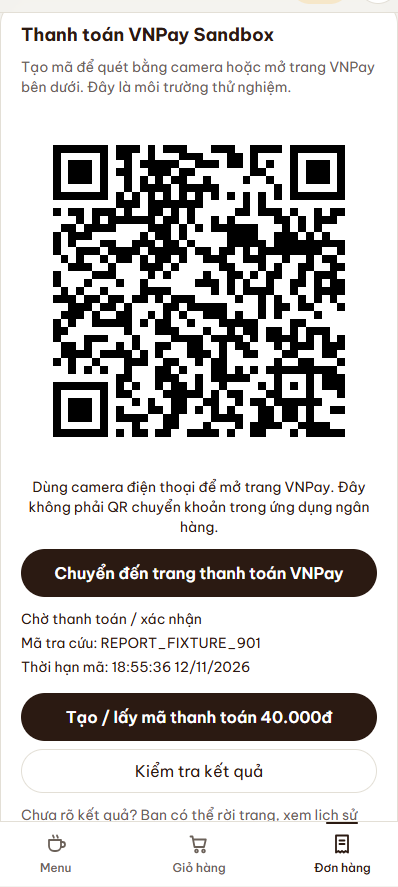
\includegraphics[width=.32\linewidth,height=.40\textheight,keepaspectratio]{assets/vnpay/payment-ui-fixture.png}
\caption{Màn hình QR và nút mở trang VNPay; ảnh UI dùng API fixture với tham chiếu thử}
\end{figure}


\subsection{Kiểm chứng đổi món và thu chênh lệch}
\begin{table}[htbp]\centering\small
\begin{tabularx}{\linewidth}{|p{.13\linewidth}|X|}\hline
\textbf{Ca} & \textbf{Điều kiện cần chứng minh}\\\hline
EX-01 & Đổi bằng giá chuyển credit, hoàn/giữ snapshot đúng, không tạo Payment giả.\\\hline
EX-02 & Đổi cao hơn chỉ thu delta qua VNPay, điểm chỉ tăng theo tiền mới.\\\hline
EX-03 & Món thấp hơn giá trị đã trả bị yêu cầu chọn lại; thiếu kho mới rollback toàn bộ.\\\hline
EX-04 & Đơn PREPARING không được đổi; khách không gọi API quyết định của quầy.\\\hline
EX-05 & Duyệt đổi và bắt đầu pha đồng thời không cùng thành công theo trạng thái cũ.\\\hline
EX-06 & Giá đổi trước gửi làm fingerprint cũ bị từ chối; giá đổi sau gửi không thay báo giá đã lưu.\\\hline
EX-07 & REQUESTED chặn pha; rút yêu cầu đúng version cho phép tiếp tục đơn cũ, version cũ bị chặn.\\\hline
EX-08 & Hàng đợi lọc/phân trang và quyền BARISTA được kiểm ở backend.\\\hline
\end{tabularx}\caption{Các ca kiểm chứng đổi món trong bộ payment-exchange}
\end{table}

Các kịch bản có tại \path{test/payment-exchange.e2e-spec.ts}, thuộc bộ hồi quy đã nêu ở mục~\ref{sec:inventory-tests}; không suy ra một kết quả chạy mới chỉ từ việc bổ sung tài liệu. Kiểm thử giao diện của bản vá 08 sử dụng fixture để kiểm chọn món/giỏ đổi, gửi yêu cầu và thao tác quầy. Ảnh dưới minh họa UI với dữ liệu thử, không phải bằng chứng thu tiền thật.

\begin{figure}[htbp]\centering
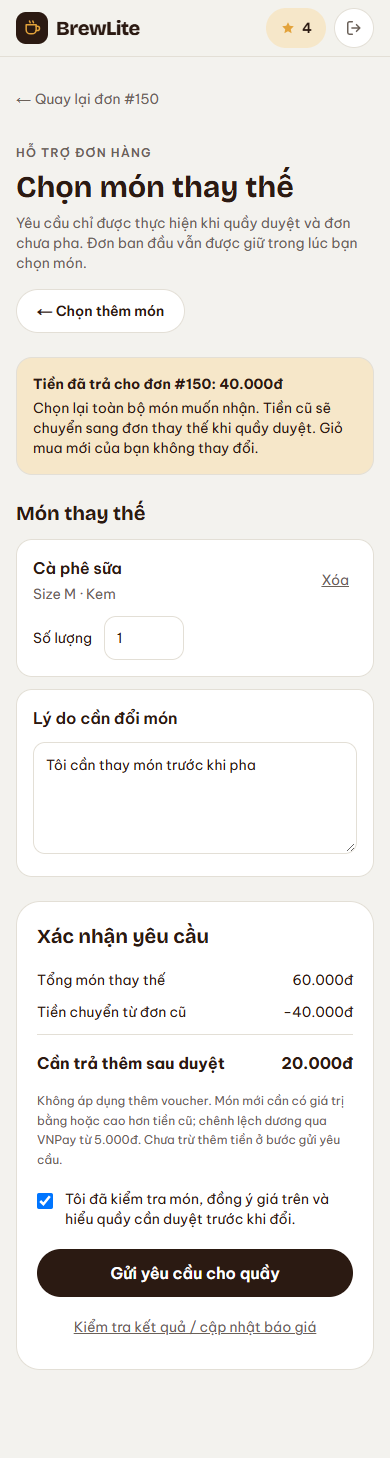
\includegraphics[width=.28\linewidth,height=.38\textheight,keepaspectratio]{assets/exchange/customer-cart-mobile.png}\hfill
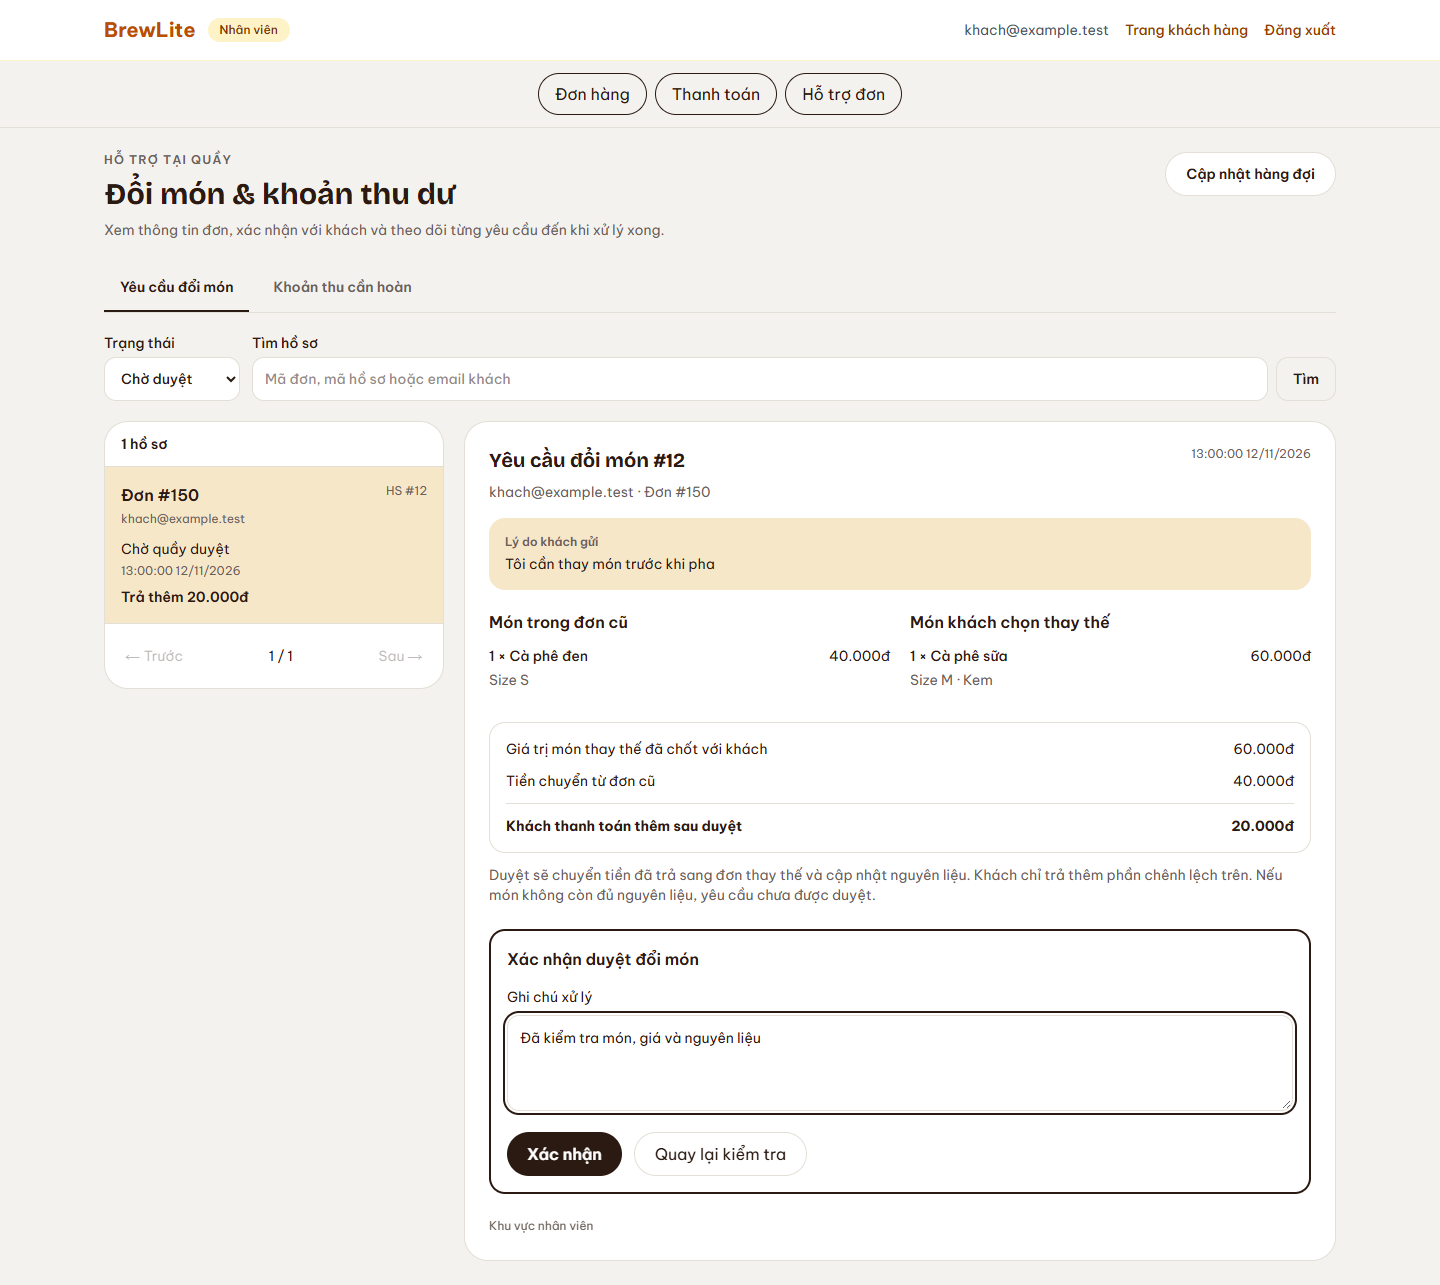
\includegraphics[width=.67\linewidth,height=.38\textheight,keepaspectratio]{assets/exchange/staff-exchange-desktop.png}
\caption{Giỏ đổi của khách và màn hình xử lý của barista (ảnh kiểm thử bằng fixture)}
\end{figure}


\subsection{Kiểm chứng xác thực và phân quyền}
\begin{table}[htbp]\centering\small
\begin{minipage}[t]{.69\linewidth}\vspace{0pt}
\begin{tabularx}{\linewidth}{|p{.13\linewidth}|X|}\hline
\textbf{Ca} & \textbf{Tiêu chí kiểm chứng}\\\hline
AUTH-01 & Đăng ký gửi kèm role BARISTA vẫn tạo CUSTOMER, không tự nâng quyền.\\\hline
AUTH-02 & Login và /auth/me trả vai trò đúng, không có passwordHash.\\\hline
AUTH-03 & Cùng token, đổi role trong database làm quyền gọi /staff/orders thay đổi ở request tiếp theo.\\\hline
AUTH-04 & Route staff thiếu token trả 401; CUSTOMER có token bị 403.\\\hline
AUTH-05 & Khách khác không đọc/hủy/check giao dịch của chủ đơn; dữ liệu và kho không bị thay đổi bởi yêu cầu bị chặn.\\\hline
AUTH-06 & Tiêu chí xác thực token: token sai chữ ký hoặc hết hạn không được đi vào nghiệp vụ được bảo vệ.\\\hline
\end{tabularx}
\end{minipage}\hfill
\begin{minipage}[t]{.27\linewidth}\vspace{0pt}
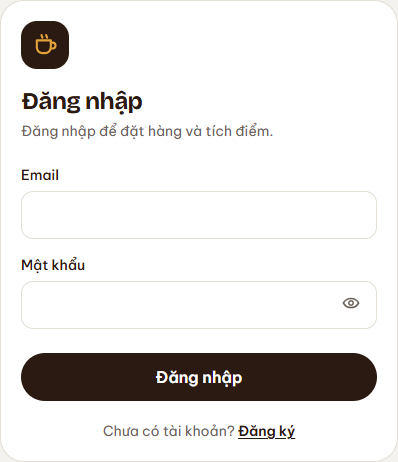
\includegraphics[width=\linewidth]{assets/auth/login-ui.png}
\end{minipage}
\caption{Tiêu chí kiểm chứng quyền và form đăng nhập chụp từ frontend, không có thông tin tài khoản thật}
\end{table}

Ba ca đầu được hiện thực trong \path{test/auth-roles.e2e-spec.ts}. Kiểm tra staff, chủ đơn và giao dịch được phân bố trong các bộ staff-orders, inventory-snapshot và VNPay. AUTH-06 mô tả tiêu chí của cấu hình strategy kiểm chữ ký/hạn; bảng tiêu chí không thay thế log chạy test. Kết quả bộ hồi quy được trình bày theo phạm vi tại mục~\ref{sec:inventory-tests}, không bổ sung số liệu chạy mới ở phần này.



\subsection{Kiểm chứng mã giảm giá và điểm thưởng}
\begin{table}[htbp]\centering\small
\begin{minipage}[t]{.69\linewidth}\vspace{0pt}
\begin{tabularx}{\linewidth}{|p{.18\linewidth}|X|}\hline
\textbf{Ca} & \textbf{Nội dung kiểm tra}\\\hline
KM-01 & Chuẩn hóa hoa/thường, khoảng trắng; mã thiếu/hết hạn/inactive bị từ chối.\\\hline
KM-02 & 120.000đ giảm 10\% còn 108.000đ; làm tròn đúng và không giảm vượt tổng.\\\hline
KM-03 & Mã sai không tạo đơn hoặc trừ nguyên liệu.\\\hline
KM-04 & PAID ghi số dư và một EARN khớp amount sau giảm; dưới ngưỡng không ghi EARN.\\\hline
KM-05 & Request/IPN lặp không nhân đôi điểm; unique chặn EARN trùng.\\\hline
KM-06 & Lỗi cộng điểm rollback settlement; đổi món chỉ cộng điểm trên tiền mới.\\\hline
\end{tabularx}
\end{minipage}\hfill
\begin{minipage}[t]{.27\linewidth}\vspace{0pt}
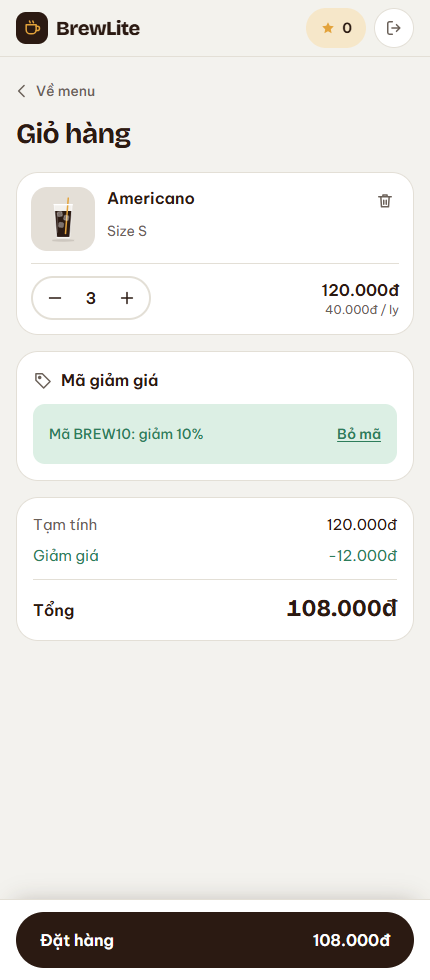
\includegraphics[width=\linewidth]{assets/promotions/voucher-ui-fixture.png}
\end{minipage}
\caption{Tiêu chí kiểm chứng khuyến mãi/điểm và giỏ hàng áp mã với API fixture}
\end{table}

Unit test nằm tại \path{src/promotions/discount.spec.ts}; API test nằm trong promotions, loyalty, staff-orders, VNPay và payment-exchange. Các bộ này kiểm đồng thời kết quả phản hồi, User.loyaltyPoints và dòng sổ EARN. Phạm vi kết quả đã xác minh dùng chung với mục~\ref{sec:inventory-tests}; phần này không bổ sung một số liệu chạy mới. Ảnh giỏ hàng chỉ kiểm chứng hiển thị giảm giá với dữ liệu thử.


\subsection{Kiểm chứng thao tác quầy và realtime}
\begin{table}[htbp]\centering\small
\begin{tabularx}{\linewidth}{|p{.13\linewidth}|X|}\hline
\textbf{Ca} & \textbf{Điều kiện kiểm tra}\\\hline
QUAY-01 & Chỉ BARISTA vào staff API; không hiển thị đơn chưa trả/hủy trong hàng đợi pha.\\\hline
QUAY-02 & Đi đúng PAID--PREPARING--READY--COMPLETED; không tạo thêm Payment, trừ kho hoặc cộng điểm.\\\hline
QUAY-03 & Bỏ bước, lùi bước, bấm lặp và trạng thái/đầu vào sai bị từ chối.\\\hline
QUAY-04 & Hai nhân viên cùng duyệt một đơn: một response 200, một 409, trạng thái cuối nhất quán.\\\hline
QUAY-05 & Hai client WebSocket nhận sự kiện không payload sau commit, đọc API thấy trạng thái mới.\\\hline
QUAY-06 & Rollback và replay không phát thông báo thành công mới; hủy chỉ báo sau khi kho đã hoàn.\\\hline
QUAY-07 & Kết nối lại đọc được trạng thái mới; quyền đọc đơn cá nhân không bị mở rộng.\\\hline
QUAY-08 & Hàng đợi hơn 20 đơn vẫn giữ toàn bộ PAID/PREPARING/READY; nhóm hoàn tất giới hạn riêng.\\\hline
\end{tabularx}\caption{Các ca API và WebSocket cho quy trình quầy}
\end{table}

Các ca có tại \path{test/staff-orders.e2e-spec.ts}; bộ này có client Socket.IO kết nối thật tới ứng dụng test và đọc PostgreSQL để kiểm thứ tự commit/notify. Đây không chỉ là giả lập gọi một hàm emit. Các số liệu bộ hồi quy tham chiếu mục~\ref{sec:inventory-tests}; ảnh dưới sử dụng API fixture để minh họa bảng quầy, không tạo một kết quả chạy backend mới.

\begin{figure}[htbp]\centering
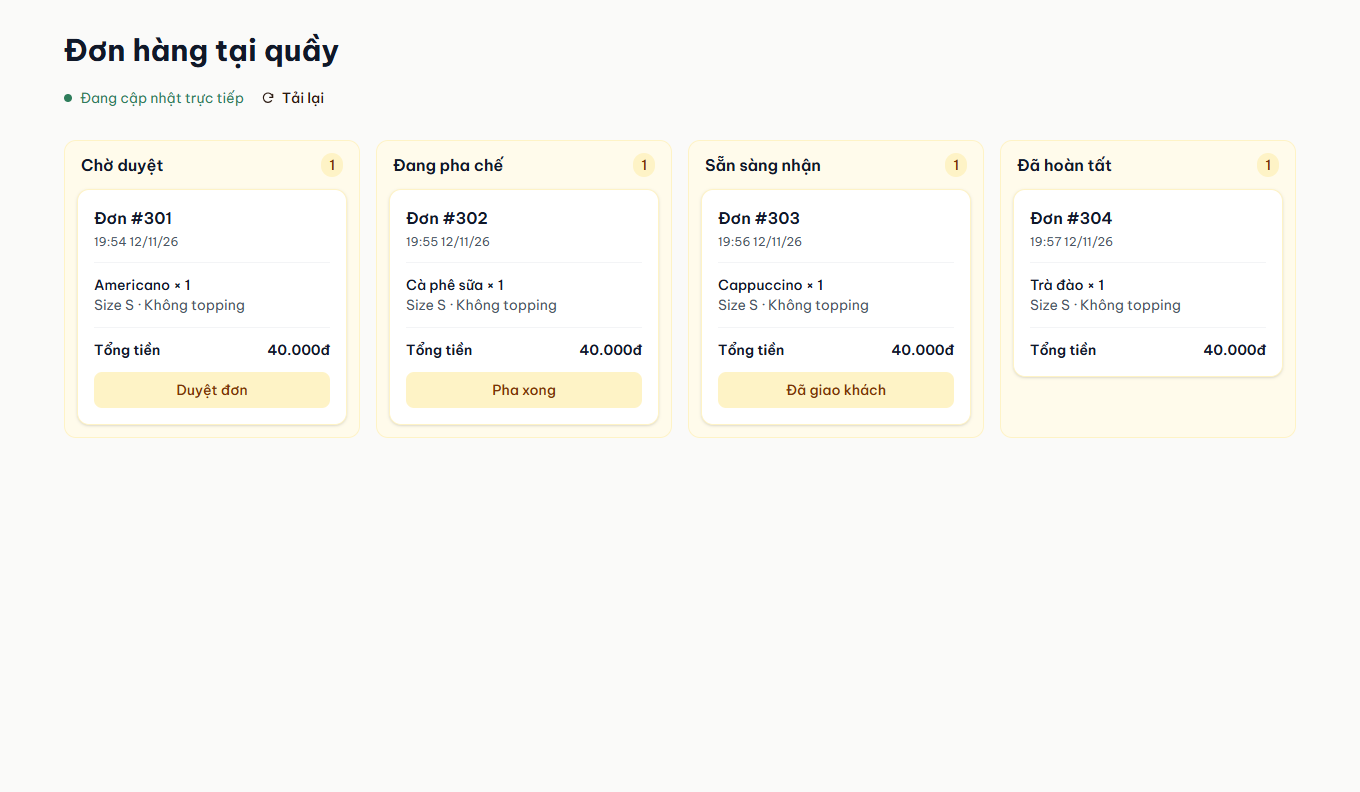
\includegraphics[width=.92\linewidth,height=.27\textheight,keepaspectratio]{assets/staff/board-ui-fixture.png}
\caption{Bốn cột xử lý đơn tại quầy với dữ liệu thử}
\end{figure}


\subsection{Tiêu chí kiểm chứng menu, tùy chọn và giỏ hàng}
\begin{table}[htbp]\centering\small
\begin{tabularx}{\linewidth}{|p{.13\linewidth}|X|}\hline
\textbf{Ca} & \textbf{Điều kiện kiểm chứng}\\\hline
GIO-01 & Menu tải dữ liệu, có trạng thái chờ/rỗng/lỗi; ảnh trống hoặc lỗi có minh họa dự phòng.\\\hline
GIO-02 & Chọn size/topping cập nhật giá; lựa chọn thiếu nguyên liệu không được thêm theo UI, backend kiểm lại khi đặt.\\\hline
GIO-03 & Cùng món/size/topping gộp qty dù thứ tự topping khác; khác tùy chọn tách dòng.\\\hline
GIO-04 & Đổi qty/xóa cập nhật tổng và badge; tải lại vẫn có giỏ, không gây lệch HTML trước hydration.\\\hline
GIO-05 & Chưa đăng nhập đi qua login; gửi order không tin giá client và chỉ xóa giỏ khi đã nhận kết quả tạo đơn.\\\hline
GIO-06 & Mất phản hồi dùng lại checkout key; kiểm tra idempotency chứng minh không tạo thêm Order hoặc giữ thêm kho.\\\hline
\end{tabularx}\caption{Tiêu chí chấp nhận luồng khách chọn món và đặt hàng}
\end{table}

Các ca frontend kiểm ở trình duyệt; phần backend tính lại giá, kiểm input và idempotency có test API trong inventory/order-idempotency. Bảng là tiêu chí kiểm chứng, không thay thế log của một lần chạy browser E2E. Ảnh giao diện trong mục~\ref{sec:catalog-ui} minh họa các màn hình; việc chụp không gửi tạo Order hoặc thanh toán.


\subsection{Kiểm thử chức năng thủ công}
\begin{table}[h!]
\centering
\footnotesize
\begin{tabularx}{\textwidth}{|l|X|X|}
\hline
\textbf{Mã} & \textbf{Thao tác} & \textbf{Kết quả mong đợi} \\ \hline
TC01 & Mở trang chủ & Hiện lưới 4 món có giá; tắt backend thì hiện dòng báo lỗi \\ \hline
TC02 & Mở chi tiết Cappuccino, chọn size L và Trân châu & Thành tiền 60.000đ \\ \hline
TC03 & Thêm cùng món cùng size hai lần & Số lượng tăng thành 2, không thêm dòng mới; tải lại trang giỏ vẫn còn \\ \hline
TC04 & Đăng ký trùng email & Báo lỗi ``Email đã được đăng ký'' \\ \hline
TC05 & Đăng nhập sai mật khẩu & Báo lỗi chung ``Email hoặc mật khẩu không đúng'' \\ \hline
TC06 & Bấm ``Đặt hàng'' ở giỏ hàng & Tạo đơn PENDING, giỏ hàng về trống, tồn kho giảm \\ \hline
TC07 & Thanh toán đơn PENDING bằng Ví & Đơn chuyển PAID, hiện ``Đã nhận thanh toán, chờ quầy xác nhận'' \\ \hline
TC08 & Thanh toán với tùy chọn giả lập lỗi & Đơn chuyển PAYMENT\_FAILED, vẫn thanh toán lại hoặc hủy được \\ \hline
TC09 & Hủy đơn PENDING & Đơn chuyển CANCELLED, tồn kho được hoàn lại \\ \hline
TC10 & Đơn đã PAID & Không có nút hủy; gọi API hủy trả lỗi 409 \\ \hline
TC11 & Nhập mã BREW10 với giỏ 120.000đ & Giảm 12.000đ, tổng 108.000đ; thanh toán xong được 10 điểm \\ \hline
TC12 & Nhập mã không tồn tại & Báo lỗi ``Mã giảm giá không tồn tại'' \\ \hline
\end{tabularx}
\caption{Các ca kiểm thử chức năng thủ công}
\end{table}



\newpage
%%%%%%%%%%%%%%%%%%%%%%%%%%%%%%%%%
\section{Hướng dẫn triển khai}
\subsection{Chạy bằng Docker}
Ở thư mục gốc của dự án (cần mở Docker Desktop):
\begin{lstlisting}[style=brew,language={}]
docker compose up -d db
\end{lstlisting}
Lệnh trên hiện chỉ chạy PostgreSQL ở cổng 5432; backend và frontend phải chạy ở hai terminal riêng. Kiểm tra cổng và DATABASE\_URL nếu máy có nhiều PostgreSQL. Dừng bằng \texttt{docker compose down}; không dùng tùy chọn xóa volume khi cần giữ dữ liệu.

\subsection{Chạy chế độ phát triển}
Terminal backend, từ thư mục gốc:
\begin{lstlisting}[style=brew,language={}]
cd backend
npm.cmd install
npx.cmd prisma generate
npx.cmd prisma migrate status
npm.cmd run start:dev
\end{lstlisting}
Sao lưu trước khi áp dụng thay đổi cấu trúc; dùng \texttt{npx.cmd prisma migrate deploy} cho các migration tăng dần và \texttt{npx.cmd prisma generate} để đồng bộ client. Với database mẫu mới, chủ động chạy \texttt{npx.cmd prisma db seed}. Quá trình triển khai bảo toàn dữ liệu và không reset database vận hành.

Terminal frontend, mở mới tại thư mục gốc:
\begin{lstlisting}[style=brew,language={}]
cd frontend
npm.cmd install
npm.cmd run dev
\end{lstlisting}
Địa chỉ phát triển: web \url{http://localhost:3000}, API mặc định \url{http://localhost:3001}; PORT và cấu hình thực tế có thể thay đổi. Ngrok cho callback Sandbox phải trỏ tới backend, Return URL và IPN URL phải đúng route được khai báo.

\subsection{Biến môi trường}
\begin{table}[h!]
\centering
\footnotesize
\begin{tabularx}{\textwidth}{|p{0.22\linewidth}|p{0.28\linewidth}|X|}
\hline
\textbf{Biến} & \textbf{Nơi dùng} & \textbf{Ý nghĩa} \\ \hline
\texttt{DATABASE\_URL} & backend & Chuỗi kết nối PostgreSQL \\ \hline
\texttt{JWT\_SECRET} & backend & Khóa ký token đăng nhập \\ \hline
\texttt{NEXT\_PUBLIC\_API\_URL} & frontend & Địa chỉ backend mà trình duyệt gọi \\ \hline
\texttt{PORT}, \texttt{FRONTEND\_URL} & backend & Cổng API và địa chỉ frontend để chuyển hướng sau thanh toán \\ \hline
\texttt{VNPAY\_*} & backend & Mã merchant, khóa ký, URL Sandbox, Return/IPN theo cấu hình; không đưa khóa thật vào báo cáo \\ \hline
\end{tabularx}
\caption{Các biến môi trường}
\end{table}

\subsection{Dữ liệu mẫu}
Hệ thống có sẵn 4 sản phẩm (Cà phê sữa 35.000đ, Americano 40.000đ, Cappuccino 45.000đ, Trà đào 39.000đ, tồn kho theo Ingredient và định lượng Recipe, không phải 50 phần cố định cho mỗi món) và mã giảm giá BREW10 giảm 10\%. Tài khoản được tạo ở trang đăng ký.

\section{Đánh giá và hướng phát triển}
\subsection{Giá trị của thiết kế}
Việc tách công thức, định lượng lựa chọn và snapshot giúp hệ thống đồng thời phục vụ bán hàng và bảo toàn tài nguyên lịch sử. Transaction cùng khóa dòng bảo vệ phần nguyên liệu cuối; idempotency bảo vệ request gửi lại; version kiểm soát cập nhật hồ sơ nghiệp vụ. Deadline bền vững phối hợp giữ món với thanh toán và cung cấp thông báo rõ cho khách.
\subsection{Định hướng mở rộng}
Các hướng mở rộng gồm cấu hình định lượng theo từng sản phẩm/size, công cụ nhập và kiểm kê nguyên liệu, phân tích nhu cầu tiêu thụ, quan sát tác vụ nền và tối ưu trải nghiệm đặt lại. Nghiệp vụ giao hàng được xem xét trong phạm vi vận hành cửa hàng, còn báo cáo tập trung vào đặt và nhận món tại quầy.

\section{Kết luận}
BrewLite đã có các luồng chọn món, đặt đơn, thanh toán giả lập/VNPay Sandbox, nghiệp vụ quầy và đổi món. Báo cáo trình bày yêu cầu sản phẩm, thiết kế, hiện thực, kiểm thử và hướng dẫn triển khai để phục vụ bàn giao và bảo trì. Các quy tắc được liên kết với mô hình dữ liệu, hàm hiện thực và kịch bản kiểm thử, giúp giải thích từ nhu cầu nghiệp vụ tới quyết định kỹ thuật.





%%%%%%%%%%%%%%%%%%%%%%%%%%%%%%%%%
\clearpage
\clearpage
\begin{thebibliography}{80}

\bibitem{VNPAYPAY}
VNPAY, \textit{Kết nối cổng thanh toán và API QueryDr},
\url{https://sandbox.vnpayment.vn/apis/docs/thanh-toan-pay/pay.html},
truy cập ngày 12/11/2026.

\bibitem{VNPAYFAQ}
VNPAY, \textit{Câu hỏi thường gặp về tham số và Return/IPN},
\url{https://sandbox.vnpayment.vn/apis/docs/faqs/},
truy cập ngày 12/11/2026.

\bibitem{NEST}
NestJS Documentation,
``\textbf{link: https://docs.nestjs.com}'',
\textit{NestJS - A progressive Node.js framework}, lần truy cập cuối: 11/2026.

\bibitem{NEXT}
Next.js Documentation,
``\textbf{link: https://nextjs.org/docs}'',
\textit{Next.js by Vercel}, lần truy cập cuối: 11/2026.

\bibitem{PRISMA}
Prisma Documentation,
``\textbf{link: https://www.prisma.io/docs}'',
\textit{Prisma ORM}, lần truy cập cuối: 11/2026.

\bibitem{VITEST}
Vitest Documentation,
``\textbf{link: https://vitest.dev}'',
\textit{Vitest - Next generation testing framework}, lần truy cập cuối: 11/2026.

\bibitem{DOCKER}
Docker Documentation,
``\textbf{link: https://docs.docker.com}'',
\textit{Docker and Docker Compose}, lần truy cập cuối: 11/2026.

\bibitem{SCRUM}
Ken Schwaber và Jeff Sutherland,
``\textbf{link: https://scrumguides.org}'',
\textit{The Scrum Guide}, lần truy cập cuối: 11/2026.

\end{thebibliography}
\end{document}
